\documentclass[11pt]{article}
\usepackage{XCharter}
% \usepackage[T1]{fontenc}
\usepackage[utf8]{inputenc}

\usepackage{graphicx, geometry, wrapfig, float, multicol, mathtools, array, csquotes, lscape, setspace}
\usepackage{wrapfig}
\usepackage{multirow}
% \usepackage[compactitem, compactenum]{paralist}
\usepackage{subcaption}
\usepackage[sorting=none]{biblatex}
\addbibresource{bibliography.bib}
\setcounter{biburllcpenalty}{9000}
\usepackage[none]{hyphenat}
\usepackage[dvipsnames]{xcolor}
\usepackage[most]{tcolorbox}
\usepackage{hyperref}
\usepackage{pifont}% http://ctan.org/pkg/pifont
\usepackage{xstring}
\usepackage{txfonts}
\usepackage[none]{hyphenat}
\usepackage{svg}
\usepackage{multicol}
\usepackage{subcaption}  % For subfigures
\usepackage{tikz}
% \usepackage{pgfplots}


\setlength{\parindent}{0pt}

\usepackage{fancyhdr}
\pagestyle{fancy}

\fancyhead{}
\fancyhead[L]{Computer Vision \& Deep Learning}
%\fancyhead[R]{\nouppercase{\rightmark}}
\fancyfoot{}
\fancyfoot[C]{\thepage}
\hypersetup{
    colorlinks=true,
    allcolors=.,
    pdftitle={Computer Vision Report},
    linkcolor=black
}
\geometry{
    top=3.5cm,
    bottom=3.0cm,
    outer=2.5cm,
    inner=2.5cm,
    heightrounded,% <--- added, use it
    % showframe,% <--- just for debugging
    verbose,% <--- just for debugging
}


%%%%% MAIN
\begin{document}

\begin{titlepage}
    \begin{center}
        \vspace*{1cm}
        \huge
        \textbf{Medical image segmentation using advanced deep techniques}\\
        \vspace{0.5cm}
        \Large
        \textbf{Comparison between UNet and Mae+Unetr}
        \vspace{0.5cm}
        
            
        \vspace{0.5cm}
        \large
        Project report\\
        Computer Vision \& Deep Learning Course
            
        \vspace{3.5cm}
        \begin{minipage}{0.4\textwidth}
        \begin{flushleft} \large
        \emph{Authors:}\\
        \vspace{5mm}
        Bonanni Lorenzo\\ \textit{VR495629} \\
        \vspace{5mm}
        Filippi Virginia\\ \textit{VR495315}
        \end{flushleft}
        \end{minipage}
        ~
        \begin{minipage}{0.4\textwidth}
        \begin{flushright} \large
        \emph{Professors:}\\
        \vspace{5mm}
        Vittorio Murino
        \end{flushright}
        \end{minipage}\\[2cm]
            
        \vfill
        \vspace{0.8cm}
            
        \large
        Master degree in Artificial Intelligence\\
        Department of Computer Science\\
        University of Verona\\
            
    \end{center}
\end{titlepage}


\newpage
\tableofcontents

\newpage
\section{Introduction}
\subsection{Motivation and rationale}
Image segmentation is a crucial topic in image processing and computer vision with applications in various fields such as scene understanding, medical image analysis, robotic perception, video surveillance, augmented reality, and image compression.

In particular, segmentation of medical images is a critical task in the analysis of medical images. This process, which consists of dividing an image into regions that correspond to different anatomical structures or areas of interest, is fundamental for many clinical applications, including diagnosis, disease monitoring and treatment planning.

In recent years, deep learning has demonstrated remarkable capabilities in extracting valuable insights from medical images \cite{GhaffarNia2023EvaluationOA}.
Deep learning models, trained on large datasets, can recognise complex patterns and features that may not be readily discernible to the human eye \cite{hosny_artificial_2018, kumar_artificial_2023}.
These algorithms can even provide a new perspective about what image features should be valued to support decisions \cite{waldstein2020unbiased}. One of the key advantages of AI in medical imaging is its ability to enhance the accuracy and efficiency of disease diagnosis \cite{GhaffarNia2023EvaluationOA, plested2022deep}. Through this process, AI can assist healthcare professionals in detecting abnormalities, identifying specific structures, and predicting disease outcomes \cite{plested2022deep, alowais_revolutionizing_2023}. By leveraging machine learning algorithms, AI systems can analyze medical images with speed and precision, aiding in identifying early-stage diseases that may be difficult to detect through traditional methods. This early detection is crucial as it can lead to timely interventions, potentially saving lives and improving treatment outcomes \cite{GhaffarNia2023EvaluationOA, hosny_artificial_2018, kumar_artificial_2023}. Furthermore, AI has opened up new possibilities in image segmentation and quantification. By employing sophisticated algorithms, AI can accurately delineate structures of interest within medical images, such as tumors, blood vessels, or cells \cite{bioengineering9090467, bioengineering9090475, 9066969}. This segmentation capability is invaluable in treatment planning, as it enables clinicians to precisely target areas for intervention, optimize surgical procedures, and deliver targeted therapies \cite{VANDESANDE2021111}.\\

In this report, we perform critical evaluation and comparison of two distinct methodologies for medical image segmentation: UNet\cite{ronneberger2015u} and a hybrid approach combining Masked Autoencoders (MAE)\cite{He_2022_CVPR} and UNETR\cite{hatamizadeh2022unetr}.
The selection of UNet and the MAE-UNETR hybrid stems from their prominence and efficacy in the field of medical image analysis. UNet, a convolutional neural network architecture, has demonstrated robust performance in semantic segmentation tasks, particularly in medical imaging, due to its ability to capture both local and global features effectively. Conversely, the MAE-UNETR hybrid integrates the strengths of masked autoencoders for feature extraction with the transformer-based UNETR model, offering a potentially enhanced segmentation capability by leveraging attention mechanisms and hierarchical representations.


%%%%%%%%%%%%%%%%%%%%%%%%%%%%%%%%%%%%%%%%%%%%%%%%%%%%%%%%%%%%%%%%%%
\subsection{State of the Art}
% TODO add something
% Describe the state of the art relevant to the project
% What results or techniques do you plan to exploit? What are the weak points of the SoA methods, and which ones need to be improved? Why? How?

Image segmentation is an operation fundamental in artificial vision. It consists of dividing one image into several parts or regions that belong to the same class. This process of grouping is based on specific criteria, for example, colour or texture.

\subsubsection*{Types of Image Segmentation} 
There are three main types of image segmentation: semantic segmentation, instance segmentation and panoptic segmentation, each one addressing different aspects of scene understanding. 
\begin{itemize}
    \item \textbf{Semantic segmentation}: it involves classifying each pixel in an image into a specific category or class, without distinguishing between different instances of the same class. 
    \item \textbf{Instance segmentation}: it's like semantic segmentation, but it also distinguishes between different instances of the same class, providing a unique label for each individual object in the image.
    \item \textbf{Panoptic segmentation}: it's a combination of both semantic and instance segmentation. It aims to provide a comprehensive understanding of the visual scene by assigning a category label to each pixel and a unique instance ID to each individual object, regardless of the class.
\end{itemize}

\subsubsection*{Traditional methods vs Deep Learning}

Traditional methods, which rely on classic image processing techniques like thresholding and edge detection, have long been the foundation for segmenting medical images. These methods are straightforward and efficient, but they often struggle with the complexity and variability of medical images. On the other hand, deep learning techniques, especially convolutional neural networks (CNNs), have revolutionized medical image segmentation. Deep learning models can automatically learn patterns and features from data, improving segmentation accuracy and adaptability across different types of medical images. While deep learning methods require more computational resources and may be prone to overfitting, they offer flexibility and scalability that traditional methods cannot match.

Neural nets that perform the task of segmentation typically are based on CNNs or use an encoder-decoder structure. The encoder extracts features of an image through narrower and deeper filters. If the encoder is pre-trained on a task like an image or face recognition, it then uses that knowledge to extract features for segmentation (transfer learning). The decoder then over a series of layers inflates the encoder’s output into a segmentation mask resembling the pixel resolution of the input image.

Many deep learning models are quite adept at performing the segmentation task. Some of these are:
\begin{itemize}
    \item \textbf{UNet} \cite{ronneberger2015u}: it is one of the most used state-of-the-art techniques, based on fully convolutional neural networks. It was primarily proposed for medical purposes, i.e., to detect tumors in the lungs and brain. The architecture is explained in section 3.1. It has been extensively studied and many variations of it are used, including Attention UNet \cite{oktay2018attention}, UNet++ \cite{zhou2018unet++}, Dense UNet \cite{cai2020dense}.
    \item \textbf{SegNet} \cite{badrinarayanan2017segnet}: it's also a deep fully convolutional network designed especially for semantic pixel-wise segmentation. Like U-Net, SegNet’s architecture also consists of encoder and decoder blocks. The SegNet differs from other neural networks in the way it uses its decoder for upsampling the features. The decoder network uses the pooling indices computed in the max-pooling layer which in turn makes the encoder perform non-linear upsampling. This eliminates the need for learning to upsample. SegNet is primarily designed for scene-understanding applications.

    \begin{figure}[h]
        \centering
        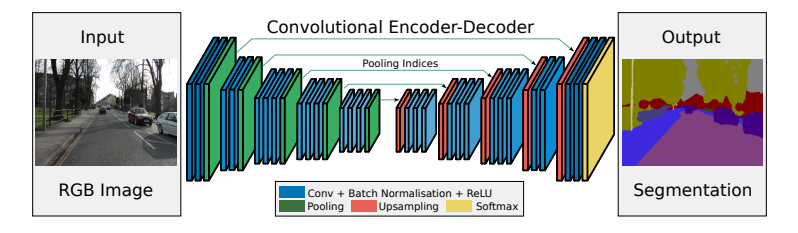
\includegraphics[scale=0.75]{images/segnet.png}
        \caption{SegNet architecture}
        \label{fig:segnet}
    \end{figure}
    
    \item \textbf{DeepLab} \cite{chen2018encoder}: it's primarily a convolutional neural network (CNN) architecture. Unlike the other two networks, it uses features from every convolutional block and then concatenates them to their deconvolutional block. The neural network uses the features from the last convolutional block and upsamples it like the fully convolutional network (FCN). It uses the atrous convolution or dilated convolution method for upsampling. The advantage of atrous convolution is that the computation cost is reduced while capturing more information.
\end{itemize}

Foundation models have also been used for image segmentation, which divides an image into distinct regions or segments. Unlike language models, which are typically based on transformer architectures, foundation models for image segmentation often use convolutional neural networks (CNNs) designed to handle image data.
\begin{itemize}
    \item \textbf{Segment Anything Model (SAM)} \cite{kirillov2023segment}: is considered the first foundation model for image segmentation. 
    SAM is built on the largest segmentation dataset to date, with over 1 billion segmentation masks. 
    It is trained to return a valid segmentation mask for any prompt, where a prompt can be foreground or background points, a rough box or mask, freeform text, or general information indicating what to segment in an image.
    Under the hood, an image encoder produces a one-time embedding for the image, while a lightweight encoder converts any prompt into an embedding vector in real time. 
    These two information sources are combined in a lightweight decoder that predicts segmentation tasks.
\end{itemize}

\begin{figure}[h]
    \centering
    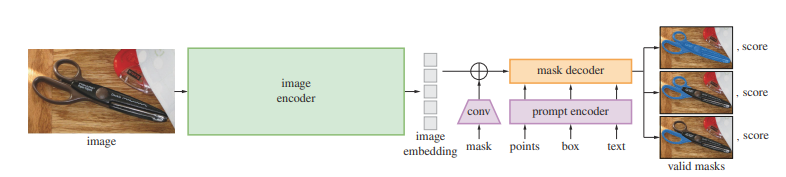
\includegraphics{images/sam.png}
    \caption{Segment Anything Model (SAM) overview.}
    \label{fig:sam}
\end{figure}


\subsubsection*{Limitations of deep learning methods} 
As image segmentation continues to advance, future directions will focus on improving segmentation accuracy, integrating deep learning with traditional techniques, and exploring new applications in various fields. \\Auto-segmentation with the Segment Anything Model (SAM) is a promising direction that can reduce manual intervention and improve accuracy. \\Integration of deep learning with traditional techniques can also help to overcome the limitations of individual techniques and improve overall performance. With ongoing research and development, we can expect image segmentation to continue to make significant contributions to various fields and industries.\\

Of course, deep learning methods have significantly advanced the field of medical image segmentation, but they also have some limitations:
\begin{itemize}
    \item \textbf{Data requirements}: deep methods typically require large amounts of labelled data for training. In the medical field, obtaining such data can be challenging due to privacy issues, the effort required to label medical images, and the need for expert knowledge to provide accurate labels.
    \item \textbf{Computational resources}: training deep learning models can be computationally intensive, requiring powerful hardware and potentially long training times.
    \item \textbf{Generalizability}: while deep learning models can achieve high performance on the data they were trained on, they may not generalize well to new data or different tasks.
    \item \textbf{Segmentation accuracy}: despite the great achievements of medical image segmentation in recent years, medical image segmentation based on deep learning has still encountered difficulties in research. For example, the segmentation accuracy is not high, the number of medical images in the dataset is small and the resolution is low.
    \item \textbf{Clinical requirements}: the inaccurate segmentation results are unable to meet the actual clinical requirements.
\end{itemize}



%%%%%%%%%%%%%%%%%%%%%%%%%%%%%%%%%%%%%%%%%%%%%%%%%%%%%%%%%%%%%%%%%%%%%%%%%%
\section{Objectives}
The primary objective of this project is to evaluate and compare two distinct methodologies for medical image segmentation: UNet and a novel hybrid approach combining Masked Autoencoders (MAE) with UNETR. By conducting a comprehensive analysis, we aim to understand their relative strengths, weaknesses, and performance across different datasets.
Our evaluation will be based on two key metrics:
\begin{enumerate}
    \item \textbf{Training Time}: We measure the time required for each algorithm to train on the respective datasets.
    \item \textbf{Test Dice Metric}: The Dice coefficient (also known as the Sørensen–Dice coefficient) quantifies the overlap between the predicted segmentation mask and the ground truth. It provides insight into the segmentation accuracy.
\end{enumerate}
By analyzing these metrics, we aim to determine which algorithm performs better in terms of both computational efficiency (training time) and segmentation quality (Dice metric). These findings will guide practitioners in selecting the most suitable approach for specific medical image segmentation tasks.

\section{Methodology}

\subsection{UNet}

The \textbf{U-Net} architecture \cite{ronneberger2015u} is a widely used deep learning architecture for semantic segmentation, particularly in the field of biomedical image segmentation. It follows an encoder-decoder cascade structure, where the encoder gradually compresses information into a lower-dimensional representation, and the decoder decodes this information back to the original image dimension. The two paths are more or less symmetric, and so the architecture gets an overall U-shape, which leads to the name U-Net.

The main properties of this architecture are:
\begin{itemize}
    \item U-Net learns segmentation in an \textbf{end-to-end} setting.
    \item It requires very few annotated images (approx. 30 images for application in general) using augmented training data with deformations to use the available annotated samples more efficiently. This leads also to efficient training considering only a smaller amount of data while maintaining speed and accuracy, making UNet useful in the medical field where annotated data can be limited.
\end{itemize}

\begin{figure}[H]
    \centering
    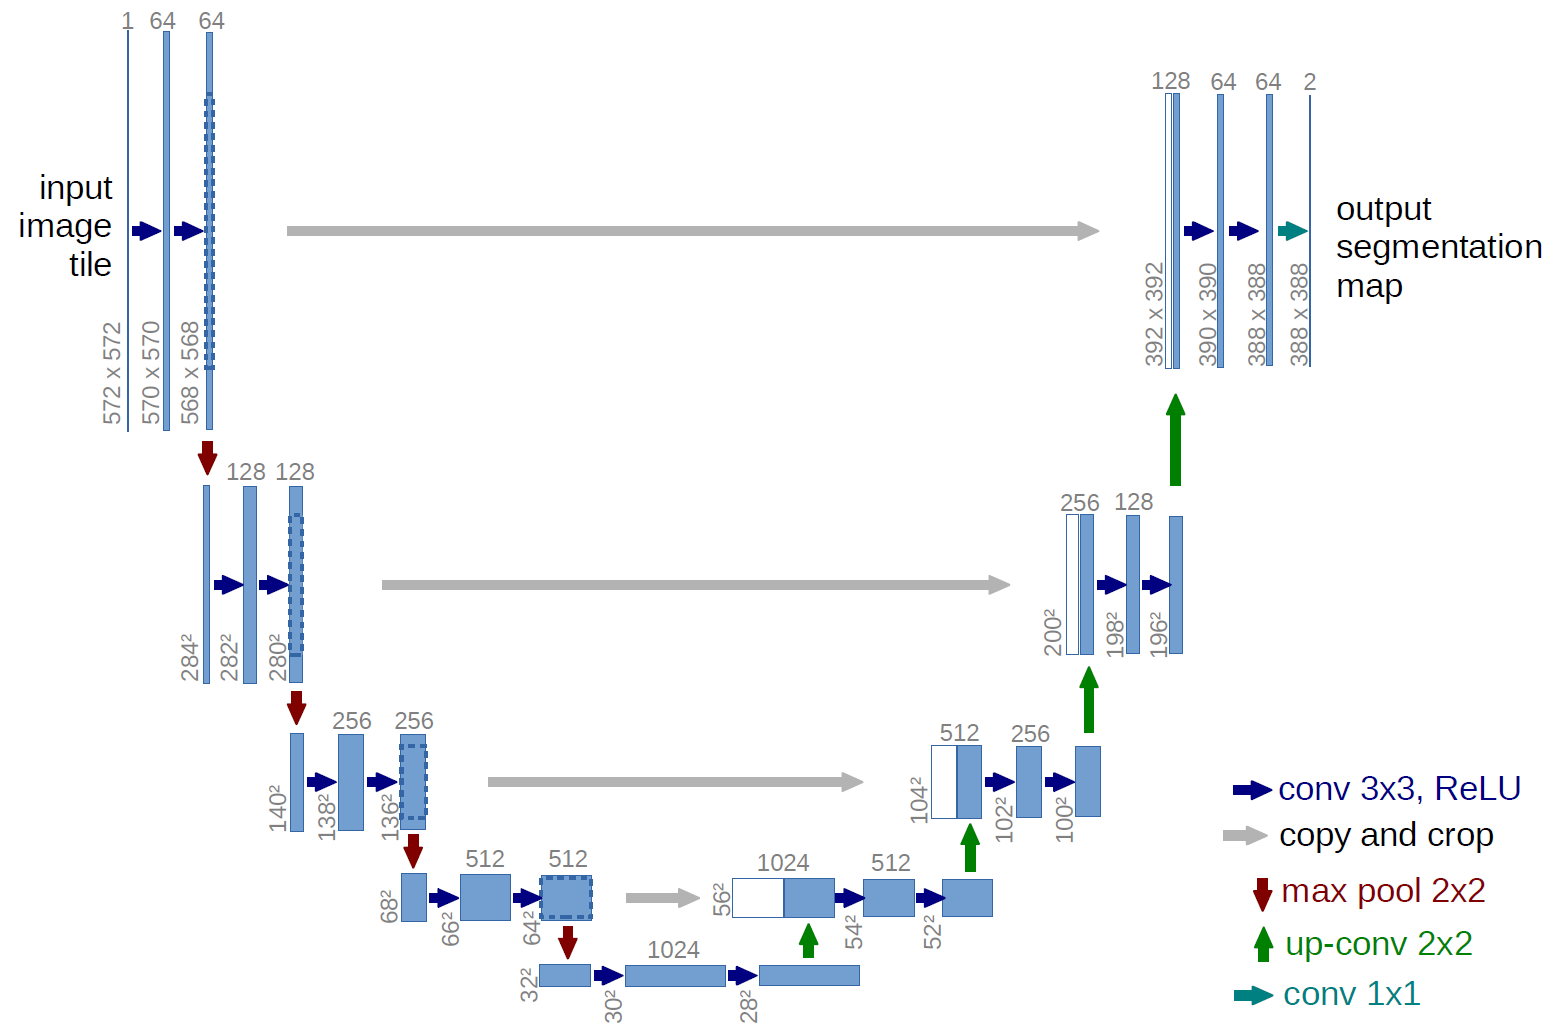
\includegraphics[scale=0.25]{images/u-net-architecture.png}
    \caption{U-net architecture (example for 32x32 pixels in the lowest resolution). Each blue box corresponds to a multi-channel feature map. The number of channels is denoted on top of the box. The x-y-size is provided at the lower left edge of the box. White boxes represent copied feature maps. The arrows denote the different operations.}
    \label{fig:u-net-architecture}
\end{figure}

The first part of the architecture - the \textbf{contractive path} - captures the global context of the image and reduces the sizes, identifying the relevant features in the input image. It consists of the repeated application of convolutions 3x3, each followed by a max 2x2 pooling operation for downsampling.\\

The second part of the architecture - the \textbf{expansive path} - creates a high-resolution segmentation map of the original image and enables precise localization (combining high-resolution features from the contracting path and the upsampled output of this phase). Each step consists of an upsampling of the feature map followed by a 2x2 convolution ("up-convolution", a concatenation with the corresponding cropped feature map from the contracting path, and two 3x3 convolutions, to increase the resolution. The upsampling part has a large number of feature channels, allowing the network to propagate context information to higher-resolution layers. The skip connections help to recover the spatial information lost in the contracting path, helping to locate the features more accurately.\\

At the final layer, a 1x1 convolution is used to map each 64-component feature vector to the desired number of classes. So, each pixel in the output image represents a label that corresponds to a particular object or class in the input image. In this case, the output map is a binary segmentation map where each pixel represents a foreground or background region.\\

This architecture is particularly suitable for semantic segmentation in the medical field because it is effective even with a limited dataset and a higher accuracy.

%%%%%%%%%%%%%%%%%%%%%
\subsection{UNETR}

UNETR\cite{hatamizadeh2022unetr}, or UNEt TRansformer, is a transformer-based architecture for medical image segmentation. This architecture utilizes a pure vision transformer as the encoder to capture the global contextual representations using the U-shape of the UNet architecture \cite{ronneberger2015u} but without relying on CNNs for feature extraction. The CNN-based decoder, connected with the encoder via skip connections, combines the extracted representations at different resolutions and predicts the segmentation output.\\

It was introduced to overcome the problem in FCNN-based approaches, in which the localized receptive fields limit the learning capabilities to relatively small regions without learning long-range dependencies, resulting in sub-optimal segmentations.\\
Transformer models, created mainly for Natural Language Processing tasks, have been applied to various tasks. Compared to FCNN models, they can model and learn long-range information and capture the global context using a sequence of 1D patch embeddings (as the word sequences in NLP).

In this paper, they used a transformer for a 3D medical image segmentation task seeing it as a 1D sequence-to-sequence prediction, learning contextual information from the embedded input patches. Combining the transformer-based encoder and the CNN-based decoder, they can properly capture both global and localized information.

\begin{figure}[H]
    \centering
    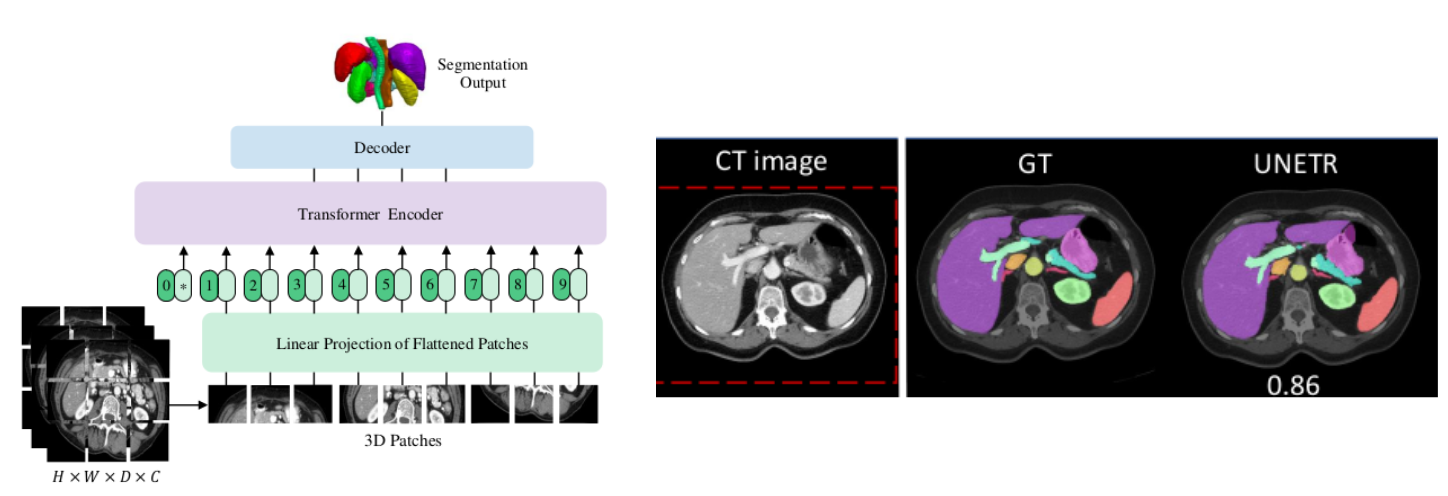
\includegraphics[scale=0.3]{images/unetr_1.png}
    \caption{General architecture of UNETR and an example of possible results from BTCV challenge dataset \cite{landman2015miccai}}
    \label{fig:unetr1-architecture}
\end{figure}

To pass the input to the encoder, the 3D input volume is partitioned into a series of consistent and non-overlapping patches. These patches are then projected into an embedding space through the application of a linear layer. Following this, the sequence is augmented with a positional embedding and serves as the input for the transformer encoder.
The transformer model encodes representations across various layers, and these encoded representations are subsequently extracted and combined with a decoder through skip connections to maintain at the end the same size as the input. This process is essential for predicting the output segmentation.

\begin{figure}[H]
     \centering
     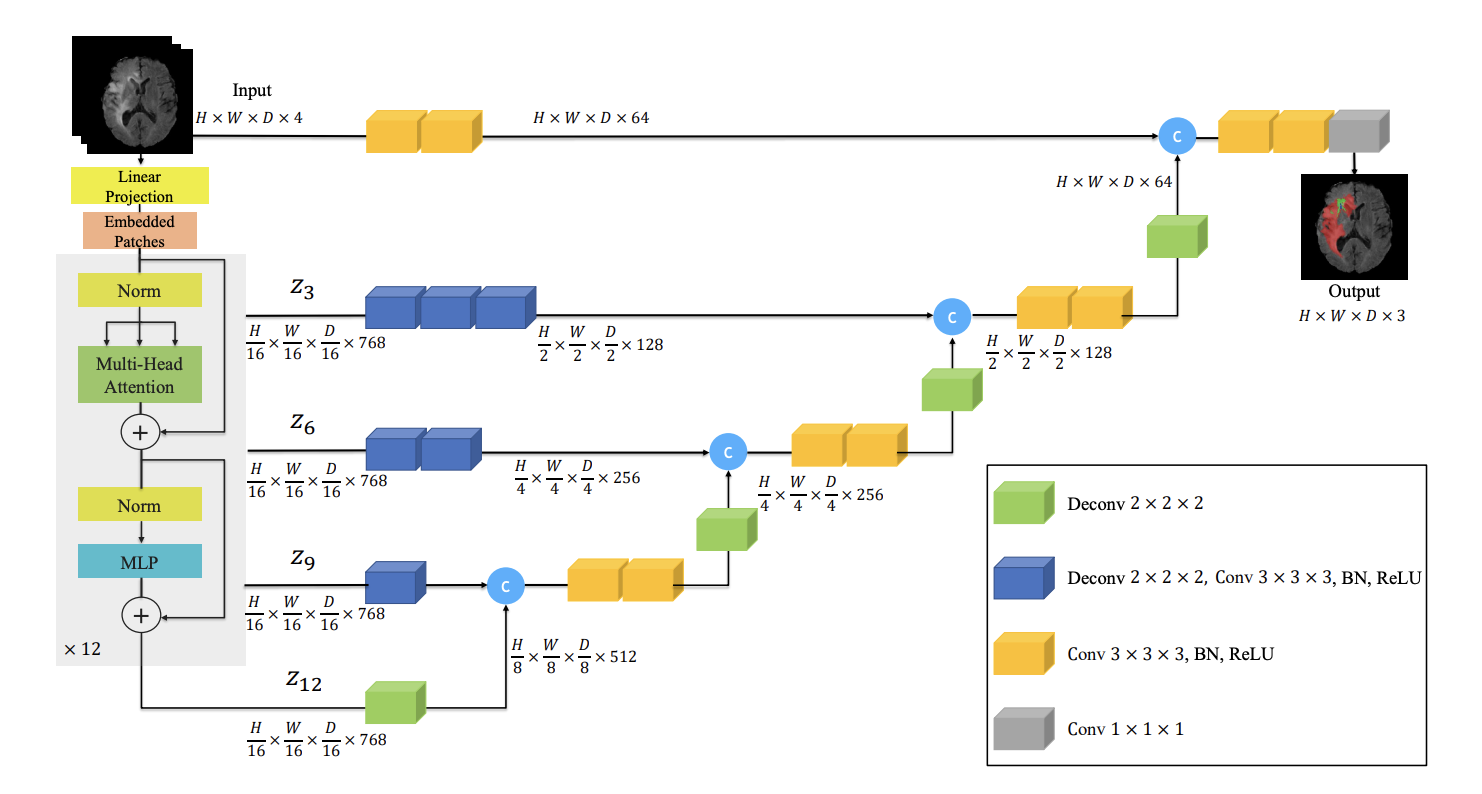
\includegraphics[scale=0.6]{images/unetr2.png}
     \caption{UNETR architecture details}
     \label{fig:unetr2-architecture}
\end{figure}


%%%%%%%%%%%%%%%%%%%%%
\subsection{Masked Autoencoders}

Masked Autoencoders (MAE) \cite{he2022masked}  are a type of autoencoder neural network architecture designed for self-supervised learning and feature representation. Autoencoders, in general, aim to learn meaningful compressed representations of input data. The core idea behind MAEs is the introduction of a masking mechanism to the traditional autoencoder structure to learn more meaningful and lower-dimensional representations and use them to reconstruct missing or masked portions of input images.

\begin{figure}[H]
    \centering
    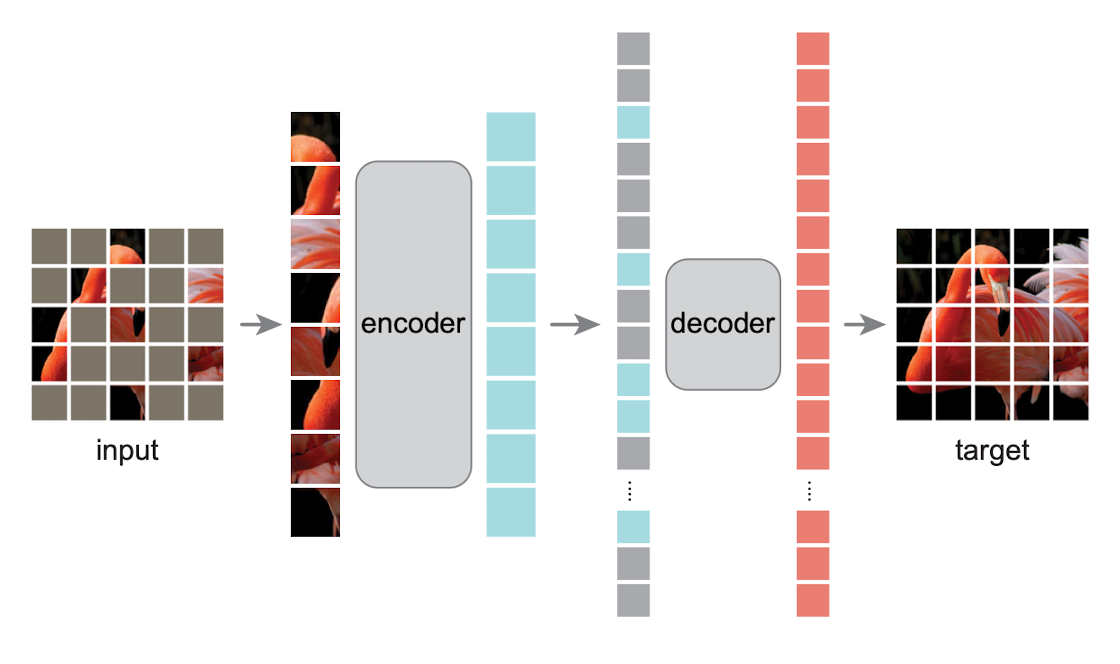
\includegraphics[scale=0.25]{images/mae1.png}
    \caption{MAE Architecture}
    \label{fig:mae1-architecture}
\end{figure}

The architecture consists of an asymmetric encoder-decoder setup. The ViT encoder takes the input data and applies to them a masking mechanism, which selectively ignores or sets certain elements to zero masking portions of the input images.
The encoder processes only the visible subset of patches (without mask tokens), mapping it to a lower-dimensional representation.
The decoder reconstructs the entire image from the latent representations and mask tokens (adding positional embeddings to have location information). The masking information is propagated through the decoding process to ensure that only the relevant information is used in the reconstruction.\\

Training involves minimizing the reconstruction loss, which encourages the encoder to learn useful features, strengthened by the masking mechanism. Regularization terms can be added to encourage sparsity in the latent space, promoting a more compact and meaningful representation.\\
The authors found that masking a high proportion of the input image, e.g., 75\%, yields a nontrivial and meaningful self-supervisory task, allowing also the model to generalize very well training with only a fraction of compute and memory.\\

Moreover, this network exhibits remarkable adaptability to diverse tasks. The MAE decoder is only used during pre-training to perform the image reconstruction task. Then a big advantage in this architecture lies in the flexibility of the decoder architecture, as it can be effortlessly modified independently of the encoder design.

%%%%%%%%%%%%%%%%%%%%%%%%%%%%%%%%%%%%%%%%%%%
\subsection{MAE+UNetr}
Our approach begins with an MAE encoder, which maps the input image into a latent space, capturing intermediary representations along the way. This latent space serves as input to the MAE decoder, which reconstructs the original image. Subsequently, we utilize the original image, the latent space, the intermediary representations, and the reconstructed images as input to a U-NetR decoder. The U-NetR decoder generates a segmentation mask, allowing us to extract meaningful features and enhance the segmentation performance.

\begin{figure}[H]
    \centering
    \includesvg[scale=0.7]{images/arch.svg}
    \caption{MAE+UNETR architecture}
    \label{fig:complete-arch}
\end{figure}

% \begin{figure}[H]
%     \centering
%     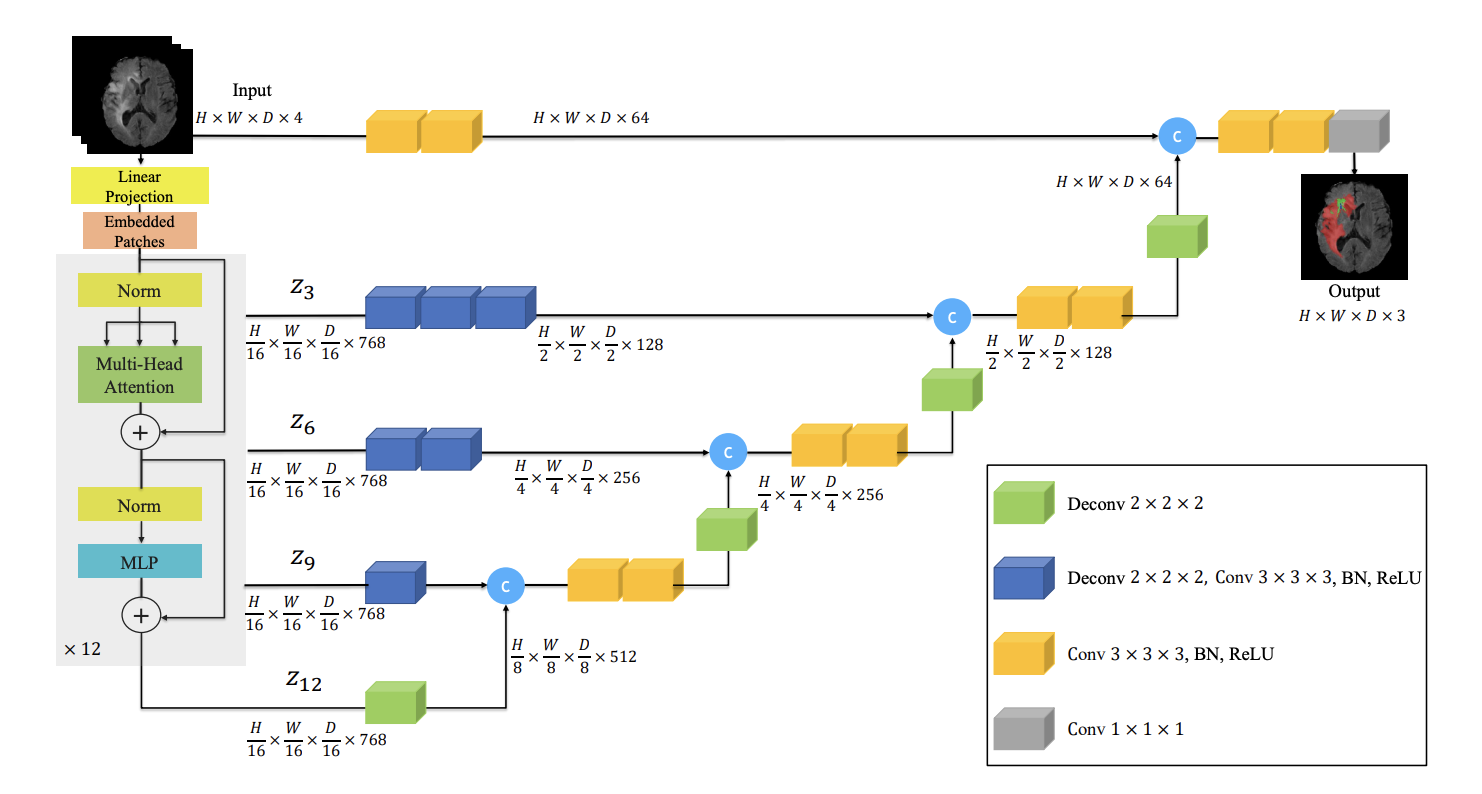
\includegraphics[scale=0.5]{images/unetr2.png}
%     \caption{UNETR architecture - 2}
%     \label{fig:unetr2-architecture}
% \end{figure}
\section{Experiments}
\subsection{Dataset choice}\label{dataset}
Two datasets were used to compare the behaviour of the individual algorithms as data and phases vary and their functioning.
The datasets used are:
\begin{enumerate}
    \item \textbf{Breast Ultrasound Images Dataset} \cite{al2020dataset} \footnote{Link: \texttt{\url{https://www.kaggle.com/datasets/aryashah2k/breast-ultrasound-images-dataset/}}}\\The dataset is composed of medical images of breast cancer using ultrasound scan. This dataset is categorized into 3 classes - normal, benign, malignant - that we have transformed into 2 classes - normal and patients with tumor. The data collected in 2018 include breast ultrasound images women in ages between 25 and 75 years old, with a total of 600 female patients. The dataset consists of 780 images in PNG format. The ground truth images are presented with original images.
    \item \textbf{Brain Tumor Segmentation} \cite{Cheng2017} \footnote{Link: \texttt{\url{https://www.kaggle.com/datasets/nikhilroxtomar/brain-tumor-segmentation}}} \\This brain tumor dataset containing 3064 T1-weighted contrast-inhanced images from 233 patients with three kinds of brain tumor: meningioma (708 slices), glioma (1426 slices), and pituitary tumor (930 slices). 
    \item \textbf{CVC-ClinicDB} \cite{PMID:25863519} \footnote{Link: \texttt{\url{https://www.kaggle.com/datasets/balraj98/cvcclinicdb}}}\\
    CVC-ClinicDB is a database of frames extracted from colonoscopy videos. The dataset is composed by 612 still images from 29 different sequences. Each image has its associated manually annotated ground truth covering the polyp. This dataset was obtained from the official CVC-ClinicDB Challenge's homepage: \url{https://polyp.grand-challenge.org/CVCClinicDB/} 
\end{enumerate}

\begin{figure}[]
    \centering
    \begin{subfigure}{1\textwidth}
        \centering
        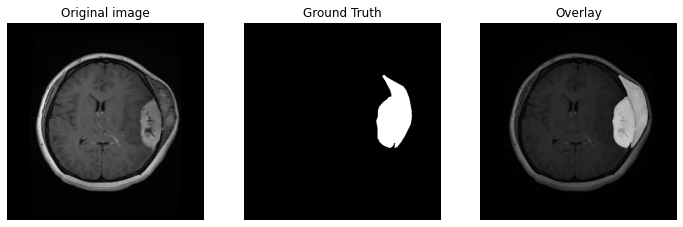
\includegraphics[width=\linewidth]{images/bts1.png}
        \caption{Brain Tumor Segmentation}
        \label{fig:bts1}
    \end{subfigure}

    \vspace{1em}
    
    \begin{subfigure}{1\textwidth}
        \centering
        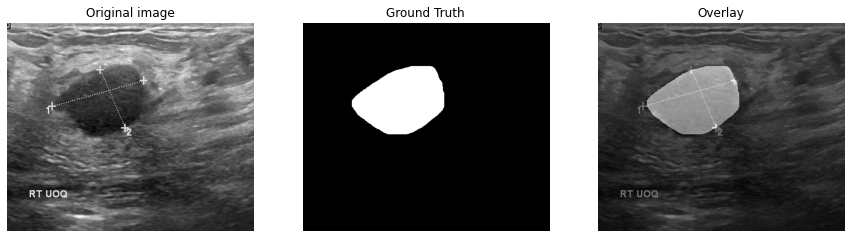
\includegraphics[width=\linewidth]{images/busi1.png}
        \caption{Breast Tumor Segmentation}
        \label{fig:busi1}
    \end{subfigure}

    \vspace{1em}  % Add vertical space between subfigures

    \begin{subfigure}{1\textwidth}
        \centering
        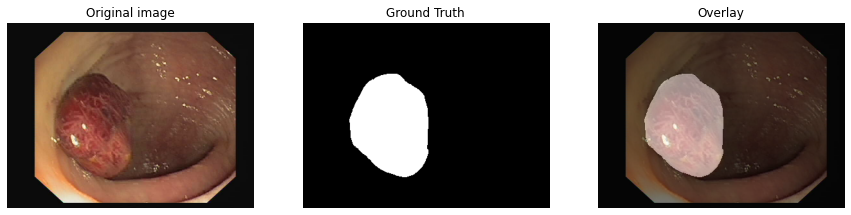
\includegraphics[width=\linewidth]{images/cvc1.png}
        \caption{Polyp Segmentation from Colonoscopy}
        \label{fig:cvc1}
    \end{subfigure}
    \caption{Example Images from the Datasets}
    \label{fig:combined}
\end{figure}


%%%%%%%%%%%%%%%%%%%%%%%%%%%%%%%%%%%%%%%%%%%%%%%%%%%%%%%%%%%%%%%%%%%%%%%%%%
% Preprocessing and parameters of the model/train/test
\subsection{Data Preprocessing}
First, we load all the images from our dataset. If any images is not already in RGB format, we convert it to RGB to ensure consistency in color channels. Next, we employ the HuggingFace VIT Mae image processor %footnote 
for normalization. This step ensures that pixel values are scaled appropriately using the \texttt{ImageNet} mean and standard deviation. After normalization, we resize all images to a uniform size of 224x224 pixels. These resized images are then converted to \texttt{PyTorch} tensors, which are the preferred data format for deep learning models. \\For masks, we follow a simpler process: resizing the mask images to match the desired dimensions (224x224) and converting them to tensors.\\Finally, we split our dataset into three subsets: the \textbf{training set} (70\% of the data), the \textbf{validation set} (15\% for hyperparameter tuning), and the \textbf{test set} (15\% for evaluating model performance on unseen examples).

% \footnote{\textit{\url{https:\/\/huggingface.co\/docs\/transformers\/v4.37.2\/en\/model_doc\/vit#transformers.ViTImageProcessor}}}
\newpage

\subsection{Training}

\subsubsection{Cross-Entropy Loss}
Cross-entropy Loss is a commonly used loss function in deep learning. It quantifies the dissimilarity between the predicted probability distribution and the actual probability distribution (ground truth) of a set of events or classes.

If there are $K$ classes, and $y_i$ represents the true distribution (a one-hot encoded vector with 1 at the true class index and 0 elsewhere), and $\hat{y}_i$ represents the predicted distribution, the cross-entropy loss formula is defined as follows:
$$CE(y, \hat{y}) = - \sum{i=1}{K}{y_i log(\hat{y}_i)}$$

The goal during training is to minimise this loss, so the model is learning to make its predicted probability distribution ($\hat{y}$) as close as possible to the true distribution ($y$).

There are two primary types of cross-entropy loss functions:
\begin{itemize}
    \item \textit{Binary cross-entropy loss}: used with only two possible classes or labels: positive and negative or true and false.
    \item \textit{Categorical cross-entropy loss}: Used in multi-class classification tasks.
\end{itemize}

Cross-entropy loss has several advantages, including its ability to penalize confidently wrong predictions more heavily, making it suitable for training models in classification tasks. Additionally, it provides a smooth and differentiable objective function, which is crucial for gradient-based optimization algorithms used in training neural networks.

\subsubsection{Dice Loss}
The Dice Loss, also known as the Sørensen–Dice coefficient, is a loss function commonly used in image segmentation tasks, suitable for tasks where the class of interest occupies a small portion of the image, like in medical image segmentation.
The Dice Loss is derived from the Dice coefficient, which is a similarity measure between two sets. In binary image segmentation, the Dice coefficient is given by:
$$Dice(A, B) = \frac{2 \cdot |A \bigcap B|}{|A| + |B|}$$
where $A$ is the set of pixels in the predicted segmentation mask, and $B$ is the set of pixels in the ground truth mask.
The Dice coefficient ranges from 0 to 1, where 0 indicates no overlap between the predicted and true masks, and 1 indicates a perfect match.

The Dice loss is then defined as the complement of the Dice coefficient to ensure it behaves as a loss function:
$$DiceLoss(A,B) = 1 - Dice(A, B)$$

This loss function is designed to be minimized during the training of a segmentation model. The goal is to encourage the model to produce segmentation masks that have a high overlap with the ground truth.

In the context of deep learning, the Dice loss is often applied to each class independently in multi-class segmentation problems. The overall loss for a model predicting K classes is the sum of the Dice losses for each class.

Dice loss is popular in medical image segmentation tasks where imbalances between foreground and background classes are common. It helps address issues associated with class imbalance by focusing on the relative overlap between predicted and true masks rather than absolute pixel-wise differences.

\subsubsection{DiceCE Loss}
The DiceCE Loss is a hybrid loss that compute both Dice loss and Cross Entropy loss, and return the weighted sum of these two losses.
The DiceCE Loss can be expressed as:
$$DiceCE(A,B) = \alpha \cdot Dice(A,B) + \beta \cdot CrossEntropy(A,B)$$
where $Dice(A,B)$ is the Dice loss, $CrossEntropy(A,B)$ is the Cross-Entropy loss, and $\alpha, \beta$ are the weighting parameters that control the influence of each loss term.

The Dice loss component encourages accurate pixel-wise predictions and is effective in handling class imbalance. On the other hand, the Cross-Entropy loss penalizes differences in the predicted probability distribution compared to the true distribution.

The choice of $\alpha$ and $\beta$ depends on the segmentation task's specific requirements and the dataset's characteristics.By adjusting these parameters, one can prioritize the correctness of the predicted distribution or the overlap between predicted and true masks.

The DiceCE loss is particularly useful when dealing with imbalanced datasets or when there is a need to strike a balance between capturing fine details in the segmentation masks and ensuring a high level of overall segmentation accuracy. It combines the strengths of both Dice and Cross-Entropy losses to provide a more flexible and adaptive loss function for training segmentation models.

\subsection{Training}
Each network, U-Net and MAE+UNETR, underwent meticulous training procedures tailored to its specific architecture and objectives. Throughout this section, we illuminate the distinctive approaches adopted for training each model, elucidating the rationale behind these methodologies and their implications on model performance.

Despite their architectural disparities, both U-Net and MAE+UNETR converge under the shared umbrella of the \texttt{Adam} optimizer. Furthermore, the hyperparameters guiding the training of these models were selected through a rigorous grid search process.
\subsubsection{Mae+Unetr}
The training strategy for the Mae+UNETR network comprises two distinct phases aimed at optimizing the convergence and alignment of its constituent architectures: the Masked Autoencoder (MAE) and the UNETR.\\

The Masked Autoencoder (MAE) component within the Mae+UNETR architecture is pre-trained leveraging resources provided by Hugging Face. Leveraging pre-trained models from Hugging Face offers numerous advantages, including access to large-scale pre-training data and advanced pre-training strategies, which can significantly enhance the model's representation learning capabilities.\\

By integrating pre-trained MAE components into the Mae+UNETR architecture, we capitalize on the wealth of knowledge and expertise embedded within these pre-trained models, facilitating more efficient convergence and superior performance across diverse datasets.\\

Through the subsequent phases of training, we further refine and fine-tune the UNETR component to align and synergize with the pre-trained MAE, leveraging the combined strengths of both architectures to achieve optimal performance across various evaluation metrics and datasets. This section elucidates the intricacies of the training process and the methodologies employed at each stage.
\begin{enumerate}
    \item \textbf{Warm-Up Phase}: At the onset of training, we initiate a warm-up phase designed to harmonize the operations of the MAE and UNETR components. During this phase, the entire network undergoes training while maintaining a constant learning rate denoted as the $WARM-UP\;LR$. This constant learning rate fosters alignment between the two disparate components by ensuring synchronized learning dynamics. The warm-up phase persists for a predefined number of epochs denoted as $WARM-UP \;EPOCHS$. The batch size utilized during the warm-up phase is set to 16.
    \item \textbf{Fine-Tuning Phase}: Following the completion of the warm-up phase, the training regimen transitions into the fine-tuning phase. In this stage, the UNETR component of the Mae+UNETR network assumes the spotlight, while the MAE component remains frozen, thus preserving its learned features. The fine-tuning process is orchestrated through a sophisticated learning rate scheduler designed to optimize convergence and mitigate overfitting. The learning rate scheduler operates in a step-wise exponential manner, dynamically adjusting the learning rate throughout the training process. The formula for the learning rate scheduler is represented as:
    \begin{equation*}
        scheduler_{lr} * (decay\_factor^{epoch // 20})
    \end{equation*}
    By adhering to this structured training regimen, the Mae+UNETR network undergoes comprehensive optimization, leveraging the warm-up and fine-tuning phases to align its constituent architectures and foster robust convergence. The fine-tuning phase persists for a designated number of epochs denoted as $FINE\_TUNING\;EPOCHS$. The batch size utilized during the fine-tuning phase is set to 64.
\end{enumerate}
Below is a table describing the parameters for each dataset used in the training of the Mae+UNETR network:

\begin{table}[htbp]
\begin{center}
\begin{tabular}{p{2cm}cc}
\textbf{Dataset} & \textbf{Warm-Up Epochs} & \textbf{Fine-Tuning Epochs} \\
CVC  & 100 & 100 \\
BUSI & 50  & 150 \\
BTS  & 50  & 10 \\
\end{tabular}
\caption{Training Parameters for Each Dataset}
% \label{tab:dataset-parameters}
\end{center}
\end{table}

For each dataset, the values of Decay Factor, Scheduler LR, and Warm-Up LR are respectively set to 0.9, 1e-3 and 1e-4.

\begin{figure}[H]
    \centering
    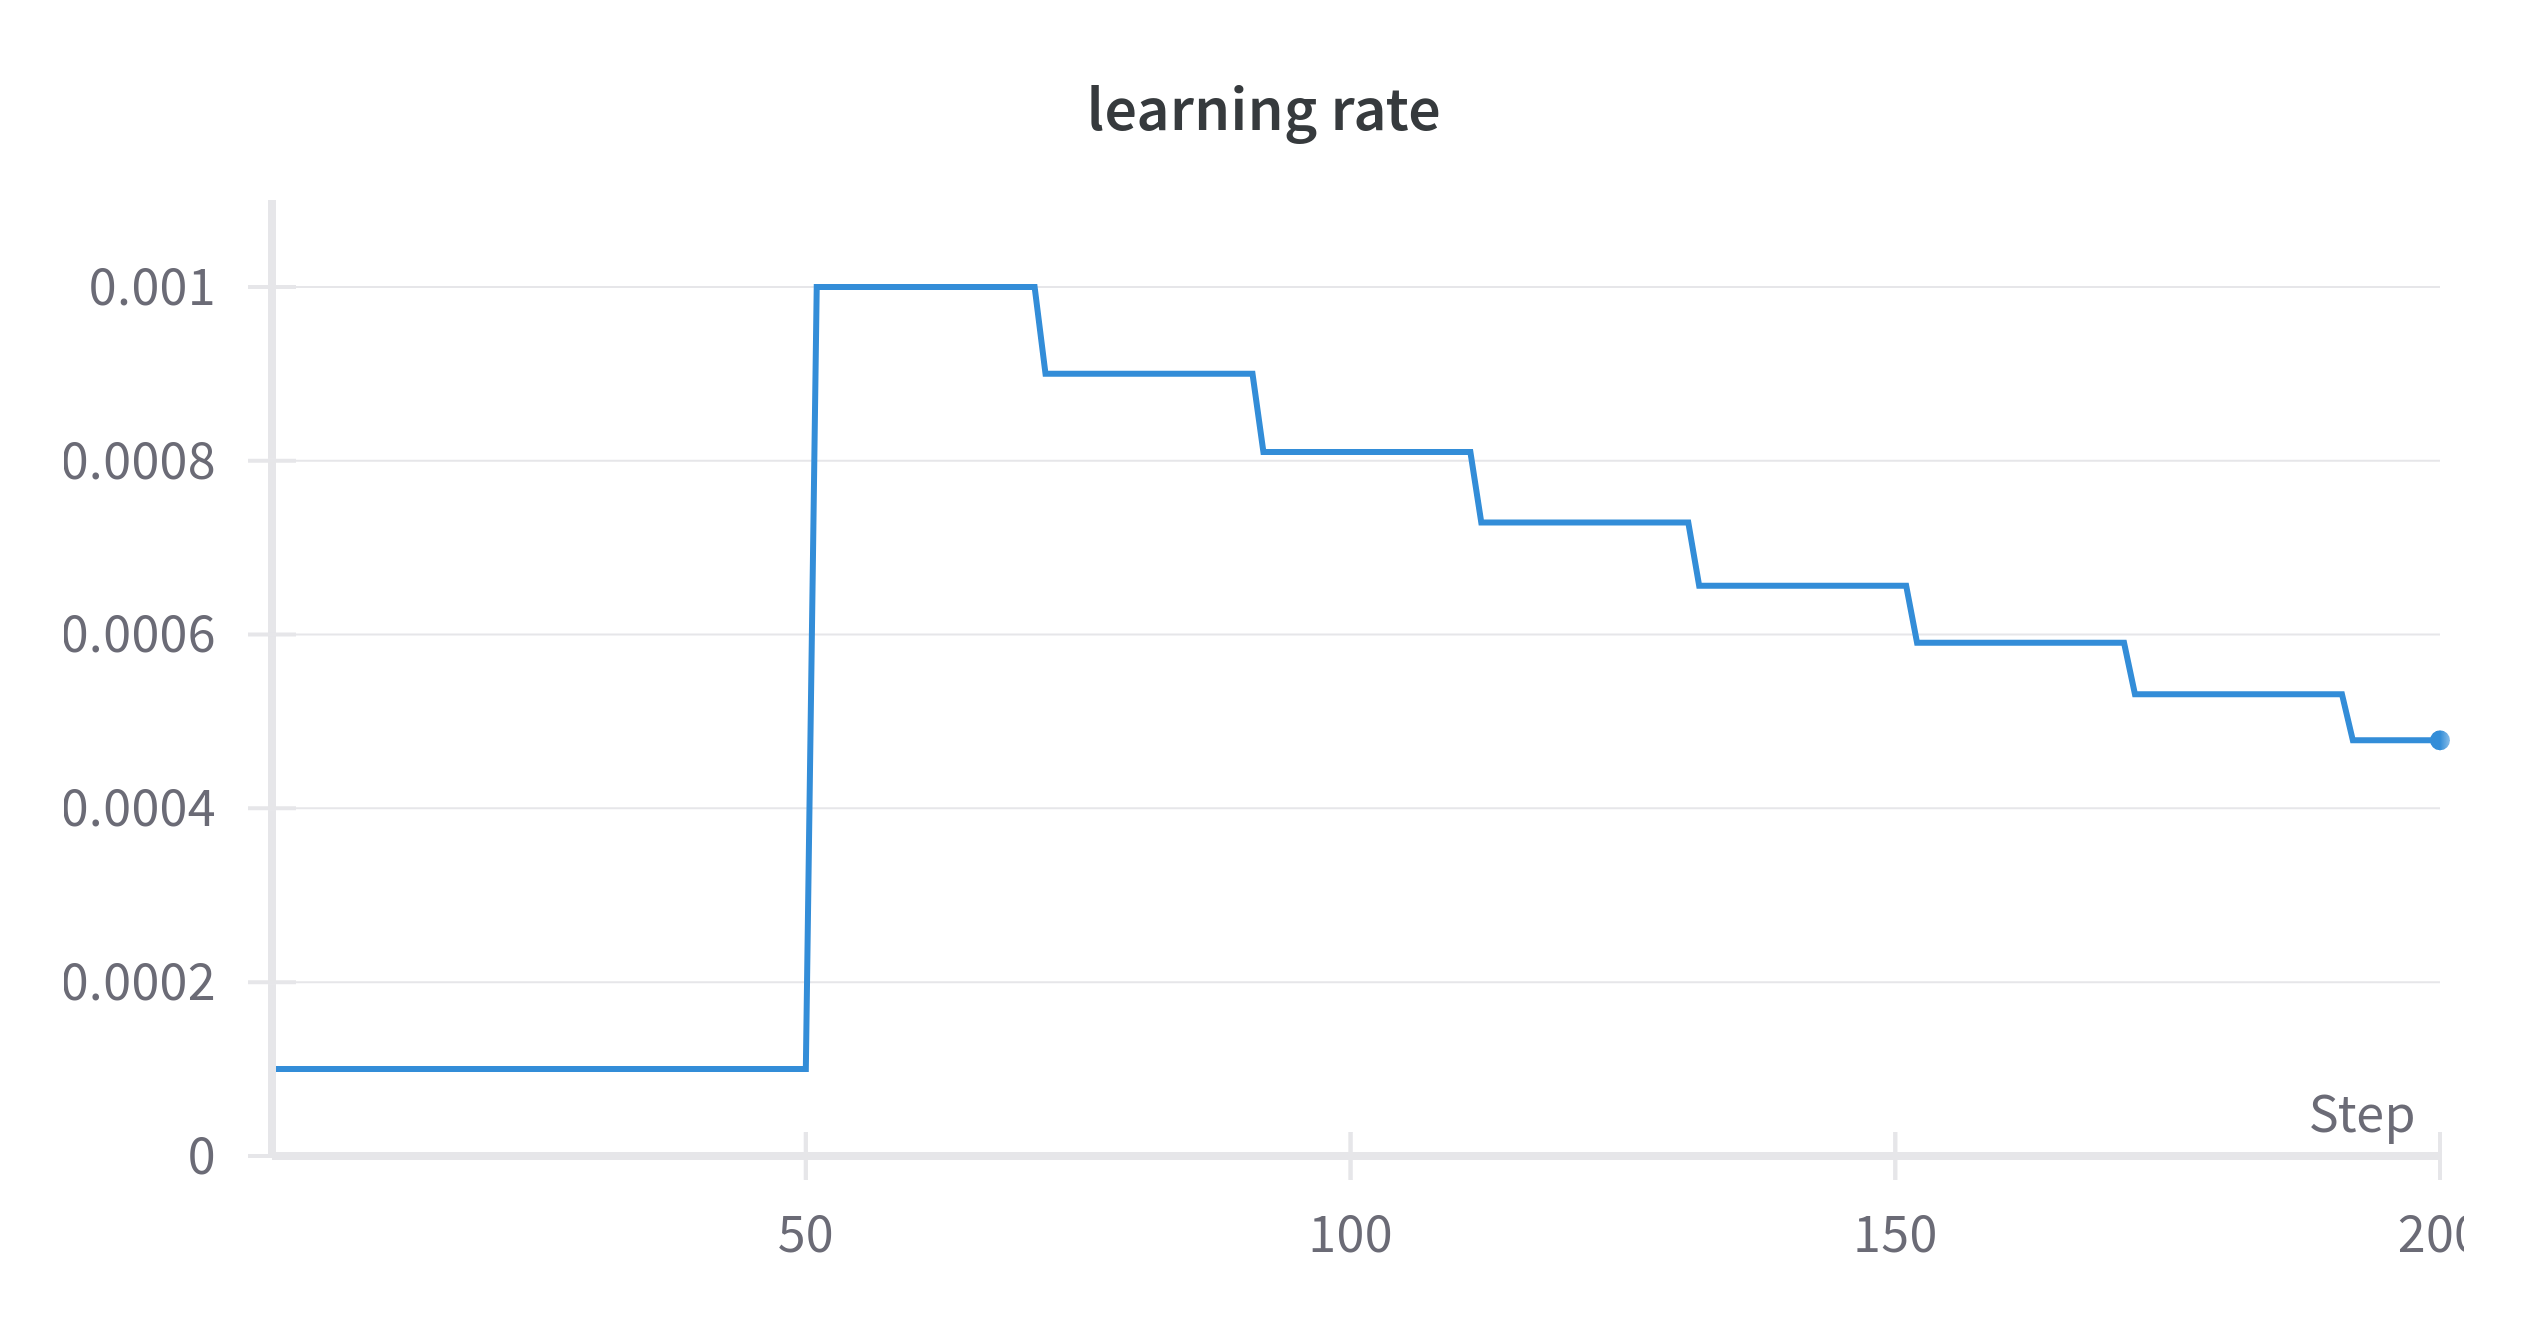
\includegraphics[scale=0.1]{images/lr_decay.png}
    \caption{Example of the change in learning rate during training}
    \label{fig:lr_change}
\end{figure}

\begin{figure}[htbp]
    \centering
    \begin{subfigure}{0.45\textwidth}
        \centering
        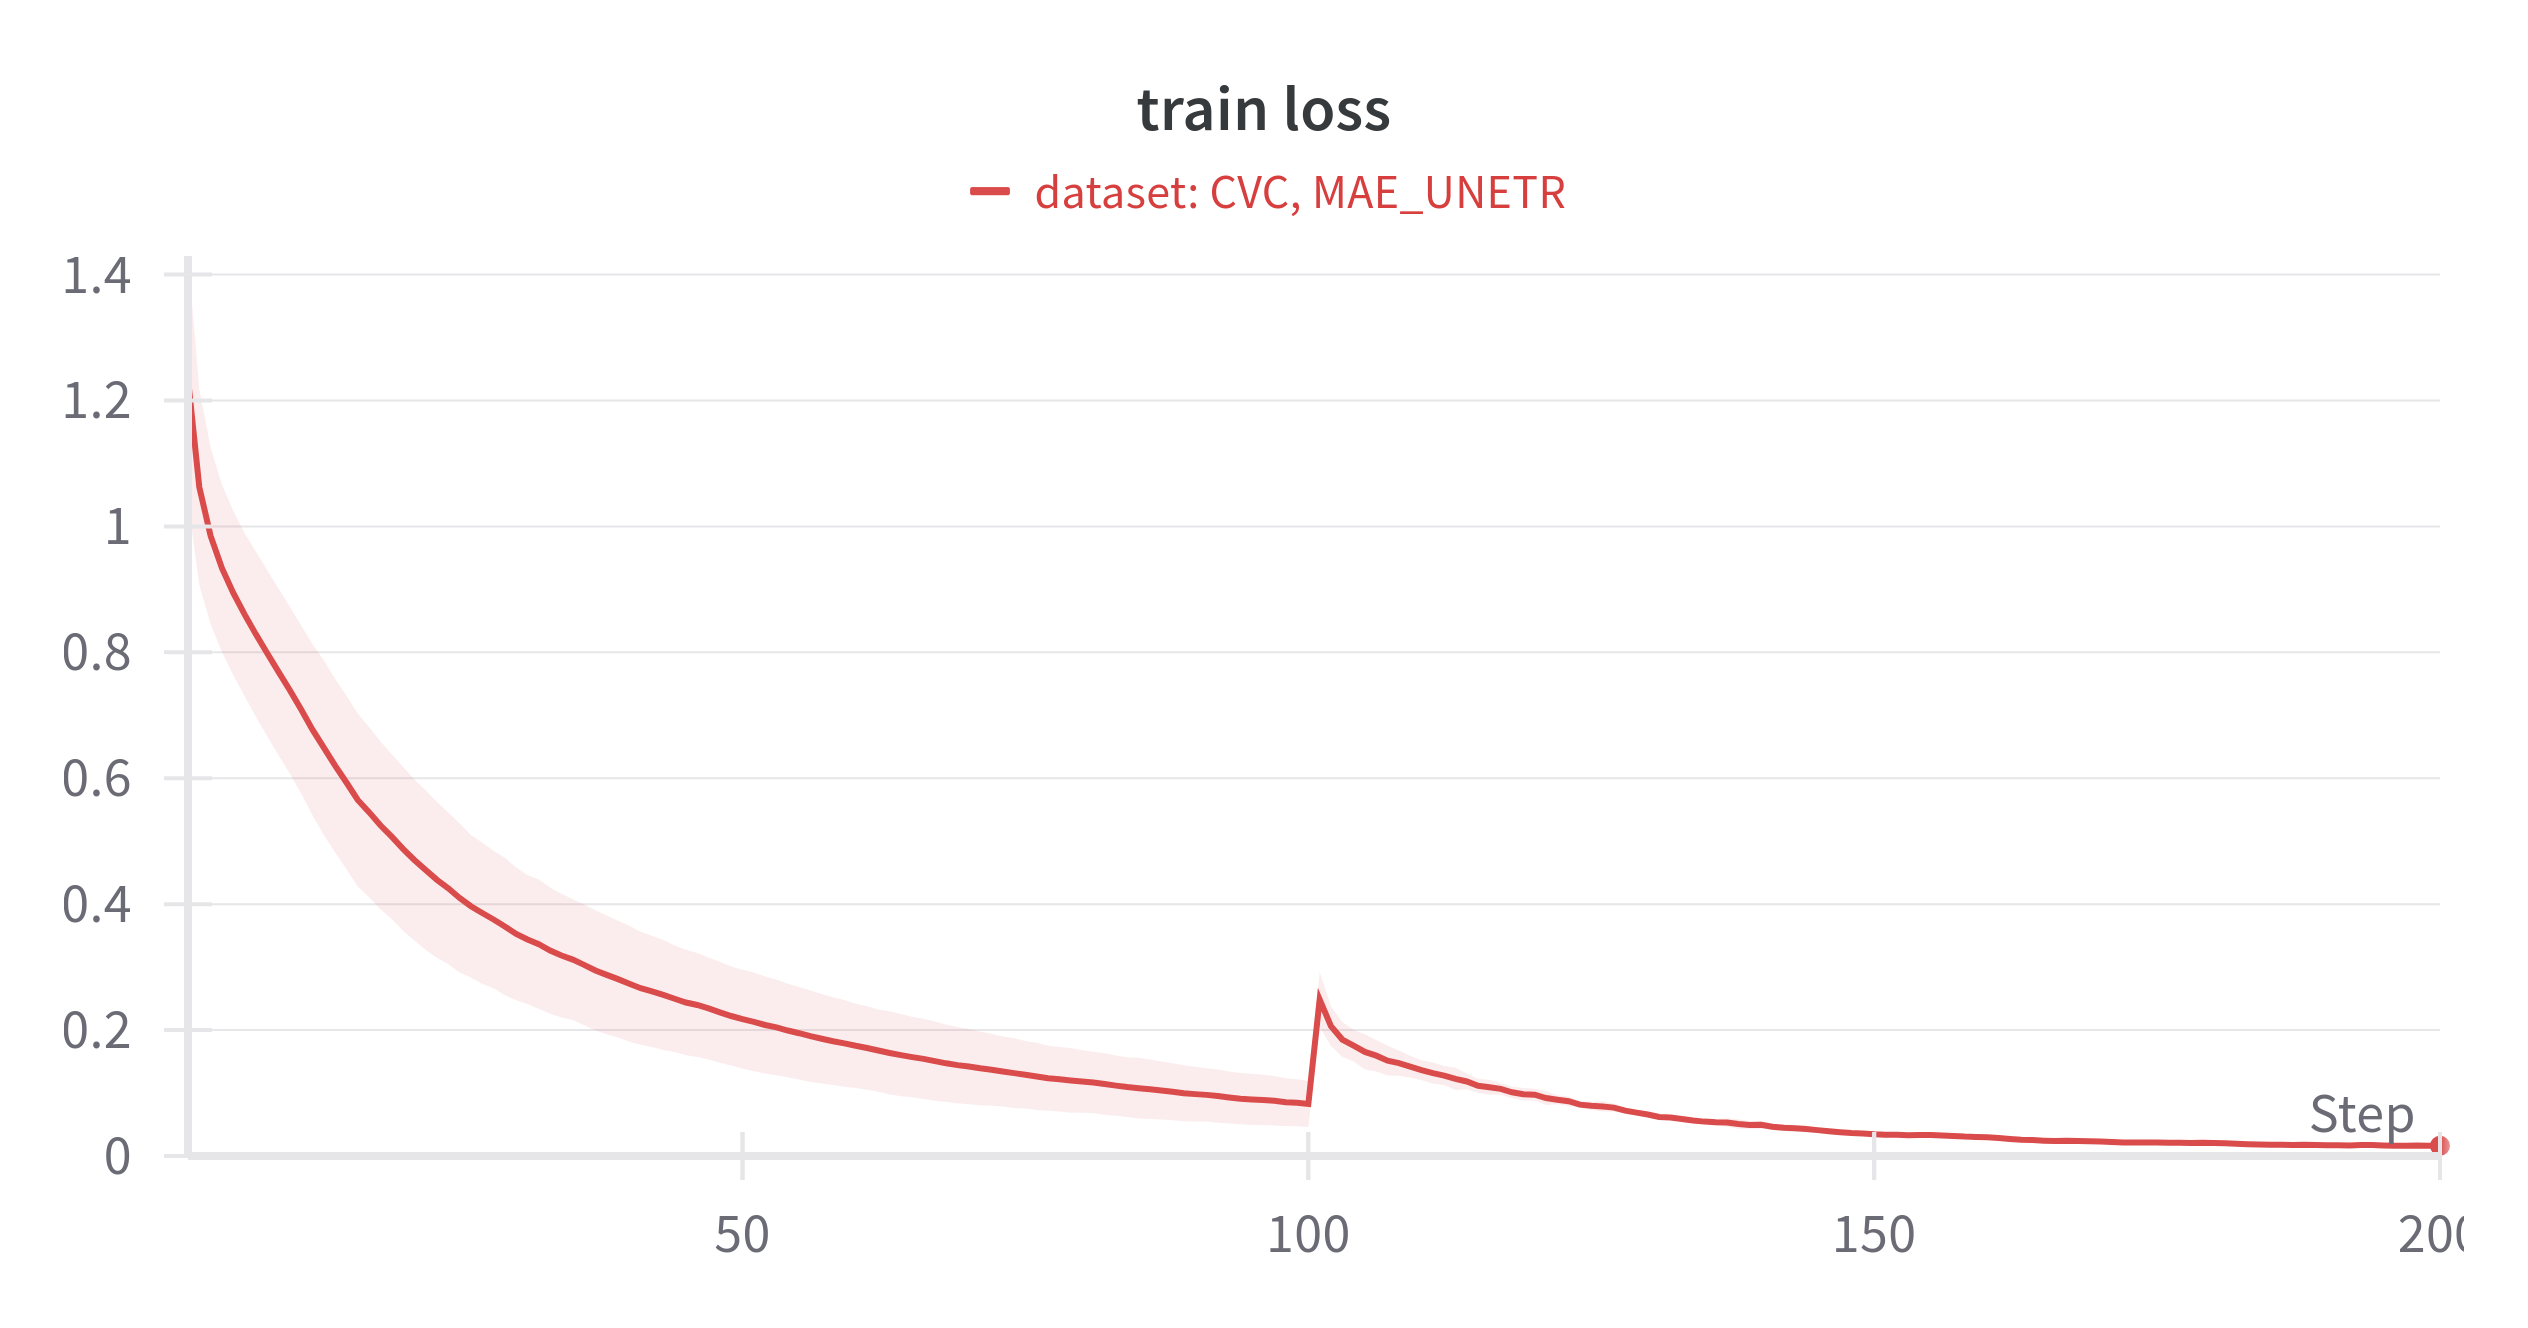
\includegraphics[width=\linewidth]{images/mae_unetr/cvc_train_loss.png}
        \caption{Training Loss - CVC}
    \end{subfigure}
    \hfill
    \begin{subfigure}{0.45\textwidth}
        \centering
        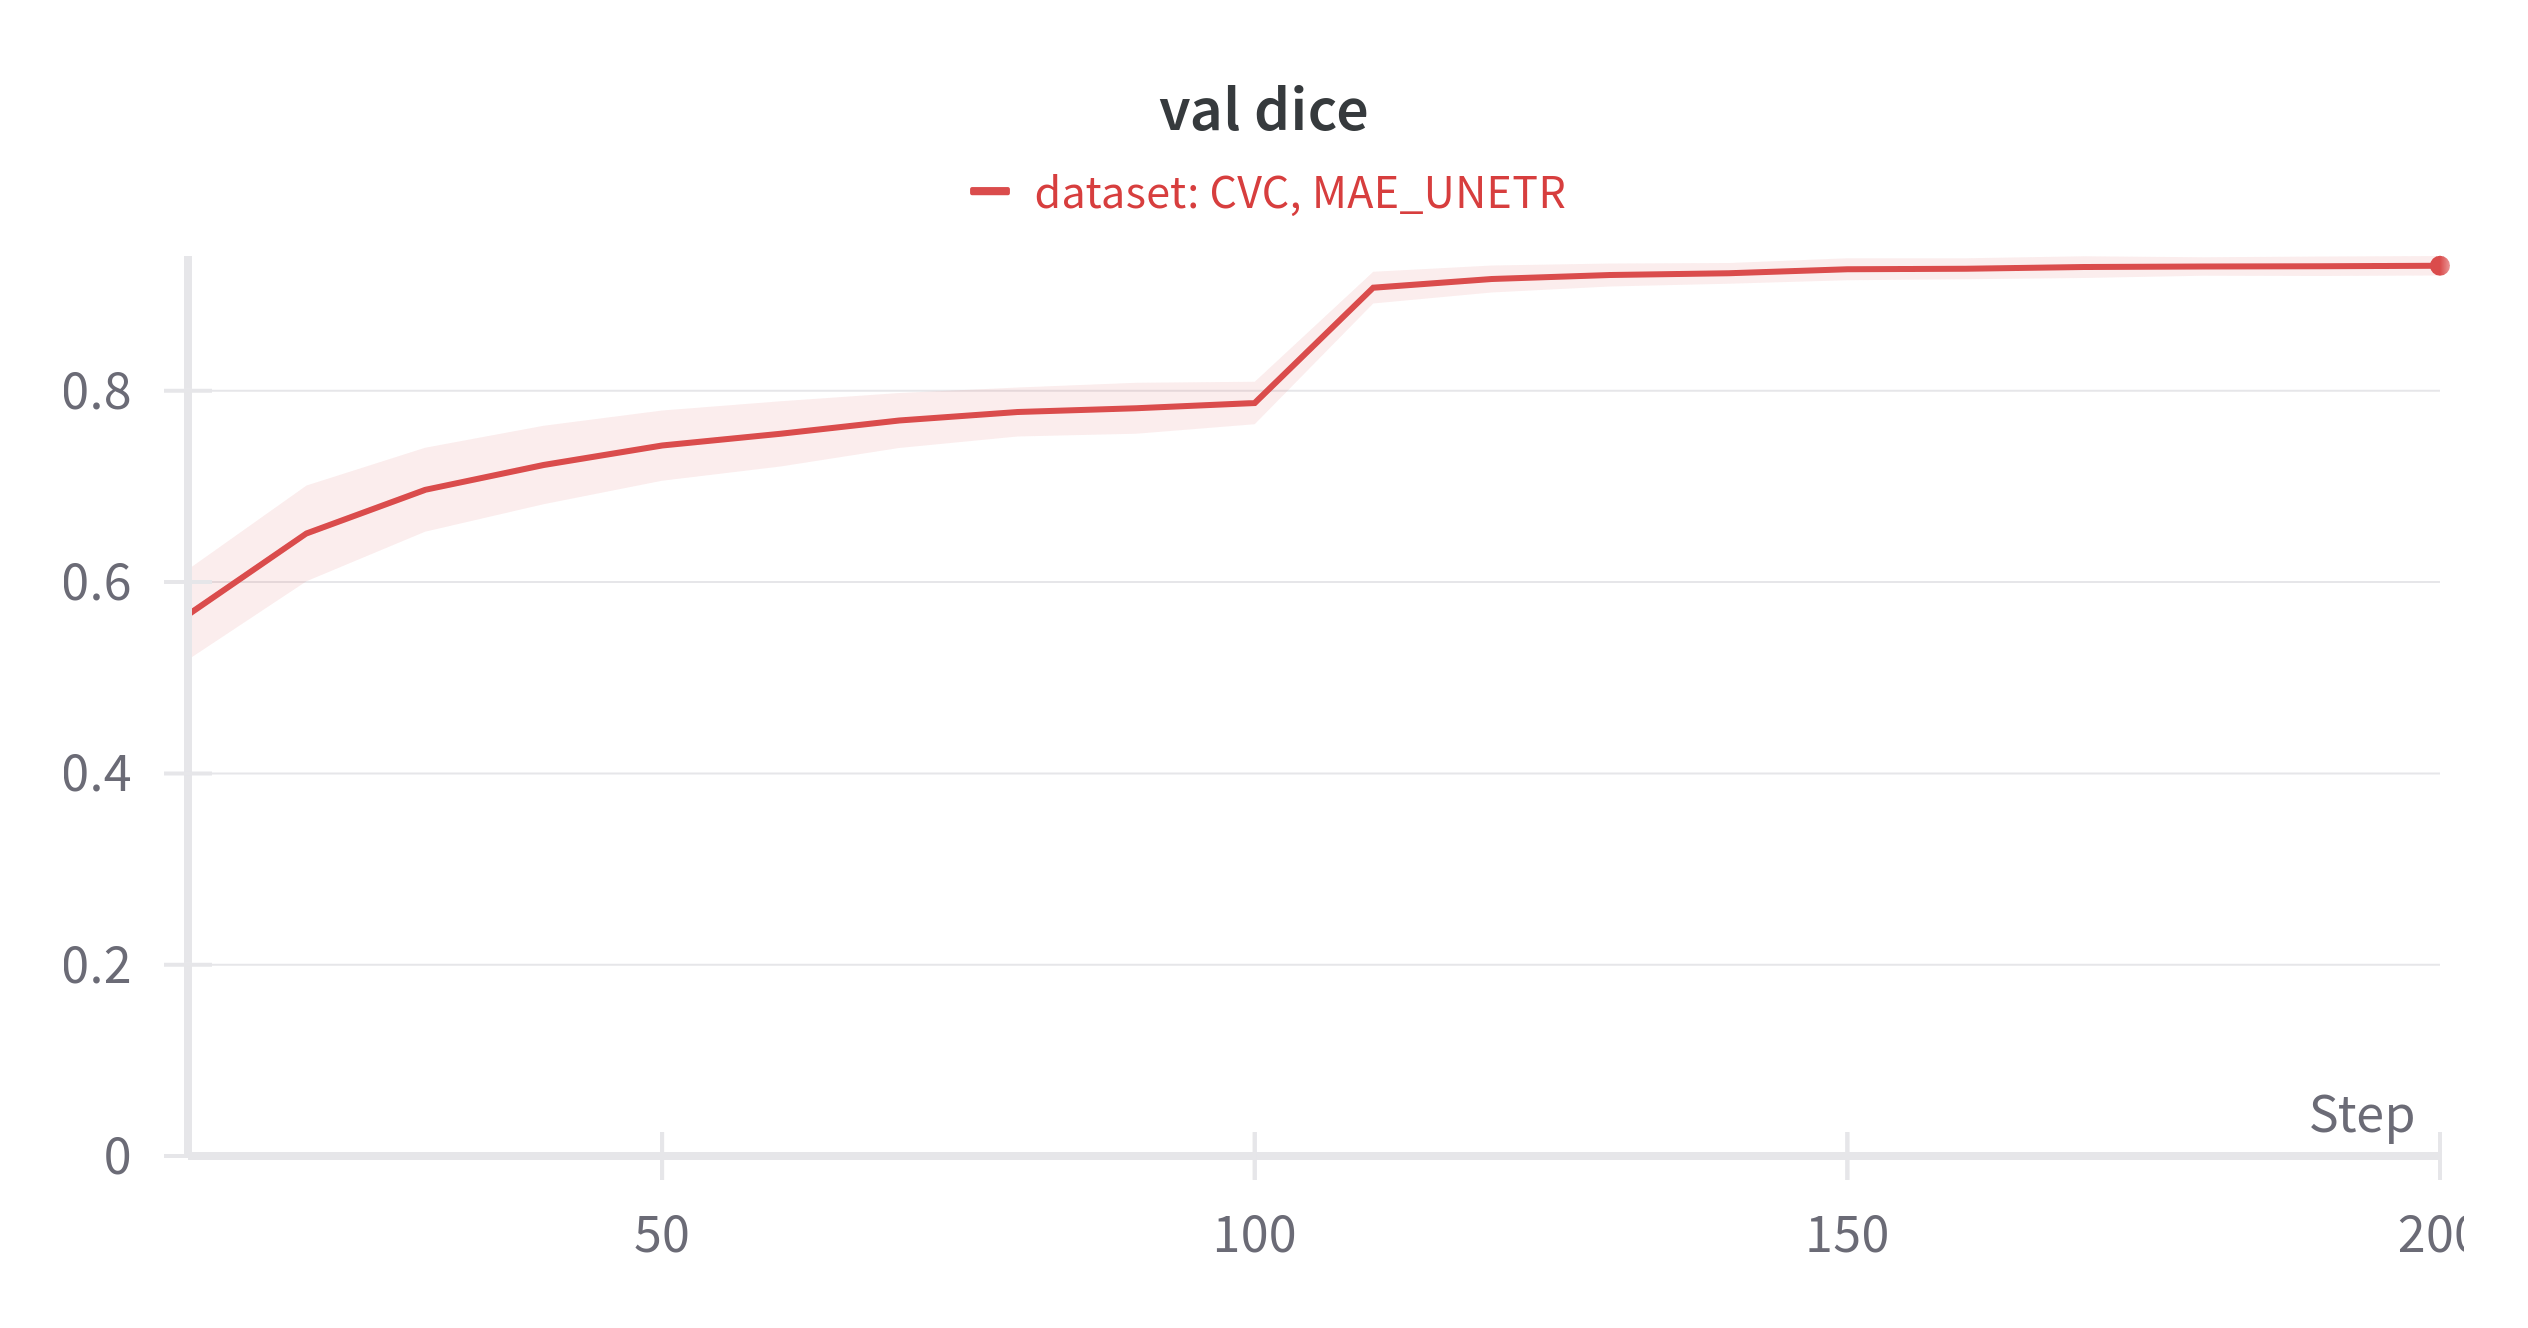
\includegraphics[width=\linewidth]{images/mae_unetr/cvc_val_dice.png}
        \caption{Validation Dice - CVC}
    \end{subfigure}
    
    \begin{subfigure}{0.45\textwidth}
        \centering
        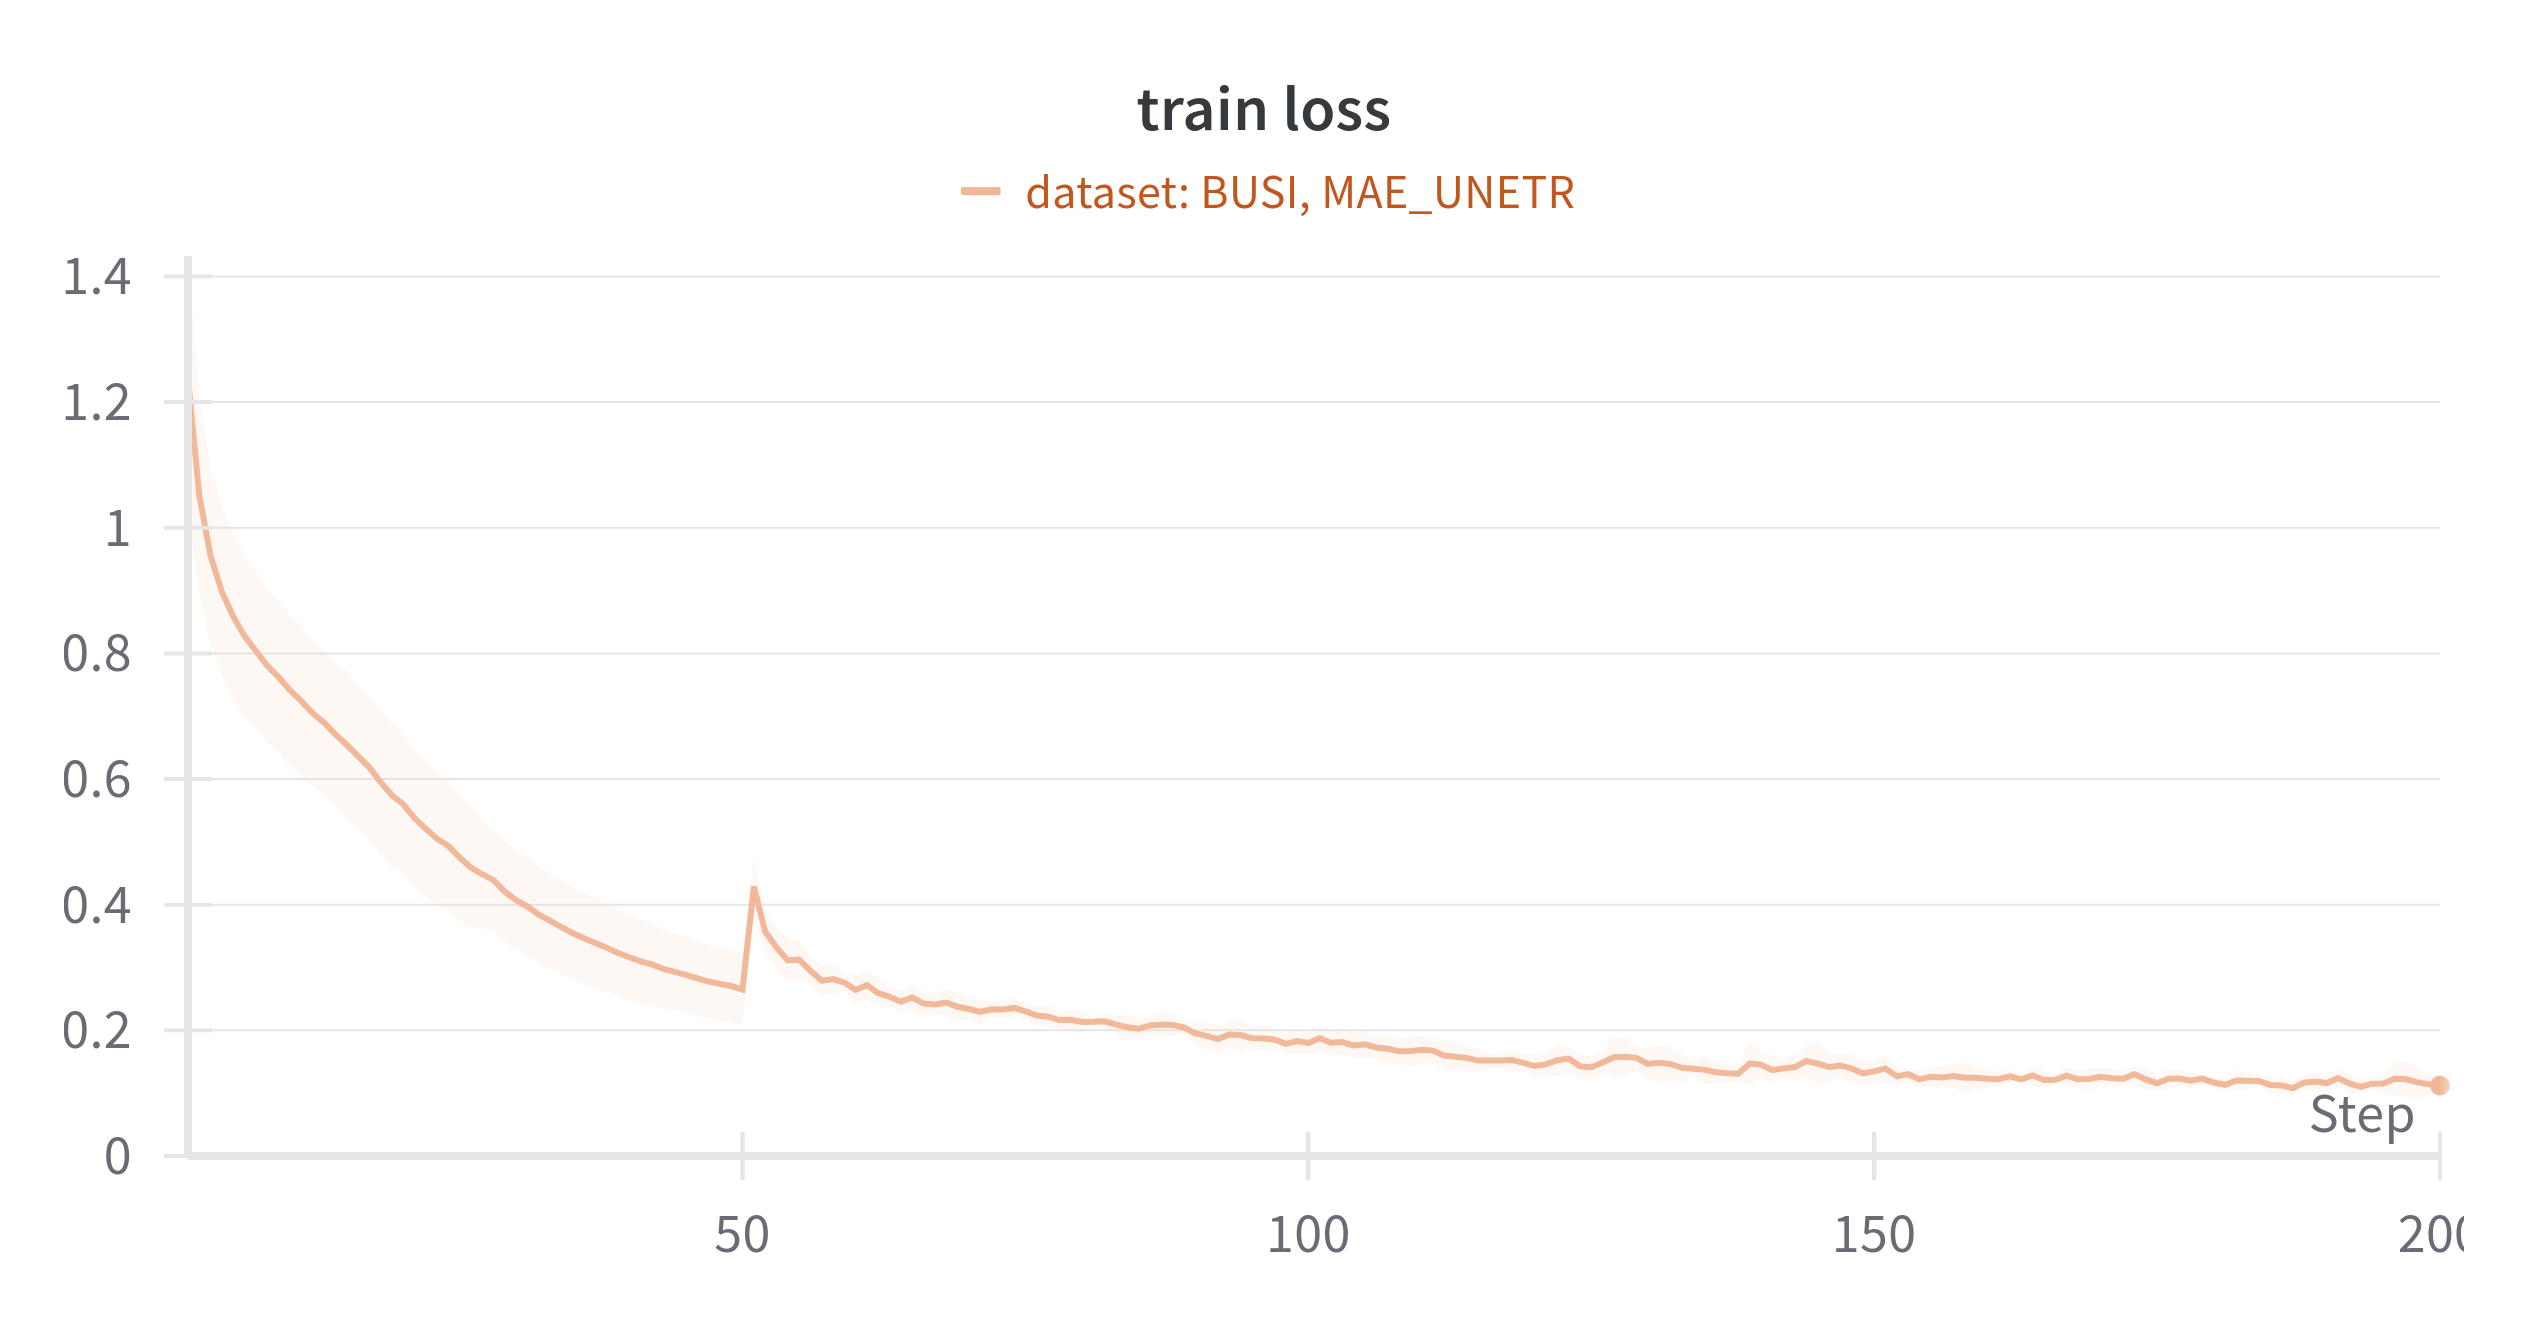
\includegraphics[width=\linewidth]{images/mae_unetr/busi_train_loss.png}
        \caption{Training Loss - BUSI}
    \end{subfigure}
    \hfill
    \begin{subfigure}{0.45\textwidth}
        \centering
        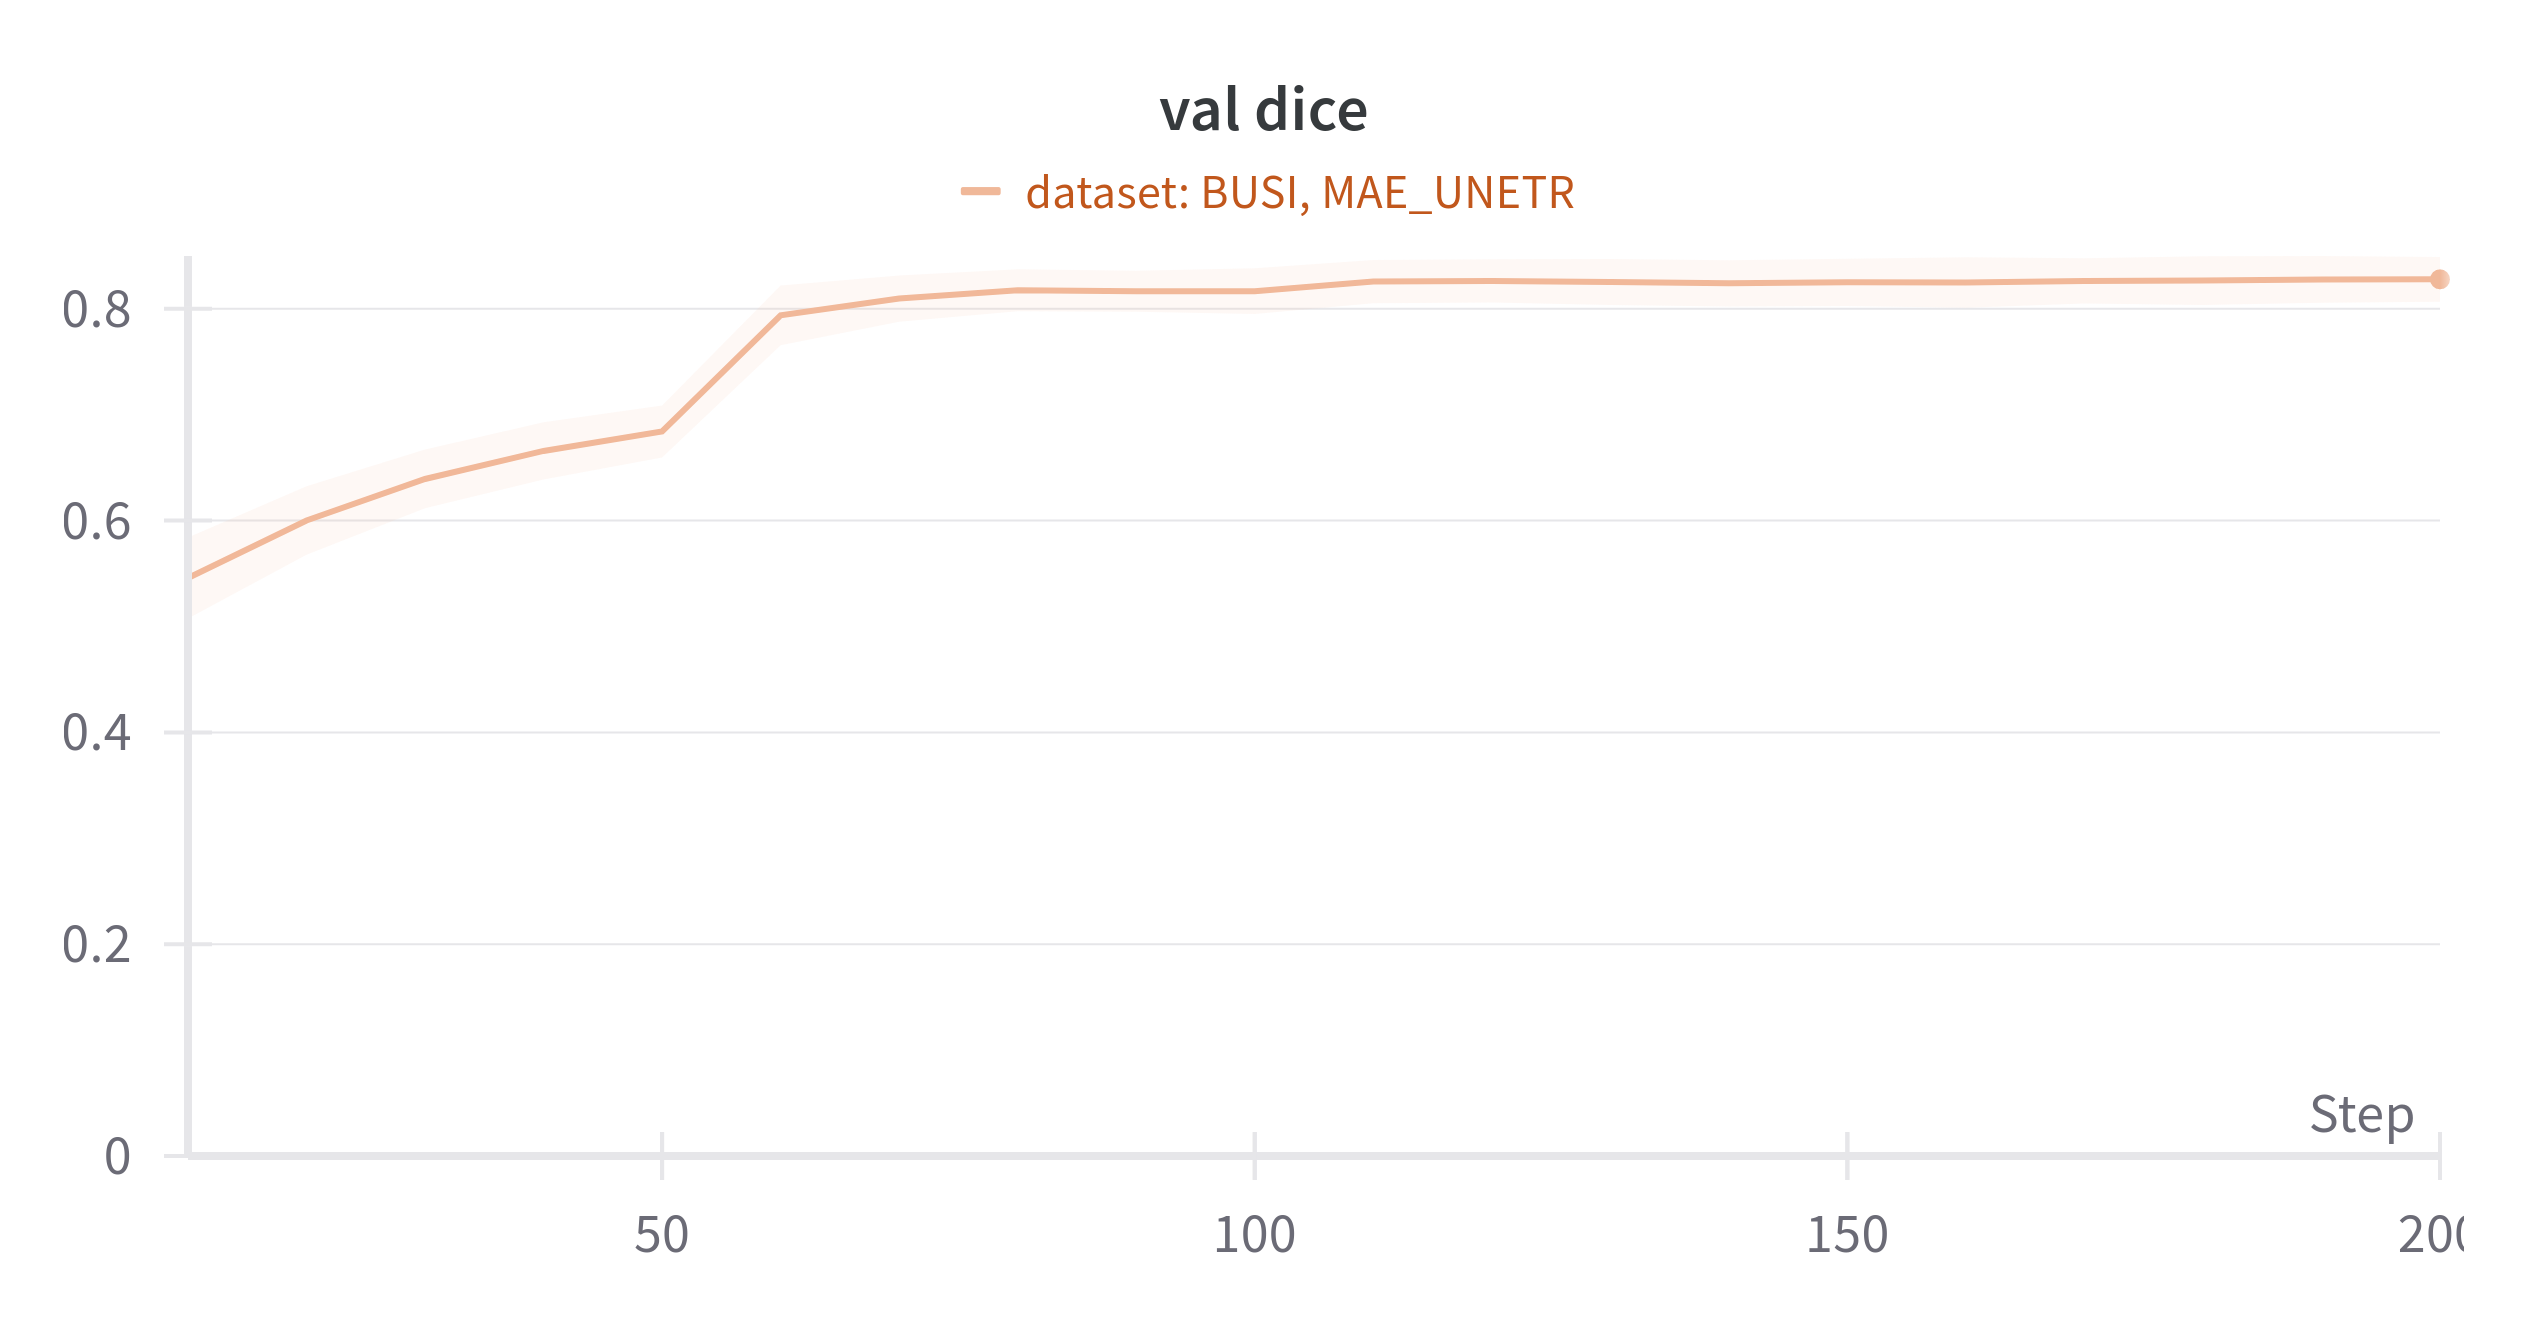
\includegraphics[width=\linewidth]{images/mae_unetr/busi_val_dice.png}
        \caption{Validation Dice - BUSI}
    \end{subfigure}
    
    \begin{subfigure}{0.45\textwidth}
        \centering
        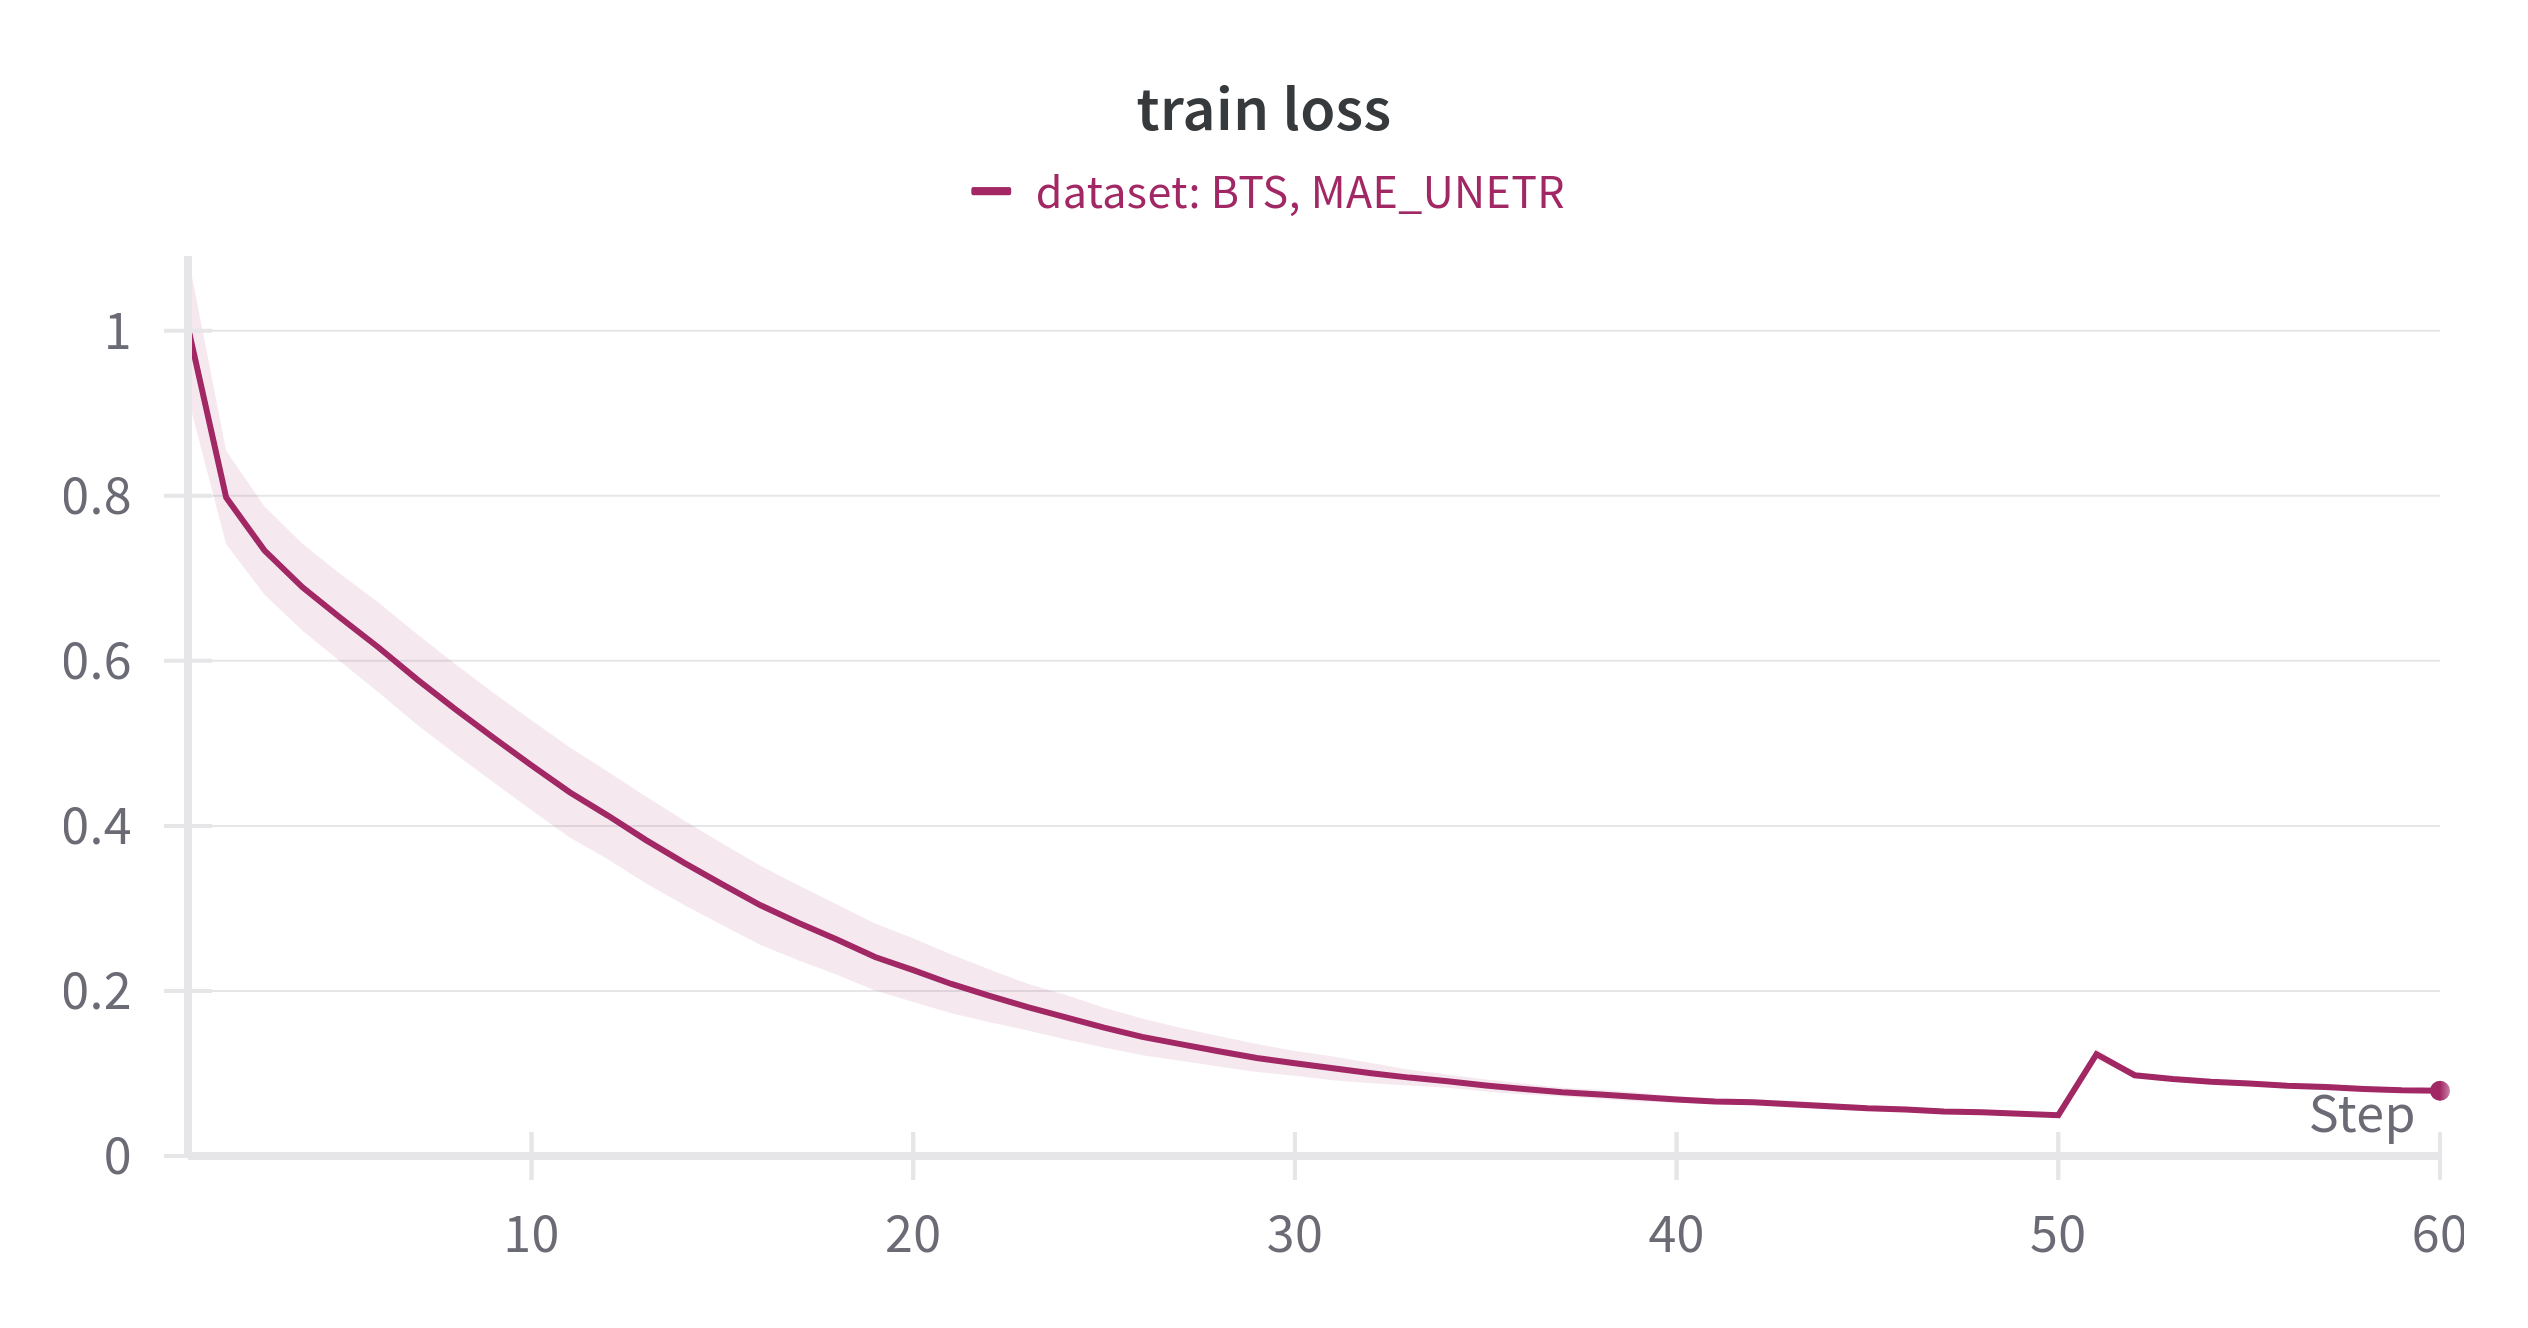
\includegraphics[width=\linewidth]{images/mae_unetr/bts_train_loss.png}
        \caption{Training Loss - BTS}
    \end{subfigure}
    \hfill
    \begin{subfigure}{0.45\textwidth}
        \centering
        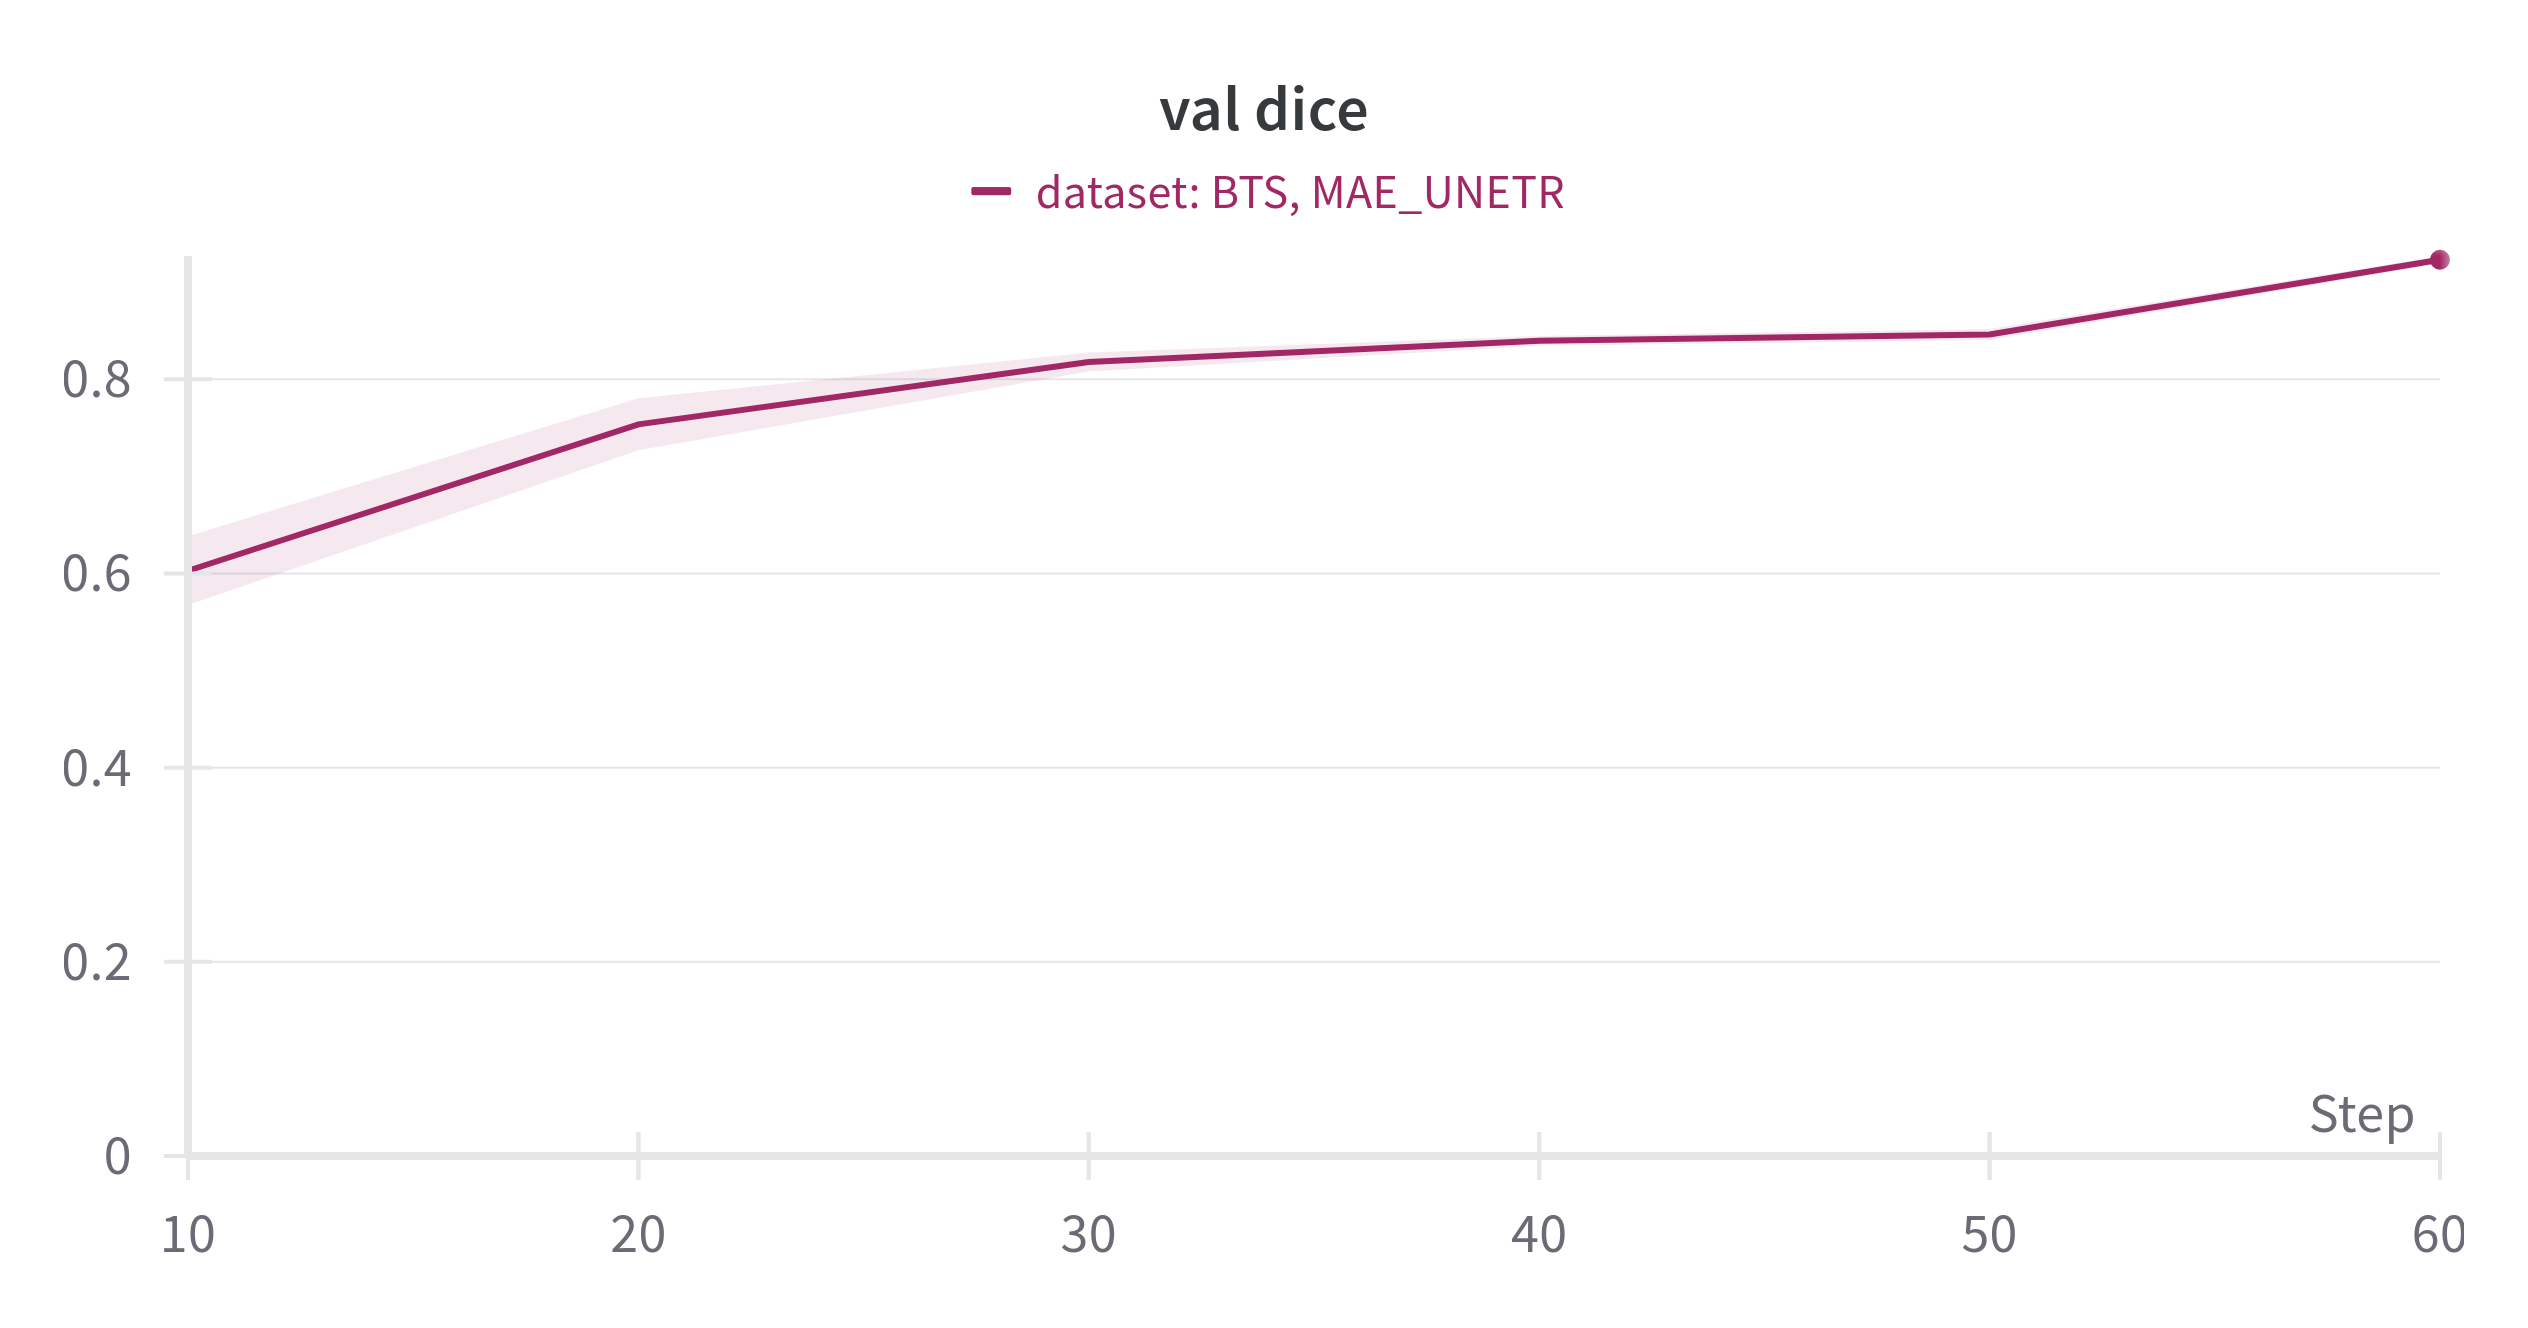
\includegraphics[width=\linewidth]{images/mae_unetr/bts_val_dice.png}
        \caption{Validation Dice - BTS}
    \end{subfigure}
    
    \caption{Training and Validation Metrics for Each Dataset}
    \label{fig:training-validation-mae}
\end{figure}

As you can see from the figure \ref{fig:training-validation-mae}, which shows the training losses and the validations, taking into account the average and standard deviation for the 5 runs that were done in the training (see Section 5.1 for details), all the losses manage to converge with the number of established epochs, and reporting a decreasing standard deviation, indicating that repeated experiments are stable.\\In general, also validation dices for the three datasets exhibit this behaviour, an indication of stability in the training experiments.

\subsubsection{Unet}
The training phase for the U-Net architecture encompasses a singular yet comprehensive approach, where the entire network is iteratively trained on the dataset of interest. Unlike the multi-phase training regimen observed in the Mae+UNETR network, the U-Net training entails a straightforward process focused on maximizing the model's predictive capabilities.\\

Throughout the training phase, a constant learning rate is maintained, fostering stable convergence and facilitating efficient parameter updates. This simplicity in learning rate management streamlines the training process, ensuring consistent model refinement and adaptation to diverse input data distributions.\\

Additionally, dropout regularization is employed within the U-Net architecture to mitigate overfitting and enhance model generalization. By selectively dropping units during training, dropout encourages the network to learn robust features and prevent reliance on specific nodes, thereby enhancing its capacity to generalize across unseen data instances.\\

Moreover, for the training of the U-Net, a batch size of 16 was employed. This moderate batch size strikes a balance between computational efficiency and model convergence, facilitating effective parameter updates while efficiently utilizing available computational resources.

\begin{table}[H]
\begin{center}
\begin{tabular}{p{2cm}cc}
\textbf{Dataset} & \textbf{Learning Rate} & \textbf{Epochs} \\
CVC  & 1e-4 & 100 \\
BUSI & 1e-4  & 400 \\
BTS  & 1e-3  & 100 \\
\end{tabular}
\caption{Training Parameters for Each Dataset}
% \label{tab:dataset-parameters}
\end{center}
\end{table}

\begin{figure}[h]
    \centering
    \begin{subfigure}{0.45\textwidth}
        \centering
        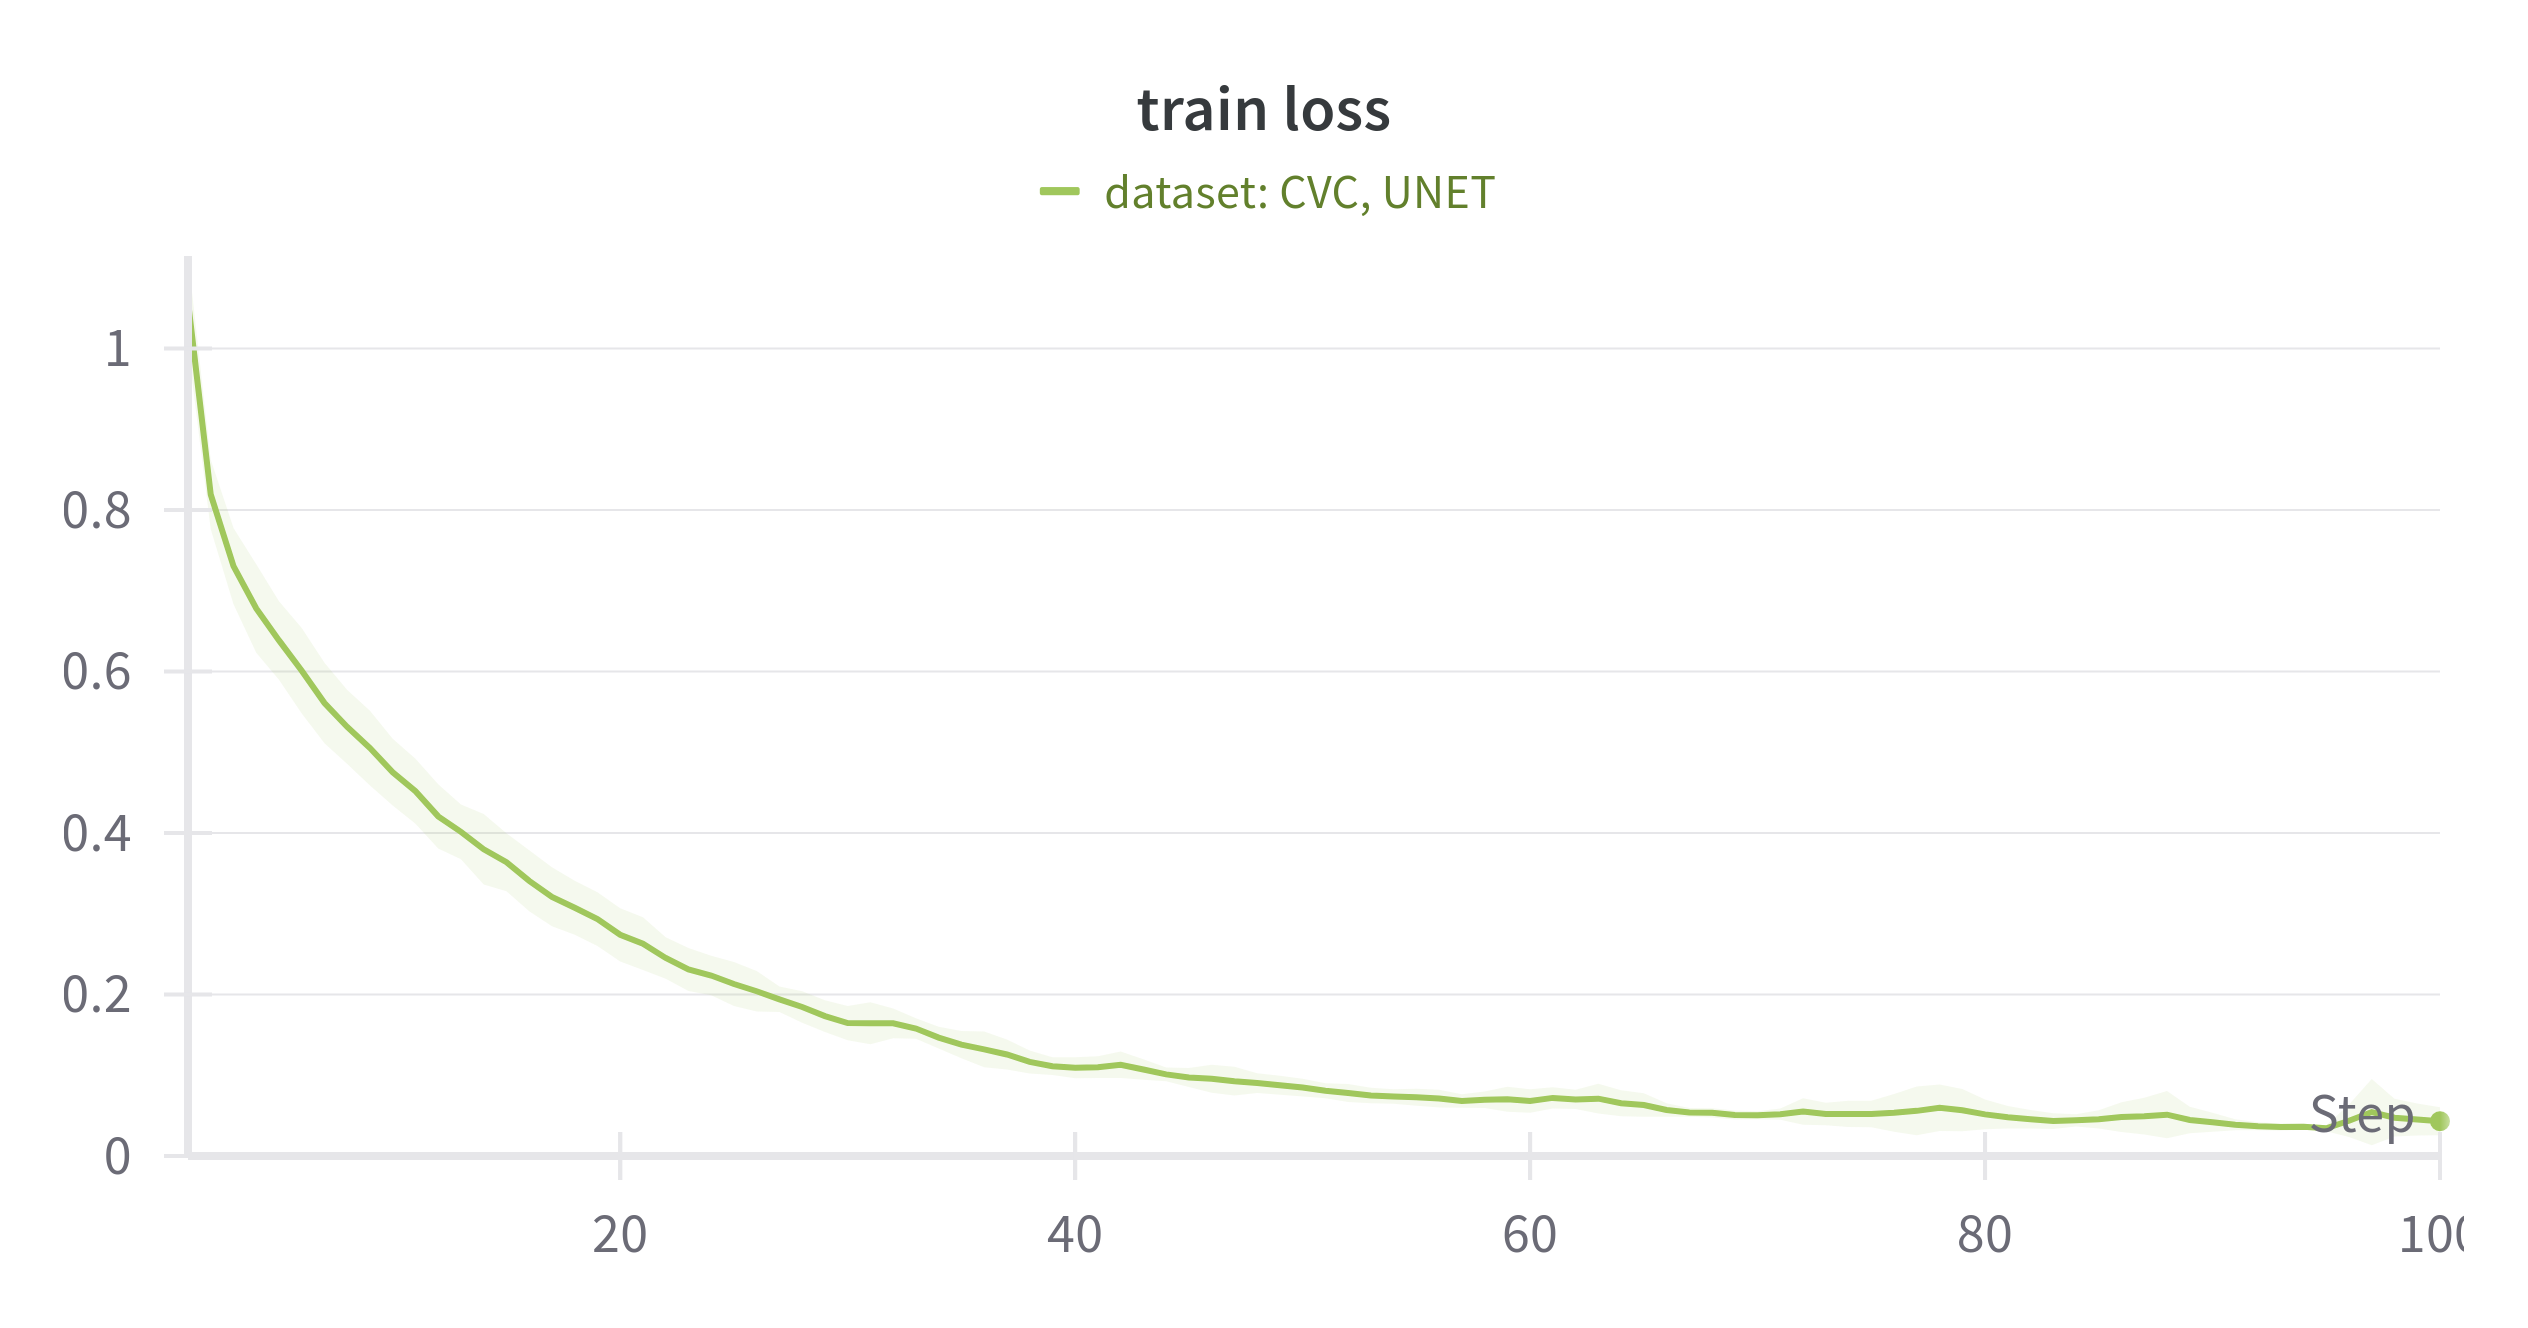
\includegraphics[width=\linewidth]{images/unet/cvc_train_loss.png}
        \caption{Training Loss - CVC}
    \end{subfigure}
    \hfill
    \begin{subfigure}{0.45\textwidth}
        \centering
        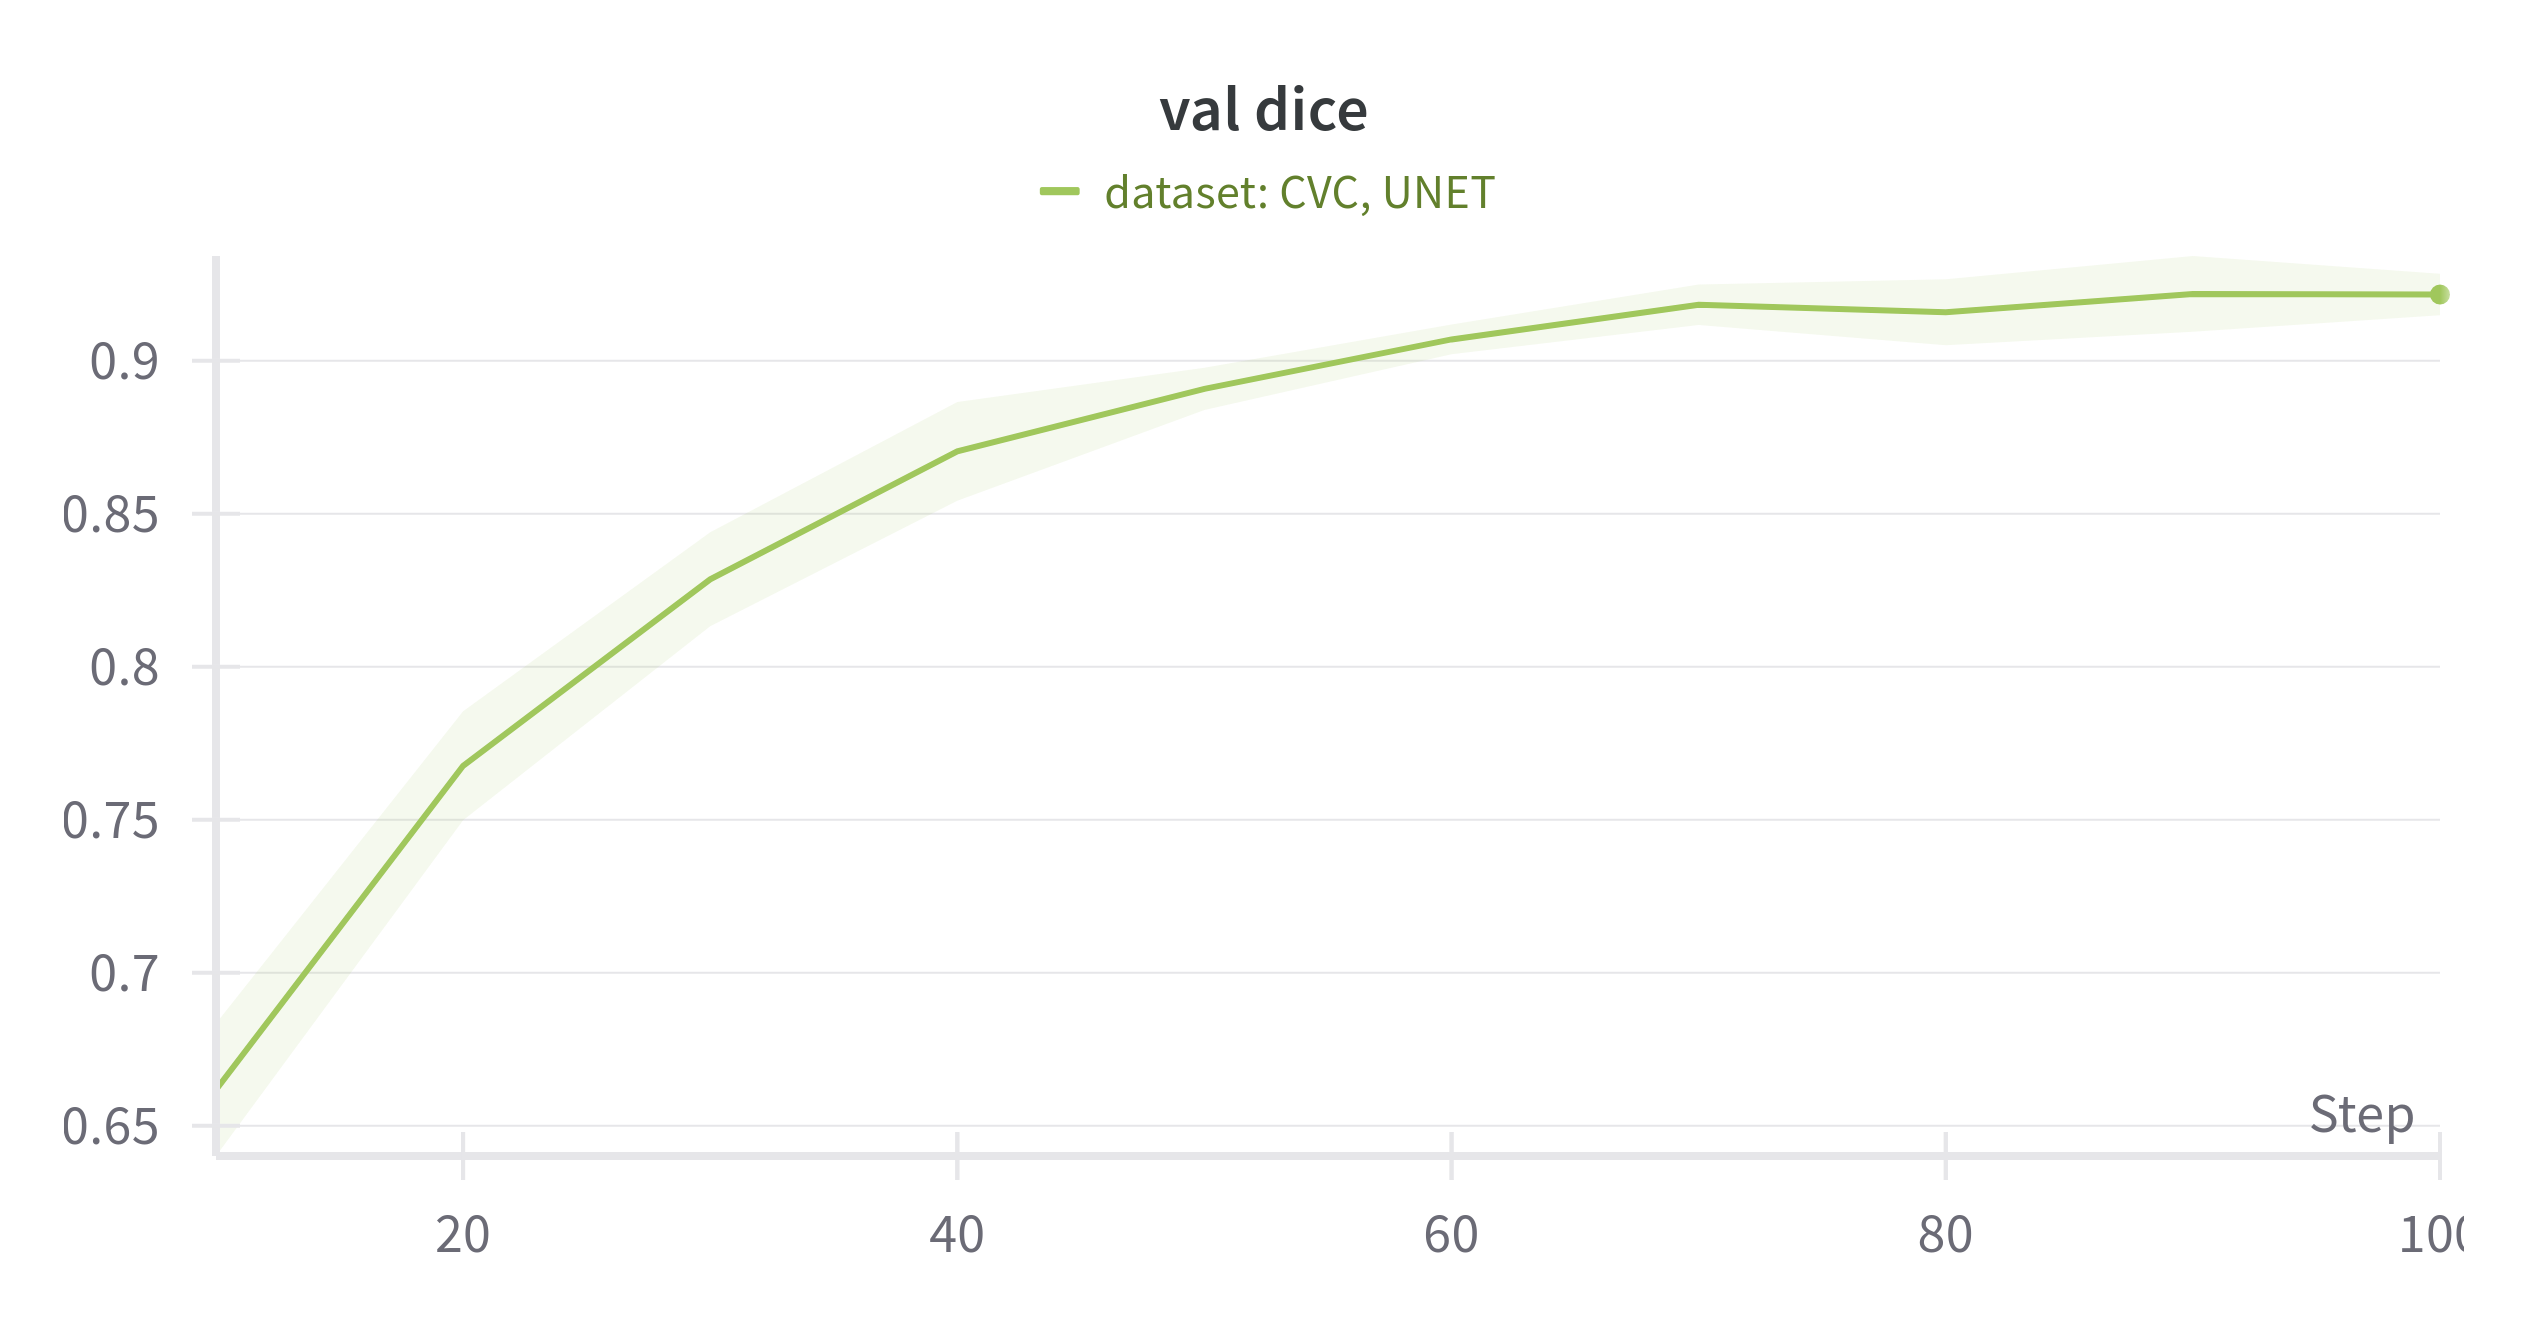
\includegraphics[width=\linewidth]{images/unet/cvc_val_dice.png}
        \caption{Validation Dice - CVC}
    \end{subfigure}
    
    \begin{subfigure}{0.45\textwidth}
        \centering
        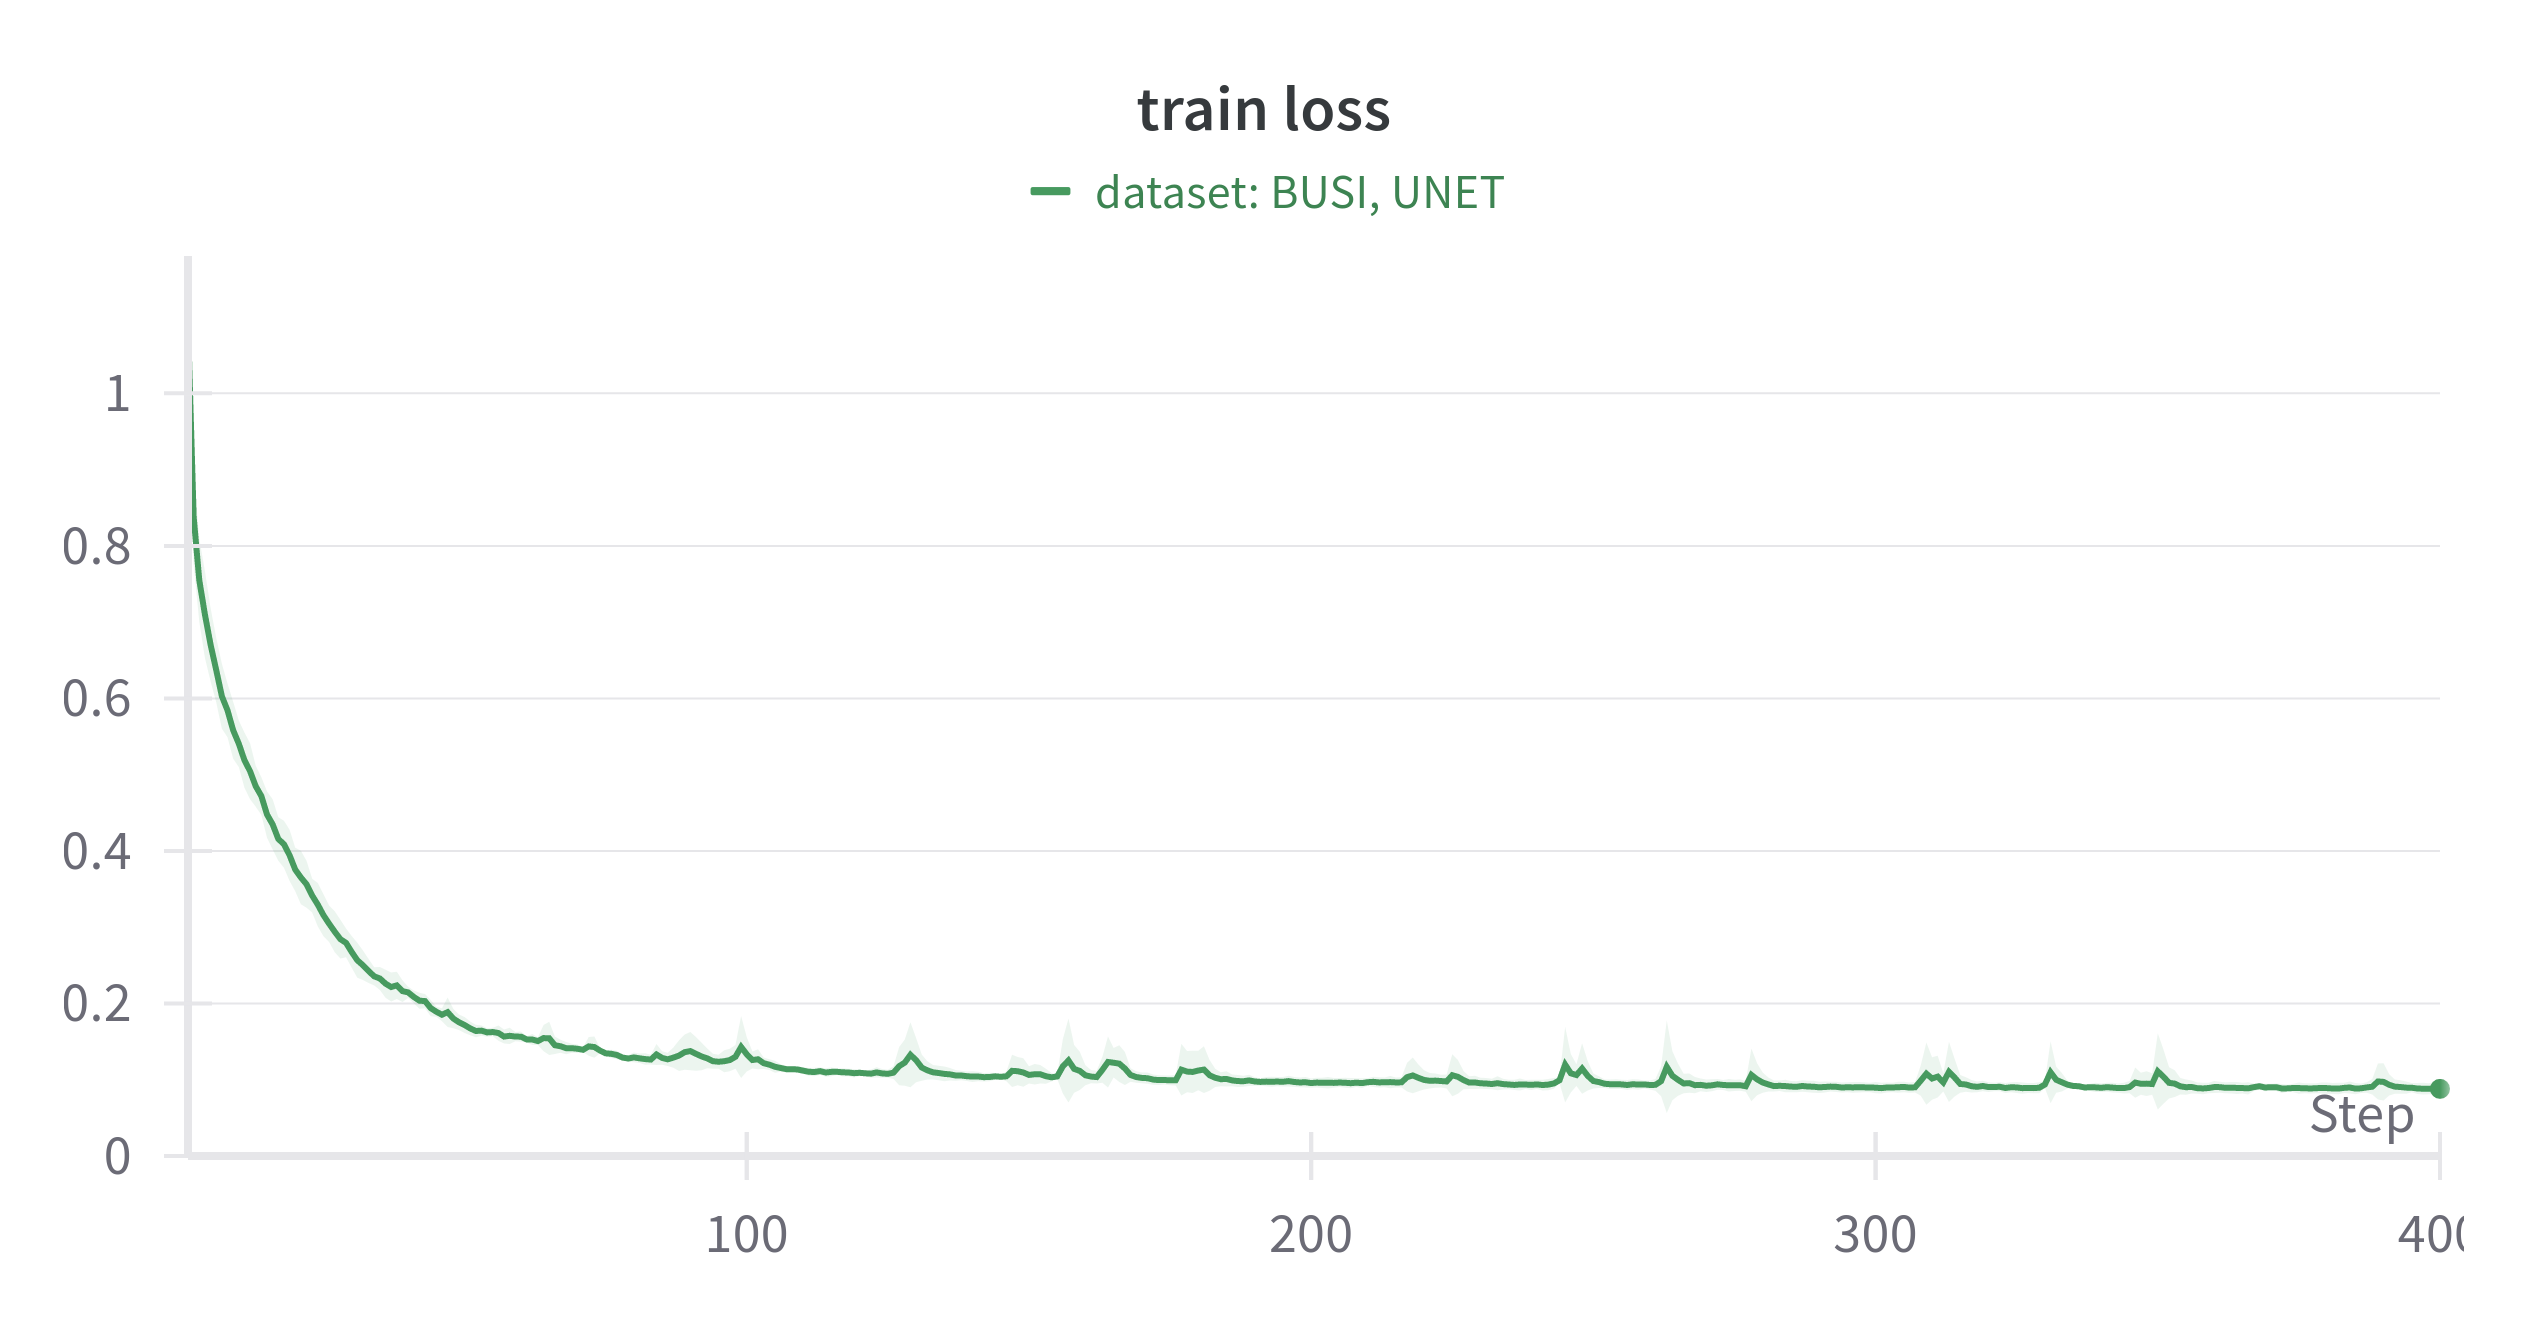
\includegraphics[width=\linewidth]{images/unet/busi_train_loss.png}
        \caption{Training Loss - BUSI}
    \end{subfigure}
    \hfill
    \begin{subfigure}{0.45\textwidth}
        \centering
        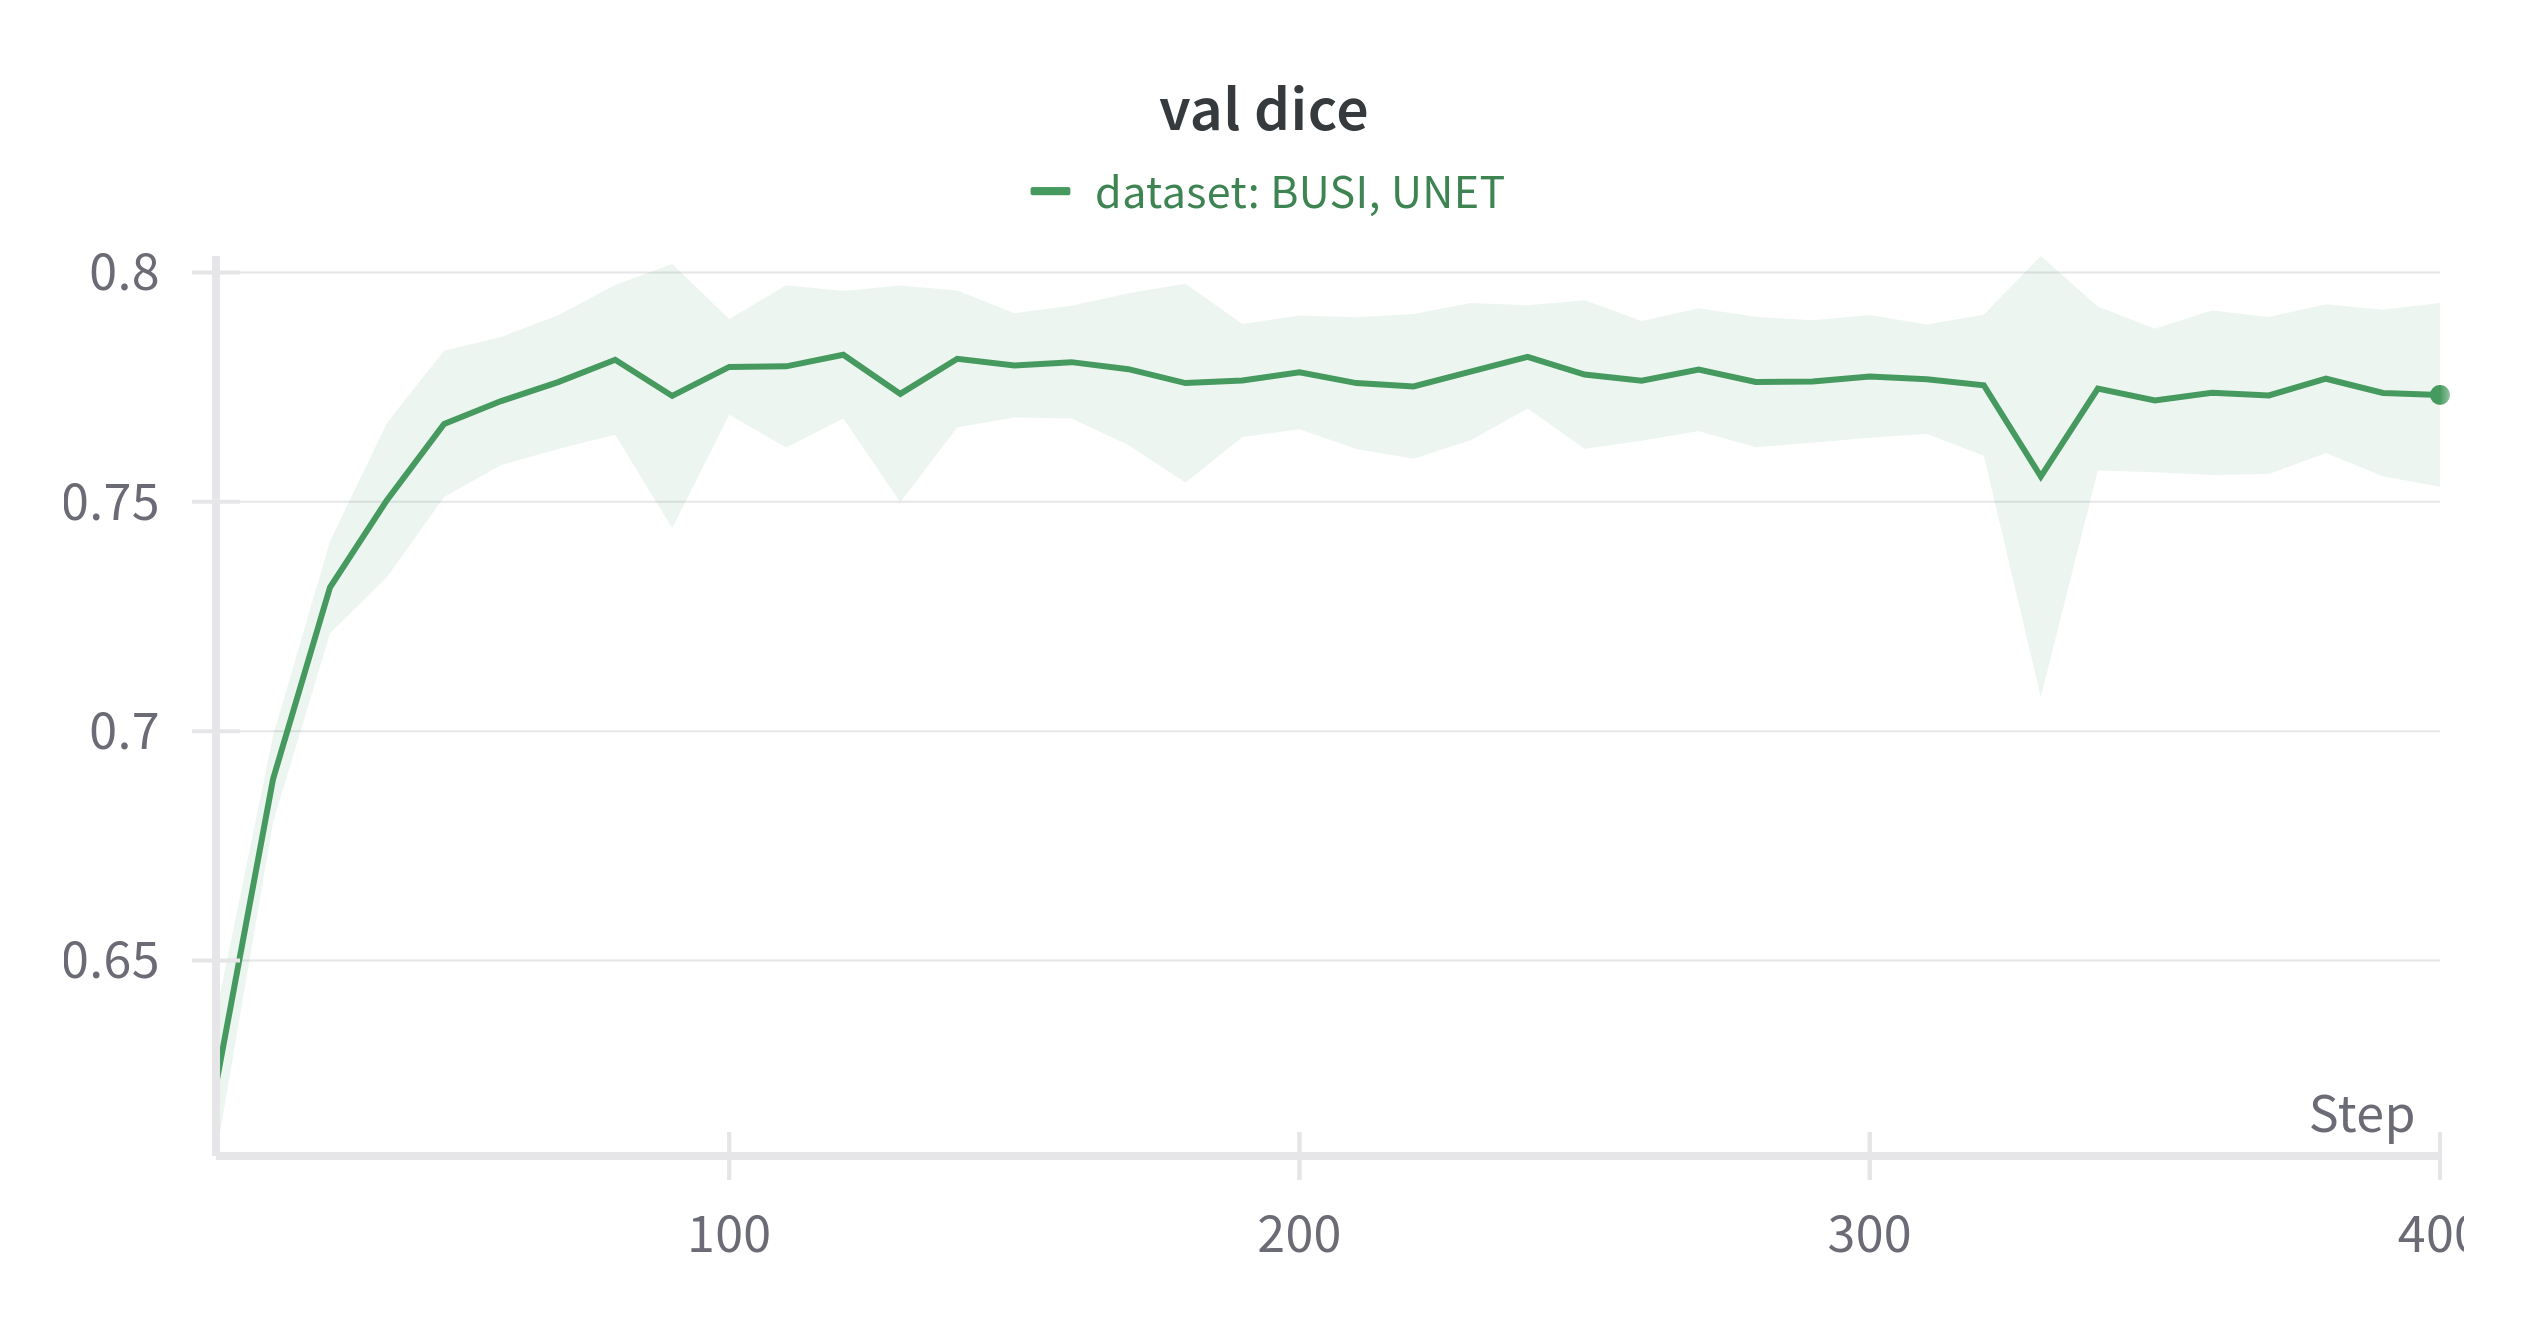
\includegraphics[width=\linewidth]{images/unet/busi_val_dice.png}
        \caption{Validation Dice - BUSI}
    \end{subfigure}
    
    \begin{subfigure}{0.45\textwidth}
        \centering
        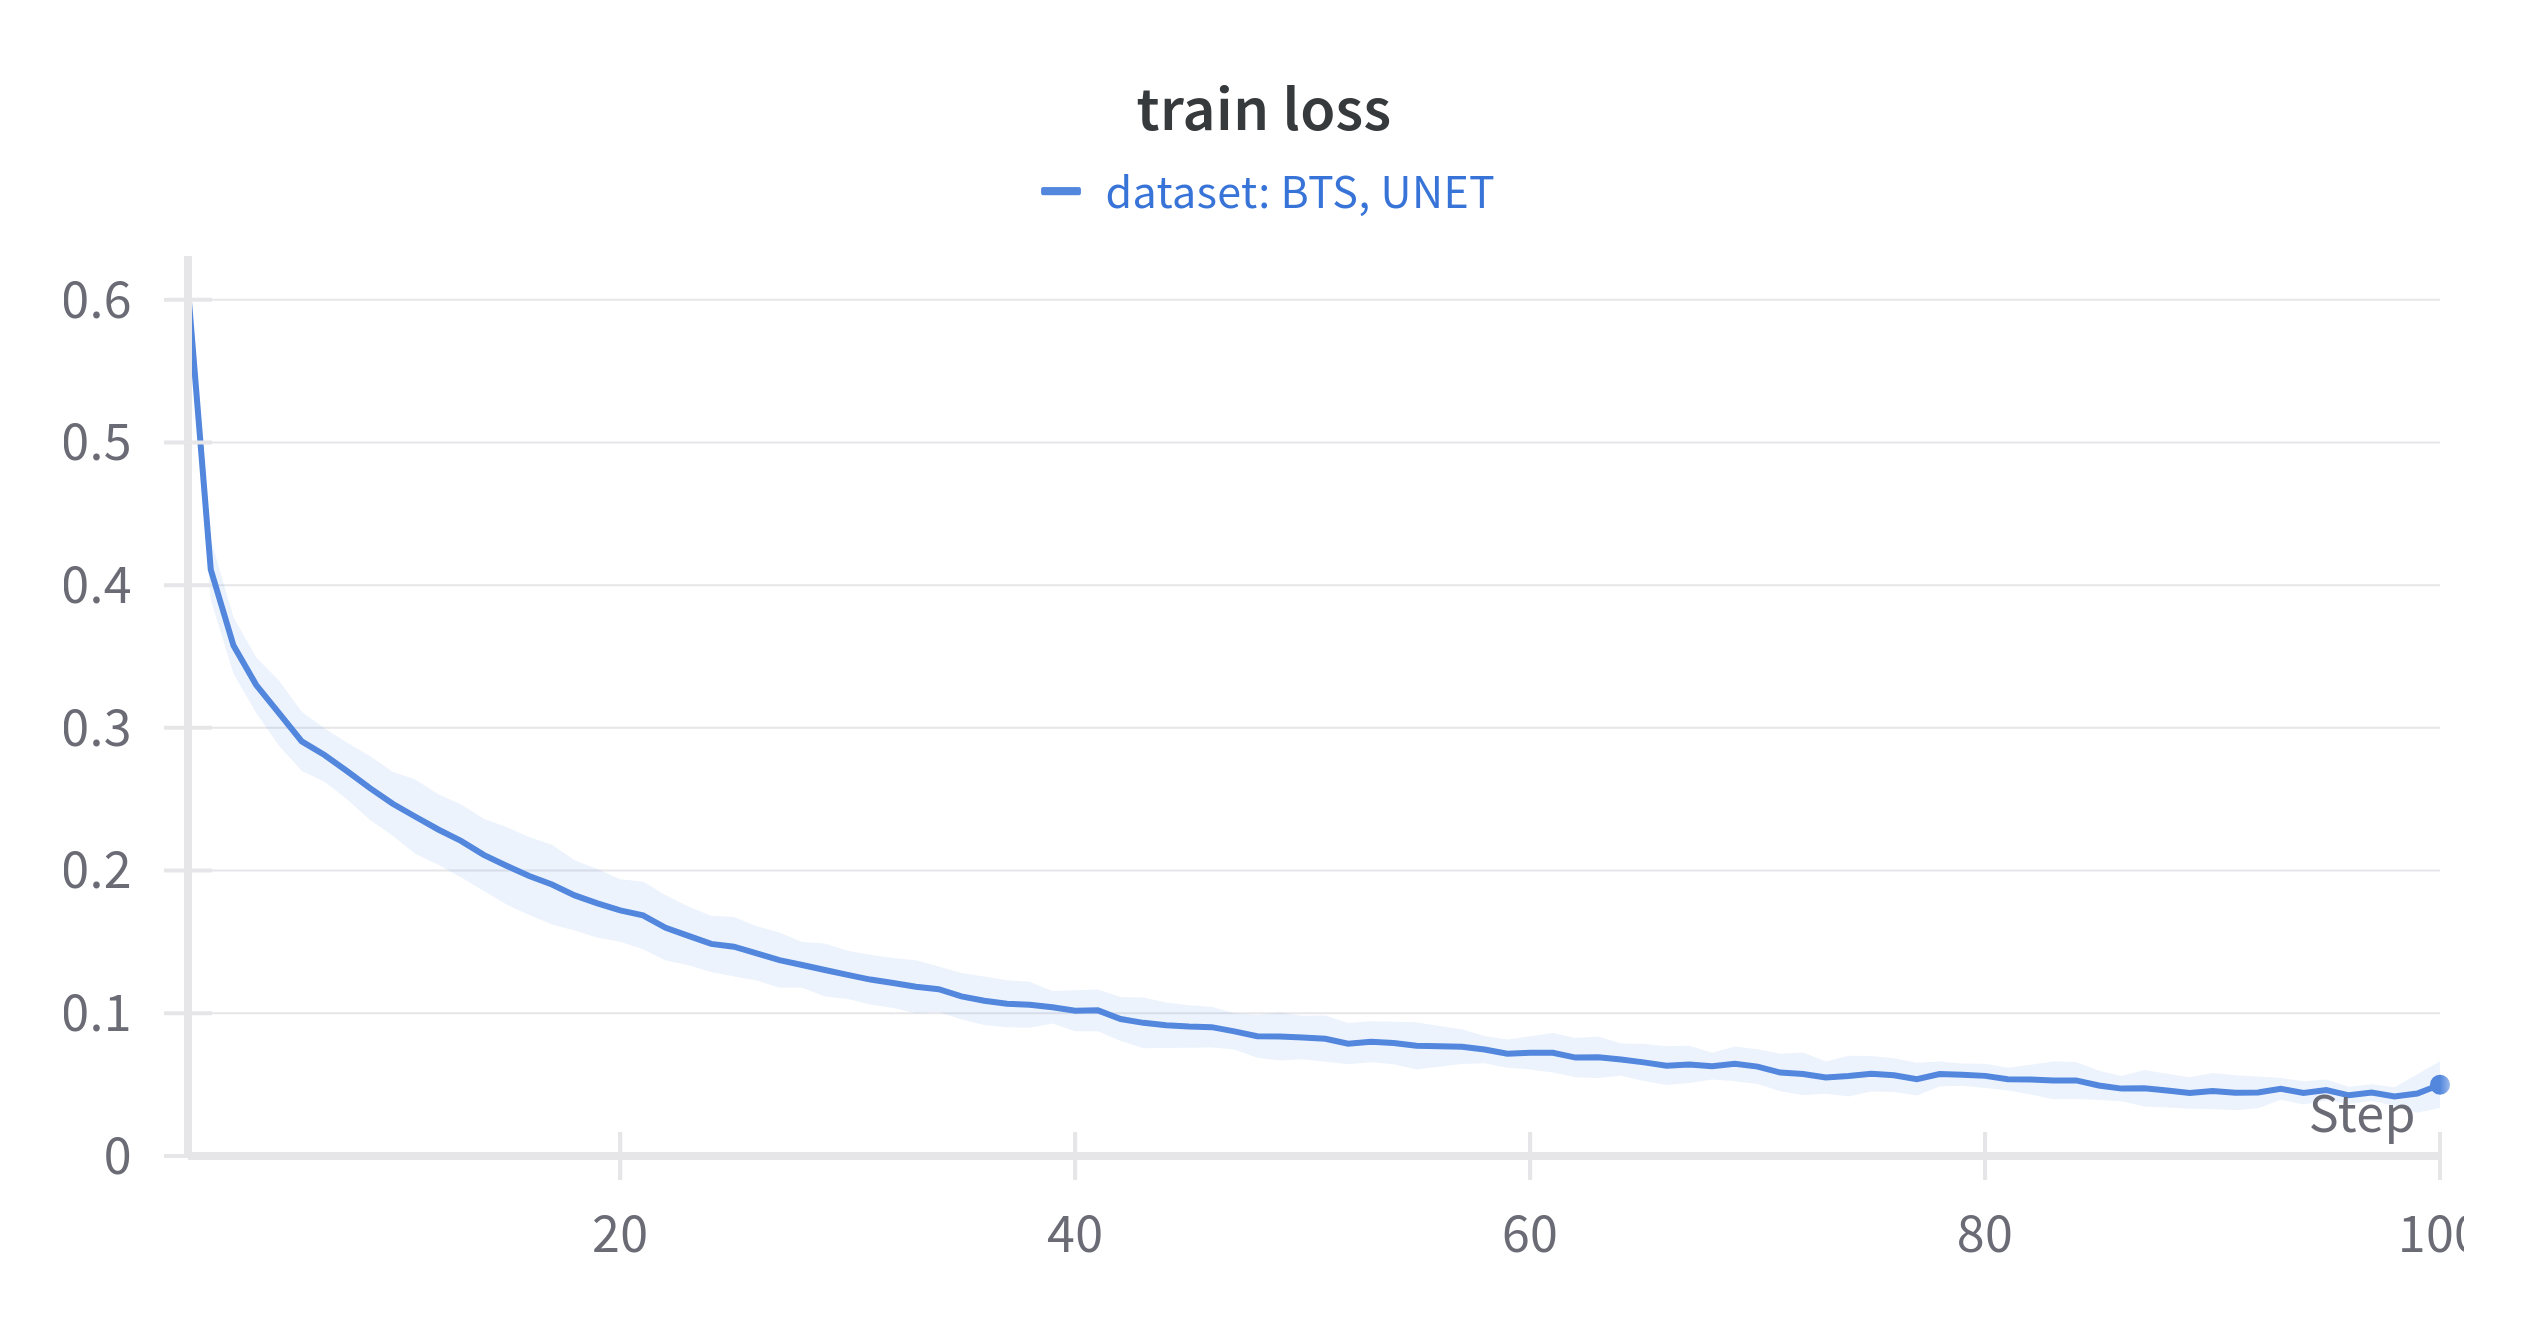
\includegraphics[width=\linewidth]{images/unet/bts_train_loss.png}
        \caption{Training Loss - BTS}
    \end{subfigure}
    \hfill
    \begin{subfigure}{0.45\textwidth}
        \centering
        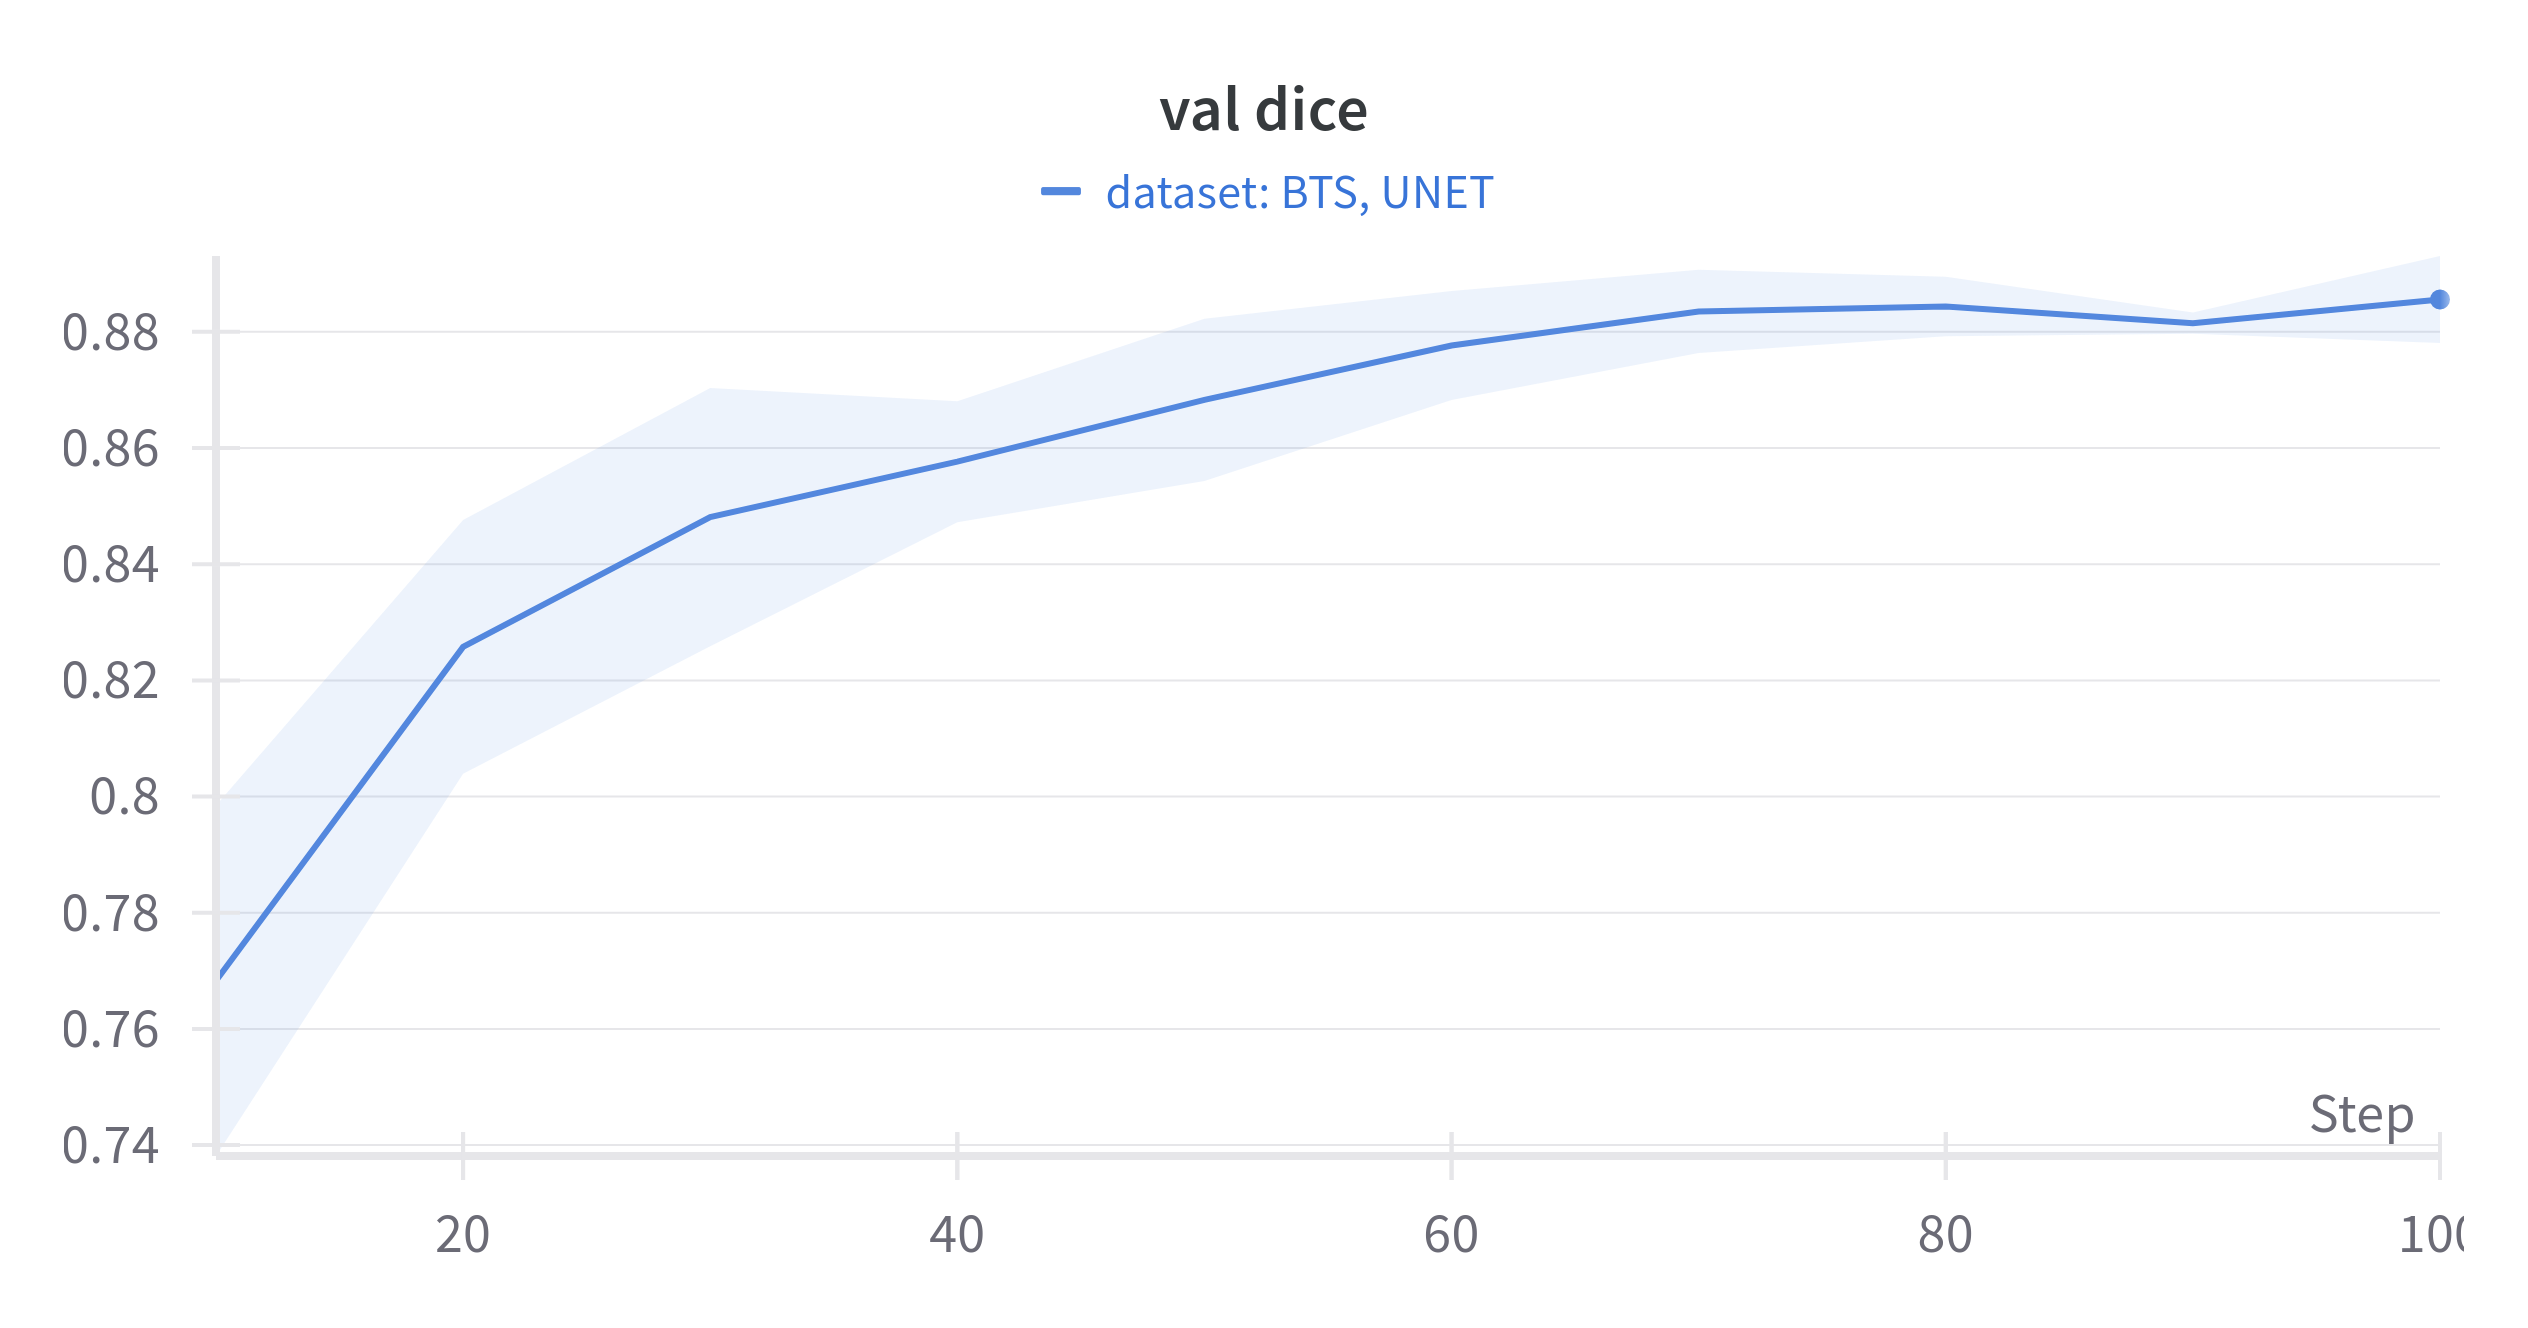
\includegraphics[width=\linewidth]{images/unet/bts_val_dice.png}
        \caption{Validation Dice - BTS}
    \end{subfigure}
    
    \caption{Training and Validation Metrics for Each Dataset}
    \label{fig:training-validation-unet}
\end{figure}

From figure \ref{fig:training-validation-unet} it can be deduced that all the losses manage to converge with the number of established epochs with a very low standard deviation from the beginning.\\ For the validation dice curves you can see that there's more variability in the standard deviations: in particular in CVC and BTS datasets, the value became lower going on with the training, while for BUSI dataset the standard deviation value remained higher, even if the value converges anyway. This could be an indication of the fact that the results are approximately stable but the variability of each run must be taken into account.


\newpage
% To conduct a thorough evaluation, we performed multiple runs for each combination of dataset and model. Specifically, for each dataset, we executed both UNet and MAE+UNetr models. Each combination was run five times to account for the stochasticity of deep learning models. The motivation behind conducting multiple runs is that this approach allows us to not only understand the average performance but also assess the stability and reproducibility of the segmentation results.
%%%%%%%%%%%%%%%%%%%%%%%%%%%%%%%%%%%%%%%%%

\section{Results \& Conclusions}
\subsection{Results}

To ensure robustness and account for network stochasticity, we conducted each experiment five times, subsequently averaging the results. This approach not only provides a more reliable estimate of model performance but also mitigates the effects of random initialization and other sources of variability inherent in neural network training.
By repeating the experiments multiple times and aggregating the outcomes, we aimed to attain a comprehensive understanding of the comparative performance between the U-Net and Mae+UNETR architectures across various datasets.

The results of the comparative evaluation between the U-Net and Mae+UNETR architectures are summarized in Table \ref{tab:results}. Each architecture was subjected to rigorous evaluation across three distinct datasets: BUSI, BTS, and CVC (See Section \ref{dataset} for details). The evaluation metric used to assess model performance is the Dice coefficient, a common measure of segmentation accuracy.

\begin{table}[H]
\begin{center}
\begin{tabular}{p{2cm}cccc}
     \multirow{2}{4em}{\textbf{Dataset}} & \multicolumn{2}{c}{\textbf{UNET}} & \multicolumn{2}{c}{\textbf{MAE+UNETR}}\\
      & Mean & Std. dev. & Mean & Std. dev. \\
     BUSI & 0.7806 & 0.0102 & \textbf{0.8178} & 0.0127 \\
     BTS & 0.8816 & 0.0065 & \textbf{0.9241} & 0.0022 \\
     CVC & 0.9160 & 0.0092 & \textbf{0.9284} & 0.0124 \\
\end{tabular}
\caption{Mean and standard deviation of the test dice of UNET and MAE+UNETR for each dataset, considering the 5 runs performed for the training.}
\label{tab:results}
\end{center}
\end{table}

\begin{table}[H]
\begin{center}
\begin{tabular}{p{2cm}cccc}
    \textbf{Dataset} & \textbf{UNET} & \textbf{MAE+UNETR} \\
    BUSI & 106.4167 & 45.6800\\
    BTS & 96.1300 & 62.5667\\
    CVC & 18.4133 & 34.4500\\
\end{tabular}
\caption{Mean of the runtime (in minutes) of UNET and MAE+UNETR for each dataset, considering the 5 runs performed for the training.}
\label{tab:times}
\end{center}
\end{table}

\paragraph{Performance Comparison}
Across all datasets, the Mae+UNETR architecture consistently outperforms the U-Net architecture in terms of segmentation accuracy, as indicated by the higher mean Dice coefficients. Notably, Mae+UNETR achieves substantial improvements over U-Net, with approximately 3.7\%, 4,3\% and 1.2\% increases in Dice coefficients for the first two datasets and the last dataset, respectively.

\paragraph{Training Time Analysis}
The analysis of training time reveals notable differences between the U-Net and Mae+UNETR architectures across different datasets, comparing the best parameter settings for each model. In the BUSI dataset, Mae+UNETR demonstrates significantly shorter training times compared to U-Net, converging in approximately 45.68 minutes. Similarly, U-Net exhibits lower training times on the BTS dataset, completing training in approximately 96.13 minutes compared to Mae+UNETR's 62.57 minutes. Across the CVC dataset, U-Net requires shorter training times compared to Mae+UNETR, with mean training times of approximately 18.41 minutes and 34.45 minutes, respectively.

\paragraph{Random examples from results}
Below are some examples for each dataset for each model, considering both good performance and some predicted masks that don't reflect the ground truth.\\
In general, MAE+UNETR can correctly identify the location of the tumor within the image considered (as you can see in figures \ref{fig:busi-mae1}, \ref{fig:cvc-mae1}, \ref{fig:cvc-mae2}). In some cases, the mask obtained does not have outlined and defined contours but is a little jagged, unlike the examples with the UNet model in which many masks have more defined and clear edges (as you can see in figures \ref{fig:busi-mae2}, \ref{fig:bts-mae1}).
Furthermore, MAE+UNETR seems to perform very well (in several examples) on small tumors, while for larger tumors it struggles to detect the entire tumor (in particular for BUSI dataset, like in figure \ref{fig:busi-mae3}, \ref{fig:bts-mae2}).\\

On the other hand, UNet performs very well especially about well-defined, delineated and clean contours, unlike MAE+UNETR where the contours are more jagged than the ground truth mask (like in figures \ref{fig:bts-unet1}, \ref{fig:bts-unet2}, \ref{fig:cvc-unet1}). Furthermore, in several examples, the predicted mask does not only contain a mask in the correct location of the image concerning the ground truth but also contains "spurious" points, i.e. it also identifies other points within the mask as a mask (and therefore as a tumor). images that are not part of the ground truth (like in figures \ref{fig:bts-unet3}, \ref{fig:cvc-unet3}).\\

These results confirm the characteristics of the two networks: MAE+UNETR has the ability to capture even long-range dependencies, thanks also to the MAE architecture which manages to reconstruct the image by learning the more global context, and therefore often manages to identify the correct position of the tumor without "spurious" points.
This is not found in UNet which instead, through the convolutional layers of the network, focuses on the creation of a latent representation which however is unable to fully capture the global context, leading to masks with multiple spurious points.\\

On the other hand, UNET, precisely due to the high number of convolutional layers within the architecture, is able to outline and define the predicted tumors in a more precise and defined way, unlike MAE+UNETR which instead focuses on the more global context, in some cases leading to less defined contours on the predicted masks compared to the ground truth masks.

\subsection{Conclusion}
The analysis underscores the trade-offs between segmentation performance and training efficiency inherent in the U-Net and Mae+UNETR architectures. While Mae+UNETR may entail longer training times in certain scenarios, its superior segmentation accuracy justifies the additional computational cost. The observed improvements in segmentation accuracy, coupled with insights into training time dynamics, offer valuable considerations for selecting the most suitable architecture based on specific application requirements and computational constraints.


\section{Future Work}
As we conclude this study, several avenues emerge for future exploration and enhancement within the domain of computer vision architectures and methodologies. The following points outline potential directions for future research endeavors:
\begin{enumerate}
    \item \textbf{Direct Connection between UNETR Decoder and MAE Encoder}: Investigating the feasibility and efficacy of directly attaching the UNETR decoder to the MAE encoder, bypassing the intermediary MAE decoder. This approach aims to streamline the architecture and reduce computational overhead, potentially enhancing efficiency and model performance.
    \item \textbf{Inclusion of Additional Evaluation Metrics}: Expanding the scope of evaluation metrics beyond the dice coefficient and training time to provide a more comprehensive assessment of model performance. Metrics such as inference speed and Hausdorff distance could offer valuable insights into model robustness and effectiveness across diverse datasets and tasks.
    \item \textbf{Exploration of Generalization Across Heterogeneous Datasets}: Extending the evaluation framework to encompass datasets beyond the medical field, thereby testing the generalization capabilities of the proposed architectures on heterogeneous datasets. This exploration could shed light on the adaptability and versatility of the models in real-world scenarios.
    \item \textbf{Comparison with Other Modifications of U-Net}: Conducting comparative analyses with other modifications of the U-Net architecture, such as Attention U-Net, to ascertain the potential benefits and drawbacks of incorporating attention mechanisms. This comparative study aims to elucidate the impact of attention mechanisms on model performance and highlight areas for further refinement and optimization.
\end{enumerate}

\newpage
% \begin{comment}
% BUSI
\begin{figure}[]
    \centering
    \begin{subfigure}{1\textwidth}
        \centering
        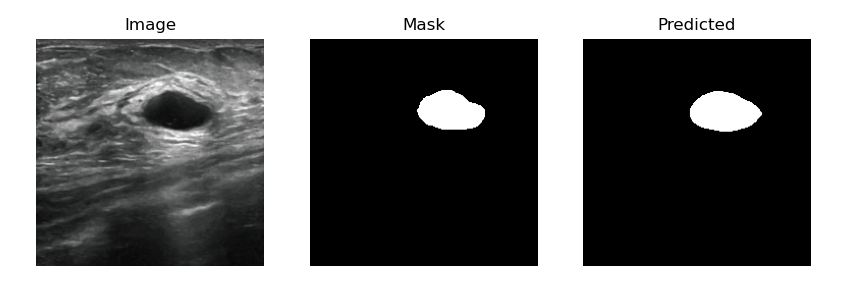
\includegraphics[width=\linewidth]{images/results/BUSI-unet7.png}
        \subcaption{}
        \label{fig:busi-unet1}
    \end{subfigure}    
    \vspace{1em}      
    \begin{subfigure}{1\textwidth}
        \centering
        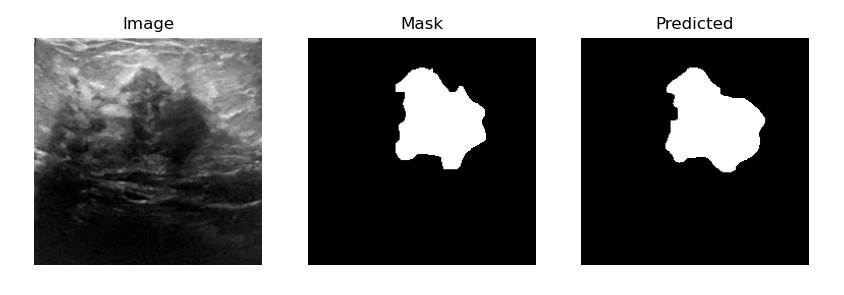
\includegraphics[width=\linewidth]{images/results/BUSI-unet6.png}
        \subcaption{}
        \label{fig:busi-unet2}
    \end{subfigure}
    \vspace{1em}
        \begin{subfigure}{1\textwidth}
        \centering
        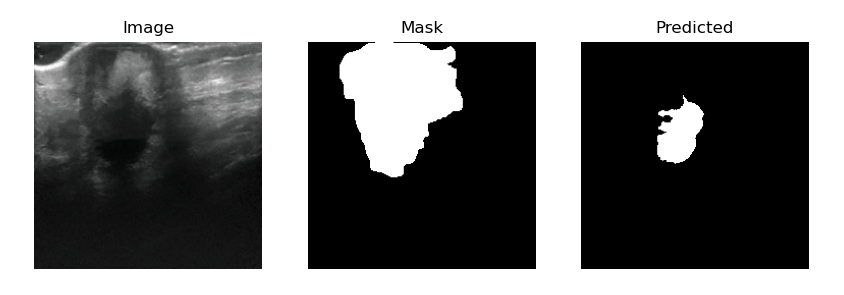
\includegraphics[width=\linewidth]{images/results/BUSI-unet1.png}
        \subcaption{}
        \label{fig:busi-unet3}
    \end{subfigure}
    \caption{Breast Tumor Segmentation results with UNet}
    \label{fig:busi-unet}
\end{figure}

\begin{figure}[]
    \centering
    \begin{subfigure}{1\textwidth}
        \centering
        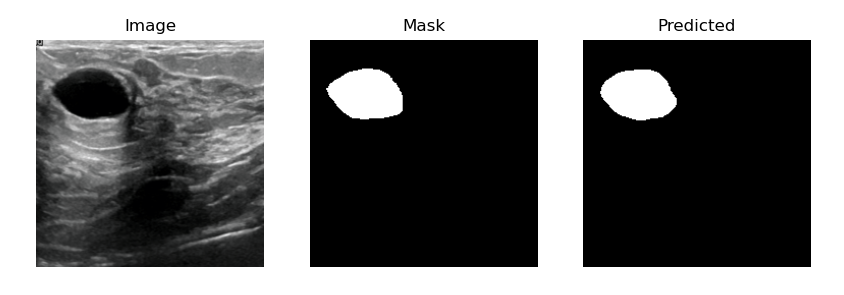
\includegraphics[width=\linewidth]{images/results/BUSI-maep.png}
        \subcaption{}
        \label{fig:busi-mae1}
    \end{subfigure}
    \vspace{1em}   
    \begin{subfigure}{1\textwidth}
        \centering
        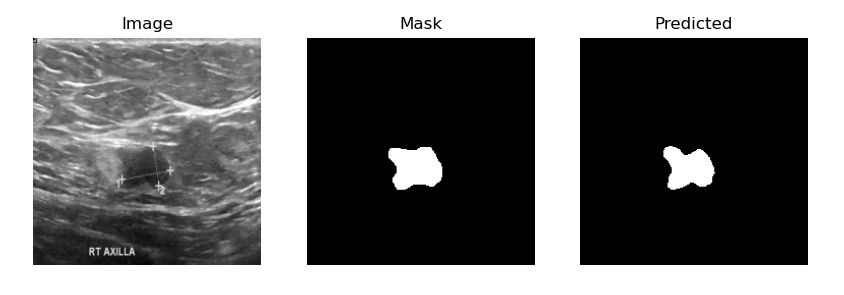
\includegraphics[width=\linewidth]{images/results/BUSI-mae7.png}
        \subcaption{}
        \label{fig:busi-mae2}
    \end{subfigure}
    \vspace{1em}
    \begin{subfigure}{1\textwidth}
        \centering
        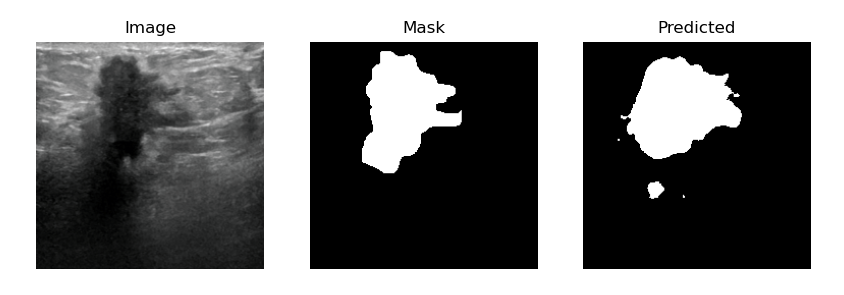
\includegraphics[width=\linewidth]{images/results/BUSI-mae11.png}
        \subcaption{}
        \label{fig:busi-mae3}
    \end{subfigure}
    \caption{Breast Tumor Segmentation results with MAE+UNETR}
    \label{fig:busi-mae}
\end{figure}

% BTS
\begin{figure}[]
    \centering
    \begin{subfigure}{1\textwidth}
        \centering
        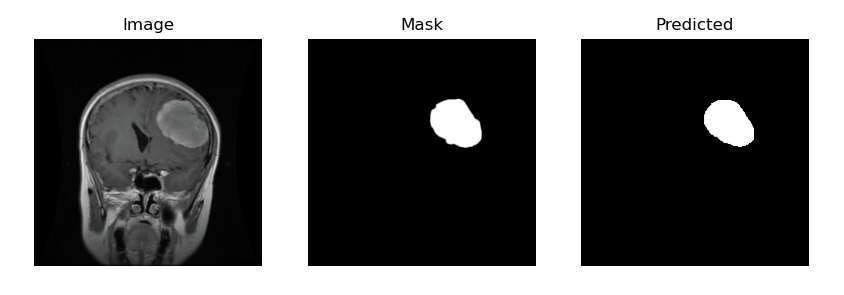
\includegraphics[width=\linewidth]{images/results/BTS-unet2.png}
        \subcaption{}
        \label{fig:bts-unet1}
    \end{subfigure}
    \vspace{1em}   
    \begin{subfigure}{1\textwidth}
        \centering
        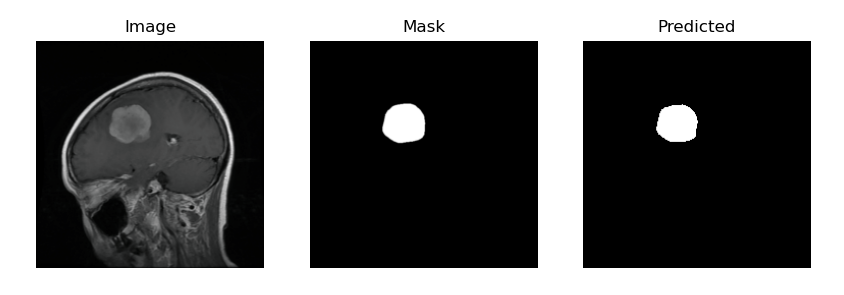
\includegraphics[width=\linewidth]{images/results/BTS-unet1.png}
        \subcaption{}
        \label{fig:bts-unet2}
    \end{subfigure}
    \vspace{1em}   
    \begin{subfigure}{1\textwidth}
        \centering
        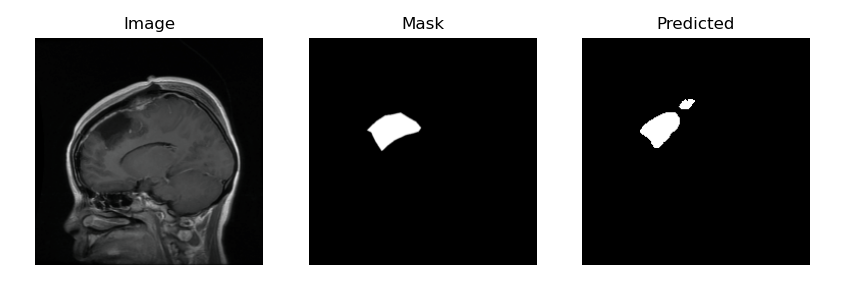
\includegraphics[width=\linewidth]{images/results/BTS-unet6.png}
        \subcaption{}
        \label{fig:bts-unet3}
    \end{subfigure}
    \caption{Brain Tumor Segmentation results with UNET}
    \label{fig:bts-unet}
\end{figure}

\begin{figure}[]
    \centering
    \begin{subfigure}{1\textwidth}
        \centering
        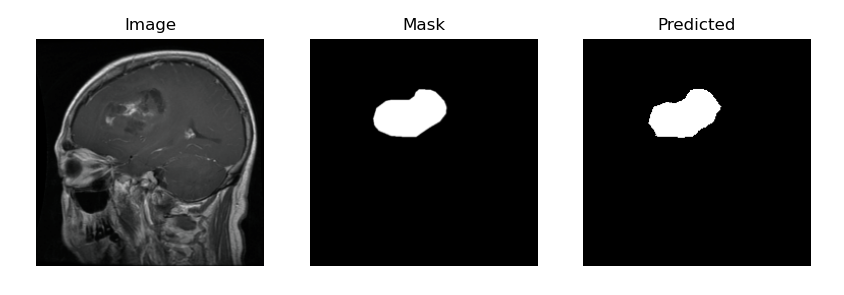
\includegraphics[width=\linewidth]{images/results/BTS-mae6.png}
        \subcaption{}
        \label{fig:bts-mae1}
    \end{subfigure}
    \vspace{1em}   
    \begin{subfigure}{1\textwidth}
        \centering
        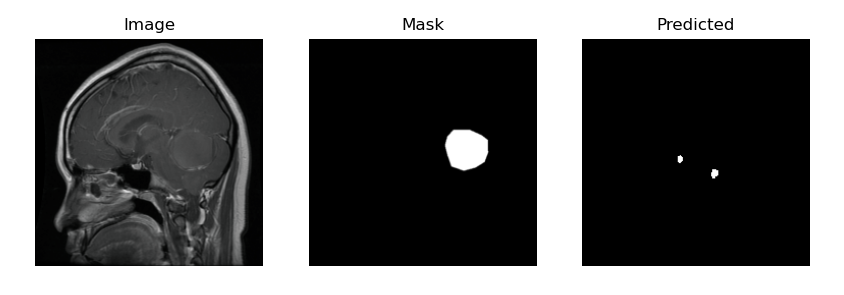
\includegraphics[width=\linewidth]{images/results/BTS-maecannato.png}
        \subcaption{}
        \label{fig:bts-mae2}
    \end{subfigure}
    \vspace{1em}   
    \begin{subfigure}{1\textwidth}
        \centering
        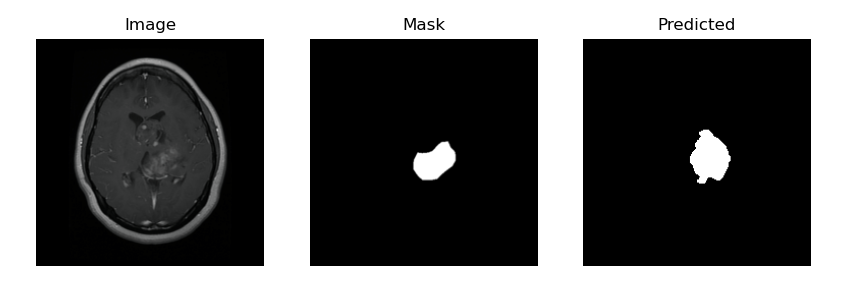
\includegraphics[width=\linewidth]{images/results/BTS-mae3.png}
        \subcaption{}
        \label{fig:bts-mae3}
    \end{subfigure}
    \caption{Brain Tumor Segmentation results with MAE+UNETR}
    \label{fig:bts-mae}
\end{figure}

% CVC
\begin{figure}[]
    \centering
    \begin{subfigure}{1\textwidth}
        \centering
        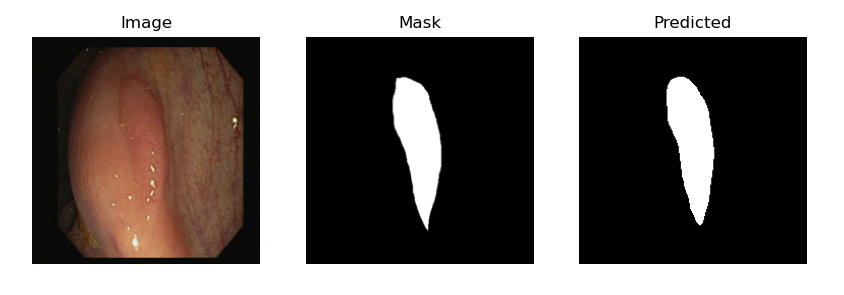
\includegraphics[width=\linewidth]{images/results/CVC-unet.png}
        \subcaption{}
        \label{fig:cvc-unet1}
    \end{subfigure}
    \vspace{1em}   
    \begin{subfigure}{1\textwidth}
        \centering
        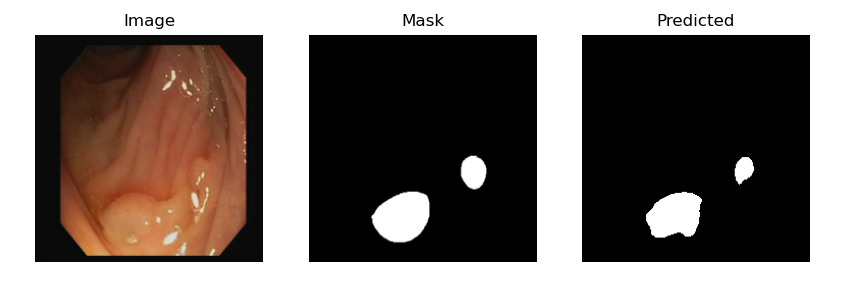
\includegraphics[width=\linewidth]{images/results/CVC-unet5.png}
        \subcaption{}
        \label{fig:cvc-unet2}
    \end{subfigure}
    \vspace{1em}   
    \begin{subfigure}{1\textwidth}
        \centering
        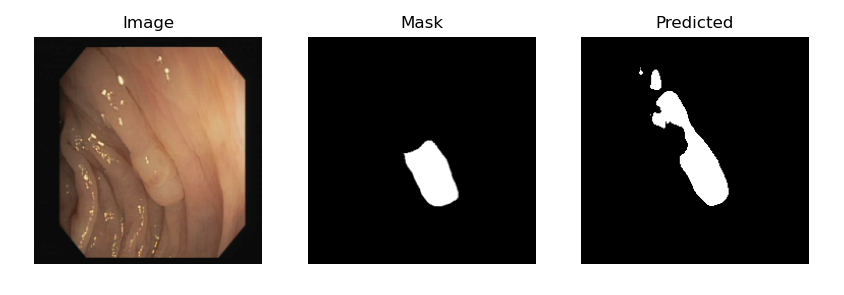
\includegraphics[width=\linewidth]{images/results/CVC-unet2.png}
        \subcaption{}
        \label{fig:cvc-unet3}
    \end{subfigure}
    \caption{Colon Polyp Segmentation results with UNET}
    \label{fig:cvc-unet}
\end{figure}

\begin{figure}[]
    \centering
    \begin{subfigure}{1\textwidth}
        \centering
        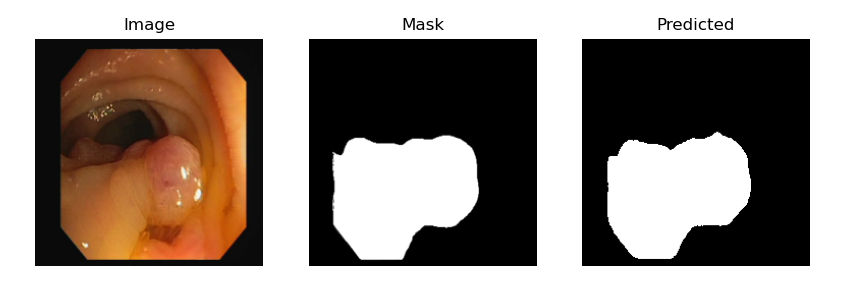
\includegraphics[width=\linewidth]{images/results/CVC-mae2.png}
        \subcaption{}
        \label{fig:cvc-mae1}
    \end{subfigure}
    \vspace{1em}      
    \begin{subfigure}{1\textwidth}
        \centering
        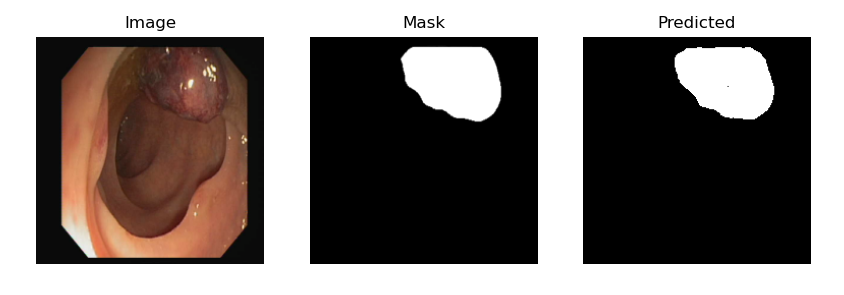
\includegraphics[width=\linewidth]{images/results/CVC-maep.png}
        \subcaption{}
        \label{fig:cvc-mae2}
    \end{subfigure}
    \vspace{1em}      
    \begin{subfigure}{1\textwidth}
        \centering
        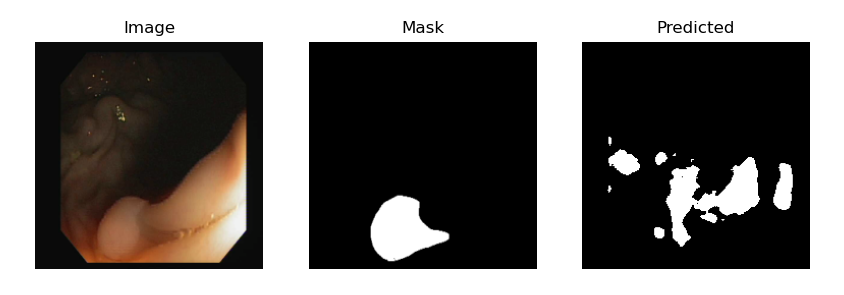
\includegraphics[width=\linewidth]{images/results/CVC-mae4.png}
        \subcaption{}
        \label{fig:cvc-mae3}
    \end{subfigure}
    \caption{Colon Polyp Segmentation with MAE+UNETR}
    \label{fig:cvc-mae}
\end{figure}
% \end{comment}

\newpage
%\addcontentsline{toc}{section}{Bibliography}
%\section*{Bibliography}
\printbibliography[heading=bibintoc,title={Bibliography}]


\end{document}